\RequirePackage{etoolbox}
\csdef{input@path}{%
 {sty/}% cls, sty files
 {img/}% eps files
}%
\csgdef{bibdir}{bib/}% bst, bib files

\documentclass[ba]{imsart}
%
\pubyear{0000}
\volume{00}
\issue{0}
\doi{0000}
\firstpage{1}
\lastpage{1}

%
\usepackage{amsthm}
\usepackage{amsmath}
\usepackage{natbib}
\usepackage[colorlinks,citecolor=blue,urlcolor=blue,filecolor=blue,backref=page]{hyperref}
\usepackage{graphicx}

\startlocaldefs

\endlocaldefs


%\usepackage{fullpage,amsmath}% mathtools}
%\usepackage{setspace}
\usepackage{graphicx, psfrag, amsfonts, float}
\usepackage{natbib}
\usepackage{amsthm}
\usepackage{multirow}
\usepackage{hhline}
%\usepackage{color}
%\usepackage[position=t,singlelinecheck=off]{subcaption}
%\usepackage{caption, setspace}
%\usepackage[position=t,singlelinecheck=off]{subfigure}
 \pdfminorversion=4
\usepackage{rotating}
\def\bgam{\mbox{\boldmath $\gamma$}}
\def\bth{\mbox{\boldmath $\theta$}}
\def\bbeta{\mbox{\boldmath $\beta$}}
\def\blam{\mbox{\boldmath $\lambda$}}
\def\bmu{\mbox{\boldmath $\mu$}}

\newcommand{\bx}{\mbox{\boldmath $x$}}
\newcommand{\bu}{\mbox{\boldmath $u$}}
\newcommand{\bc}{\mbox{\boldmath $c$}}
\newcommand{\bs}{\mbox{\boldmath $s$}}
\newcommand{\by}{\mbox{\boldmath $y$}}
\newcommand{\bz}{\mbox{\boldmath $z$}}
\newcommand{\bv}{\mbox{\boldmath $v$}}
\newcommand{\bb}{\mbox{\boldmath $b$}}
\newcommand{\bzero}{\mbox{\boldmath $0$}}
\newcommand{\thstarj}{\mbox{$\theta^\star_j$}}
\newcommand{\bths}{\mbox{$\btheta^\star$}}
\newcommand{\pkg}[1]{{\fontseries{b}\selectfont #1}} 

\newcommand{\ud}{\mathrm{d}}
\newcommand{\uI}{\mathrm{I}}
\newcommand{\uP}{\mathrm{P}}
\newcommand{\up}{\mathrm{p}}
\newcommand{\mb}{\mathbf}
\newcommand{\mc}{\mathcal}


\newcommand{\Bern}{\mbox{Bern}}
\newcommand{\Nor}{\mbox{N}}
\newcommand{\Ga}{\mbox{Gamma}}
\newcommand{\Dir}{\mbox{Dir}}
\newcommand{\Ber}{\mbox{Ber}}
\newcommand{\Be}{\mbox{Be}}
\newcommand{\Unif}{\mbox{Unif}}
\newcommand{\Binom}{\mbox{Bin}}
\newcommand{\IG}{\mbox{IG}}

\newcommand{\Xs}{X^\star}
\newcommand{\Lc}{{\cal L}}


\usepackage[dvipsnames,usenames]{color}
\newcommand{\yy}{\color{magenta}\it}
\newcommand{\jj}{\color{Black}\rm}
\newcommand{\yjnote}[1]{\footnote{\color{Brown}\rm #1 \color{Black}}}
\newtheorem{theorem}{Theorem}[section]
\newtheorem{definition}[theorem]{\bf Definition}
\newtheorem{lemma}[theorem]{\bf Lemma}
\newtheorem{corollary}[theorem]{\bf Corollary}
\newtheorem{proposition}[theorem]{\bf Proposition}
\newtheorem{assumption}[theorem]{\bf Assumption}
\newtheorem{example}[theorem]{\bf Example}
\newtheorem{remark}[theorem]{\bf Remark}


\newcommand{\iid}{\stackrel{iid}{\sim}}
\newcommand{\indep}{\stackrel{indep}{\sim}}

\doublespacing
\setlength{\textwidth}{6 in}

% commands for for editing
\usepackage{color}
\usepackage{ulem} % \sout
\newcommand{\red}[1]{{\color{red}#1}}
\newcommand{\blue}[1]{{\color{blue}#1}}
\newcommand{\brown}[1]{{\color{brown}#1}}
\newcommand{\green}[1]{{\color{green}#1}}
\newcommand{\magenta}[1]{{\color{magenta}#1}}
\DeclareMathOperator*{\argmin}{\arg\!\min}
\graphicspath{{figures/}{figs/}}


\makeatletter
\newcommand{\labitem}[2]{%
\def\@itemlabel{\textbf{#1}{.}}
\item
\def\@currentlabel{#1}\label{#2}}
\makeatother


%  Points to handle in preparing the manuscript
%
%  1.  Out of sample evaluation of the model.  We should go with trimmed mean log-likelihood (trimming the cases
%       that contribute least to log-likelihood).  Justification for the trimming mentioned in a sentence
%       here, to be more carefully and completely done in separate work (with Yoonsuh).  
%
%  3.  Add quite a number of references to Section 2.  This is where we should catch the old work
%      that conditions on the sample mean and proceeds through asymptotic approximation, Peter 
%      Hoff's work on ranks, Holmes and Walker's work, and ABC.  New text needs to accompany the
%      references, making clear what the other work does and how ours differs.  The new text should
%      be quite brief.  
%
%  4.  A big question.  Should we try to add any asymptotic theory?  A Section 3.4?  See next comment.  
%      My vote is "no".  
%
%  5.  Page limitations.  A goal for the entire manuscript is 30 pages.  Current length is 34+, spilling
%      onto page 35.  But, additions will include the abstract (1/2 page or so), conclusions (1 page or 
%      so), more references (another half page?), and more writing scattered throughout.  Redoing
%      figures (two to drop) and tables will save a modest amount of space.   I propose that we 
%      hold off on adding new content until we see how long the paper is.  Also, new content along
%      the lines of point 4 would mean that we have to prove/use existing results to show the truth
%      of whatever we claim!  
%
%  6.  Confirm with Nationwide that they are okay with our using their data and that they are comfortable
%       with the descriptions we have in the paper.  
%
%  7.  Fit the hierarchical model, conditioning on the robust summaries at each leaf in the model.  
%
%  9.  A hedge on computations?  There are examples (pathological in some senses) for which a basic
%      MCMC based on the complete data works, but where conditioning on a poorly chosen T(y) leads
%      to a reducible Markov chain.  I don't think this happens when the support of y is the same for all
%      \theta (it may be that mutual absolute continuity of all distributions for y|\theta is needed, though
%      definitions of "support" vary somewhat).  I think we can ignore this here, but an example could go
%      into the dissertation.  (one sentence now included to hint at this).  



%  To be added
%
%  1.  Abstract.  
%
%  2.  Conclusions.  To be written later.  I will take a pass at them once a few results are filled in for
%       the data analysis.  
%

%  John.  
%  See notes in red throughout.  The overarching goal is to move the manuscript toward completion.  
%  To do so means filling in details to get them taken care of.  Big batches are (i) references, (ii) 
%  deciding on notation for the estimator (b to replace beta?), (iii) verifying that the theorems have the
%  right conditions, (iv) patching figures, (v) adding material for the examples, and (vi) deciding whether
%  the figure and text on the last two pages is needed.  
%  If you want to add comments for us, pick a color other than red and add them in that color.  

%  Yoon.  
%  A check on the theorems would be great.  No need, I think, to dig out the paper by Miao and Ben Israel
%  as that part of the math is fine (I'll check to make sure that all conditions for our use of the theorems have
%  been stated in the Corollary).  Once more details are in place, proof reading and adjustment.  

%\newpage

\begin{document}

\begin{frontmatter}
\title{Bayesian Restricted Likelihood Methods: Conditioning on Insufficient Statistics in Bayesian Regression\thanksref{T1}}
\runtitle{Bayesian Restricted Likelihood Methods}
\thankstext{T1}{This research has been supported by Nationwide Insurance Company and by the NSF under grant numbers DMS-1007682 and DMS-1209194.  The views in this paper are not necessarily those of Nationwide Insurance or the NSF.} 

\begin{aug}
\author{\fnms{John R.} \snm{Lewis}\thanksref{addr1,m1}\ead[label=e1]{lewis.865@osu.edu}}, 
\author{\fnms{Steven N.} \snm{MacEachern}\thanksref{addr1,m1}\ead[label=e2]{snm@stat.osu.edu}}, 
\and  
\author{\fnms{Yoonkyung} \snm{Lee}\thanksref{addr1,m1}\ead[label=e3]{yklee@stat.osu.edu}} \\
%{\small \it Department of Statistics, The Ohio State University, Columbus, Ohio 43210}\\
%{\small lewis.865@osu.edu, snm@stat.osu.edu and yklee@stat.osu.edu}
\runauthor{J. Lewis et al}

\address[addr1]{Department of Statistics, The Ohio State University, Columbus, Ohio 43210 
    \printead{e1}, % print email address of "e1"
    \printead*{e2},
    \printead*{e3}
}
\end{aug}


\begin{abstract}
Bayesian methods have proven themselves to be successful across a wide
range of scientific problems and have many well-documented advantages
over competing methods. However, these methods run into difficulties
for two major and prevalent classes of problems: handling data sets
with outliers and dealing with model misspecification. We outline the
drawbacks of previous solutions to both of these problems (e.g., use of
heavy-tailed likelihoods) and propose a new method as an
alternative.  When working with the new method, we summarize
the data through a set of insufficient statistics,
targeting inferential quantities of interest, and update the prior
distribution with the summary statistics rather than the complete
data.  By careful choice of conditioning statistics, we
retain the main benefits of Bayesian methods while reducing the
sensitivity of the analysis to features of the data not captured by
the conditioning statistics. For reducing sensitivity to outliers,
classical robust estimators (e.g., M-estimators) are natural choices
for conditioning statistics. With these choices, the method can be thought of as a
blend of classical robust estimation and Bayesian methods. A major contribution of this work is the development of a data 
augmented Markov chain Monte Carlo (MCMC) algorithm
for the linear model and a wide range of choices for
summary statistics. We demonstrate the method on an
insurance agency data set containing many outliers and subject to model
misspecification. Success is manifested in better predictive
performance for data points of interest as compared to competing
methods.
\end{abstract}
%\noindent KEYWORDS: Approximate Bayesian computation, Markov chain
%Monte Carlo, M-estimation, Robust regression.

%\begin{keyword}[class=MSC]
%\kwd[Primary ]{60K35}
%\kwd{60K35}
%\kwd[; secondary ]{60K35}
%\end{keyword}

\begin{keyword}
\kwd{Approximate Bayesian computation}
\kwd{Markov chain Monte Carlo}
\kwd{M-estimation}
\kwd{Robust regression}
\end{keyword}

\end{frontmatter}

\section{Introduction}
Bayesian methods have provided successful solutions to a wide range of scientific problems, with their value
having been demonstrated both empirically and theoretically.  
In simple settings, the success of the methods is often attributed to formal optimality properties, sometimes derived
through the laws of subjective probability 
and sometimes through admissibility and the complete class
theorems of decision theory.  In complex settings, the hierarchical model allows one to create 
and fit sophisticated models that may, for example, pool information across similar problems.  

The development of Bayesian inference relies on a complete Bayesian model consisting of 
three elements:  the prior distribution, the loss function, and the likelihood or sampling density.  While formal optimality of Bayesian methods is unquestioned if one accepts the validity of all three of these elements, a healthy skepticism encourages us to question each of them.  Concern about the prior distribution has been addressed through the development of techniques for subjective elicitation \citep{garthwaite2005, ohagan2006} and objective Bayesian methods \citep{berger2006}.  
Concern about the loss function is reflected in, for example, the
extensive literature on Bayesian hypothesis tests \citep{kass1995}.  
%This work focus on the likelihood.  % sampling density has been given less attention from a specificallyBayesian view, although the work on predictive diagnostics \citep{box1980} departs from classical traditions.  

The focus of this work is the development of techniques to handle imperfections in the likelihood.  These imperfections often show themselves through the presence of outliers--cases 
not reflecting the phenomenon under study. There are three main solutions to Bayesian outlier-handling.  The first is to replace the basic sampling
density with a mixture model which includes one component for the ``good'' data and a second 
component for the ``bad'' data.  With this approach, the prior distribution is updated with the  mixture model likelihood to obtain the complete-data posterior distribution and  the good component of the sampling density is used for prediction of future good data.  The second approach replaces the
basic sampling density with a thick-tailed density in an attempt to discount outliers, yielding techniques that 
often provide solid estimates of the center of the distribution but 
do not easily translate to predictive densities for further good data.  The third approach fits a flexible (typically nonparametric) model to  the data, producing a Bayesian version of a density estimate for both good and bad data.  In recent development, inference 
is made through the use of robust inference functions \citep{lee2014}.  

The traditional strategies for handling outliers all have their drawbacks.  While we view the sampling density for the good data as stable, the outlier-generating processes 
may be transitory in nature, constantly shifting as the source of bad data changes.  This prevents us from appealing to large-sample arguments to claim that, with enough data, we can nail down a model for both good and bad data combined.  Instead of attempting to model both good and bad data, we propose a novel strategy for handling outliers. In a nutshell, we begin with a complete model  as if all of the data are good. Rather than driving the move from prior to posterior  by the full likelihood, we use only the likelihood
driven by a few summary statistics which typically target inferential quantities
of interest.  We call this likelihood a restricted because conditioning is done on a restricted set of data; the set which satisfies the observed summary statistics. This is a formal update of the prior distribution based on the sampling density of the summary statistics. The novelty of the work is twofold.  We make use of classical robust estimators as  summary statistics in a formal
Bayesian framework, using the sampling density of the estimators as a replacement for the 
sampling density of the data.  Second, we advance the argument that conditioning on an insufficient summary of the data is sound practice, rather than merely being done for computational and modelling convenience.  

% \red{[Steve, just a reminder that a paragraph about model misspecification was here orginally but commented out by John following a referee's suggestion. I also agree with the referee in that model misspecification could be a much broader issue than having a fraction of bad data while the model for good data is correctly specified.]}
%In addition to outlier-prone data, the 
%\green{ The sampling density can err due to other forms of model misspecification.  
%The traditional view is that, if the model is inadequate, one should build a better model.  In our
%empirical work, as data sets have become larger and more complex, we have bumped into 
%settings where we cannot realistically build the perfect model.  We ask the question ``by attempting
%to improve our model through elaboration, will the overall performance of the model suffer?''  If yes,
%we avoid the elaboration, retaining a model with some level of misspecification.  Acknowledging that
%the model is misspecified implies acknowledging that the sampling density is incorrect, as
%we do when outliers are present.  Thus, outliers are but one form of misspecified model.  
%We recommend a common solution for dealing with outliers and more general forms of model misspecification.}  

The remainder of the paper develops....  %Bayesian restricted likelihood (Section~\ref{restrictedlikelihood}), shows how it can be applied to a Bayesian linear model (Section~\ref{BayesLinMod}), illustrates its use on an insurance agencies data set with a novel twist on model evaluation (Section~\ref{Applications}), and wraps up with a discussion (Section~\ref{Conclusions}).  A major contribution of this work is the computational strategy whose legitimacy is established in Section~\ref{BayesLinMod}.  The technical proofs are in the appendix.   

\section{Restricted Likelihood}
\label{restrictedlikelihood}
%\textcolor{blue}{Tried to make more concise. Commented out section describing the further examples related to randomized experiments, contingency tables, and meta-analysis. }

\subsection{Examples}
To describe the use of the restricted likelihood, 
we begin with a pair of simple examples for the one-sample problem.  For both, the model takes the data $\by=(y_1,\ldots,y_n)$ to be a random sample
of size $n$ from a continuous distribution indexed by a parameter
vector $\bth$, with pdf $f(y| \bth)$.  The standard, or full,
likelihood is $L(\bth | \by) = \prod_{i=1}^n f(y_i | \bth)$.  

The first example considers the case where a known subset of the data are known to be 
bad in the sense of not informing us about $\bth$.  This case mimics the setting where outliers are identified and discarded before doing a formal analysis.  Without loss of generality, we label the good cases $1$ through $n-k$ and the bad cases $n-k+1$ through $n$.  The relevant likelihood to be used to move from prior distribution to posterior distribution is clearly $L(\bth | y_1, \ldots, y_{n-k}) = \prod_{i=1}^{n-k} f(y_i | \bth)$.  For an equivalent analysis, we rewrite the full likelihood as the product of two pieces:
\begin{eqnarray}
\label{OutlyingCases}
L(\bth | \by)  
= \left( \prod_{i=1}^{n-k} f(y_i | \bth) \right) \left( \prod_{i=n-k+1}^{n} f(y_i | \bth) \right) .  
\end{eqnarray}
We wish to keep the first piece and drop the second for better inference on $\bth$.

The second example involves deliberate censoring of small and large observations. This is
sometimes done as a precursor to the analysis of reaction time experiments  \citep[e.g.,][]{ratcliff1993} where very small and large reaction times are physiologically implausible;  explained by either anticipation or lack of attention of the subject.  
With lower and upper censoring times at $t_1$ and $t_2$, the post-censoring sampling distribution is of mixed form, with masses $F(t_1|\bth)$ at $t_1$ and $1-F(t_2|\bth)$ at $t_2$,
and density $f(y | \bth)$ for $y \in (t_1, t_2)$.  We adjust the original data $y_i$,
producing $c(y_i)$ by defining $c(y_i)= t_1$ if $y_i \leq t_1$, $c(y_i)=t_2$ 
if $y_i \geq t_2$, and $c(y_i)=y_i$ otherwise.  
The adjusted update is performed with $L(\bth |c(\by))$.  
Letting $g(t_1|\bth) = F(t_1|\bth)$,
$g(t_2 | \bth) = 1 - F(t_2|\bth)$, and $g(y|\bth)=f(y|\bth)$ for
$y \in (t_1, t_2)$, we may rewrite the full 
likelihood as the product of two pieces
\begin{eqnarray}
\label{Censoring} 
L(\bth | \by) =  \left( \prod_{i=1}^n g(c(y_i)  | \bth) \right) \left( \prod_{i=1}^n f(y_i|\bth,c(y_i)). \right) ,  
\end{eqnarray}
Only the first part is retained the analysis. Several more examples are detailed in \cite{lewis2014}.



%Further examples abound. In a completely randomized experimental design, we randomize %our 
%experimental units to treatment conditions and then ignore the details of the observed randomization \citep{dean1999}; 
%in work with contingency tables,  
%we collapse categories with small counts, coarsening the scale of %our 
%data \citep{agresti2002}; in meta-analysis, we ignore the individual patient-level data and instead
%work with estimated effects from the studies \citep{orourke2007}.  
%Further examples are described in \cite{lewis2014}. 
\subsection{Generalization}

To generalize the approach in \eqref{OutlyingCases} and
\eqref{Censoring}, %, and these other settings,
we write the full likelihood in two pieces with a conditioning statistic $T(\by)$, as indicated below:
\begin{eqnarray}
\label{FullLikelihood}
L(\bth | \by)  
& = & f(T(\by) | \bth) \,\, f(\by |\bth, T(\by)) .  
\end{eqnarray}
%Throughout the paper, we use the convention that a function is defined by its inputs. 
Here,  $f(T(\by) | \bth)$ is the conditional pdf of $T(\by)$ given $\bth$ and $f(\by |\bth, T(\by))$ is the conditional pdf of $\by$ given $\bth$ and $T(\by)$.  In the dropped case example, the conditioning statistic is $T(\by) = (y_1, \ldots, y_{n-k})$.  In 
the censoring example, the conditioning statistic is $T(\by) = (c(y_1),\ldots,c(y_n))$.  We refer to 
$f(T(\by) | \bth)$ as the restricted likelihood and $L(\bth | \by)=f(\by|\bth)$ as the full likelihood.  

Bayesian methods can make use of a restricted likelihood %in place of a complete likelihood
since $T(\by)$ is a well-defined random variable with a probability distribution indexed by $\bth$.  
This leads to the restricted likelihood posterior 
\begin{eqnarray}
\label{RestrictedPosterior}
\pi(\bth | T(\by)) & = & \frac{\pi(\bth) f(T(\by) | \bth)}{m(T(\by))} ,
\end{eqnarray}
where $m(T(\by))$ is the marginal distribution of $T(\by)$ under the prior distribution.  
Predictive statements for further (good) data rely on the model.  For another observation,
say $y_{n+1}$, we would have the predictive density 
\begin{eqnarray}
\label{RestrictedpredDist}
f(y_{n+1} | T(\by)) = \int f(y_{n+1} | \bth) \pi(\bth | T(\by))\ d\bth .  
\end{eqnarray}

\subsection{Literature review}
Direct use of restricted likelihood appears in many areas of the literature.  The motivation is often similar to ours:   
concern about outliers or, more generally, model misspecification.  For example, the use of rank likelihoods is discussed by \cite{savage1969}, \cite{pettitt1983, pettitt1982}, and more recently by \cite{hoff2013}.  
\cite{lewis2012} make use order statistics and robust estimators for $T(\by)$ in the location-scale setting. 
Asymptotic properties of restricted posteriors are studied by \cite{doksum1990}, \cite{clarke1995}, \cite{yuan2004},  and \cite{hwang2005}. The tenor of these asymptotic 
results is that, for a variety of conditioning statistics with non-trivial regularity conditions on prior, model, and likelihood, the
posterior distribution resembles the asymptotic sampling distribution of the conditioning statistic.  

Restricted likelihoods have also been used as practical approximations to a full likelihood. For example, \cite{pratt1965} appeals to heuristic arguments regarding approximate sufficiency to justify the use of the restricted likelihood of the sample mean and standard deviation. Approximate sufficiency is also appealed to in the use of Approximate Bayesian Computation (ABC), which is related to our method.  
ABC is a collection of posterior approximation methods which has recently experienced success in applications to epidemiology, genetics, and quality control \citep[see, for example,][]{tavare1997, pritchard1999,  marjoram2003, fearnhead2012}. Interest typically lies in the full data posterior and ABC is used for computational convenience as an approximation.  Consequently, effort is made to choose an approximately sufficient $T(\by)$ and update to the ABC posterior by using the likelihood $L(\bth| \mathcal{B}(\by))$, where $\mathcal{B}(\by)=\{\by^{*}|\rho(T(\by),T(\by^{*}))<\epsilon\}$, $\rho$ is a metric, and $\epsilon$ is a tolerance level. This is the likelihood ``conditioned'' on the collection of data sets which result in a $T(\cdot)$ within $\epsilon$ of the observed $T(\by)$. %Hence, we can see that, as in our method, conditioning is done on a summary of the complete data. 
With an approximately sufficient $T(\cdot)$ and a small enough $\epsilon$, heuristically  $L(\bth|\mathcal{B}(\by))\approx L(\bth|T(\by))\approx L(\bth|\by)$. Consequently, the ABC posterior approximates the full data posterior and efforts have been made to formalize what is meant by  approximate sufficiency \citep[e.g.,][]{joyce2008}. ABC is related to our method in that the ``conditioning'' is on something other than the data $\by$.  However, we specifically seek to condition on an insufficient statistic to guard against misspecification in parts of the likelihood. Additionally, we develop methods where the conditioning is exact (i.e. $\epsilon = 0$).


%ABC is related to our method in that conditioning is on something other than the complete data. Even if $T(\by)$ were exactly  sufficient in the traditional sense, a positive $\epsilon$ would result in something theoretically different from the complete data posterior (even if they are indeed approximately the same). We also mention that in ABC, $\mathcal{B}(\by)$ is not a statistic in the strict sense because it does not partition the sample space before observing data. That is, a feasible data set $\bz^{*}$ can belong to more than one `ball'  $\mathcal{B}(\cdot)$.  The method relies on conditioning on this set because in most ABC applications, approximating the complete data posterior directly is hard (or impossible) and sampling data matching the observed summary exactly is also hard (or impossible). ABC methods are a practical and useful solution in these settings. For the regression models we present, sampling new data matching the observed summary exactly is indeed possible and so we can condition exactly on the observed summary. Further, we reiterate that our motivation is different from ABC in that we do not want to condition on the complete data because we assume it contains inherent flaws which can be detrimental to inference. 

%However, the conditioning in ABC is heuristic.  For technical reasons, the calculation proceeding from $\pi(\bth)$ to $\pi(\bth)L(\bth| \mathcal{B}(\by))/\int \pi(\bth)L(\bth| \mathcal{B}(\by)) d\bth$ is not a formal conditional update.  Simply put, if an external observer told $\mathcal{B}(\by)$ can supply $T(\by)$ and vice-versa, the information contained in $\mathcal{B}(\by)$ is exactly that contained in $T(\by)$ and proper conditioning will lead to identical posterior distributions.  This is not the case with a typical implementation of ABC.  

% In a related, but distinctly different, approach which also takes advantage of summary statistics, the full data log likelihood is replaced by a loss function \citep[e.g.][]{bissiri2013} in an effort to concentrate inference only on parameters of interest. In contrast, the incomplete likelihood is formulated using a full probability model, allowing for a formal Bayesian update, while remaining robust to misspecification.

This work extends the development of Bayesian restricted likelihood by arguing that deliberate choice of $T(\by)$ is sound practice and also by expanding the class of conditioning statistics in which exact conditioning can be achieved.  Our methods do not rely on asymptotic properties, nor do they rely on approximate conditioning.%, \green{nor do they need to correspond to artificial censoring to create incomplete or missing data}  \citep[e.g.,][]{albert1988, hoffwakefield2013}.  
%\green{Note - fix references here hoffwakefield for asymptotic; albert for ? .}  

%The key to productive use of the restricted likelihood is the choice of $T(\by)$ and the development
%of computational strategies that allow us to truly condition on the observed $T(\by)$ and 
%fit the model in formal Bayesian fashion.  In this work, we focus
%on robustness, and natural choices of $T(\by)$ for the one-sample problem include a set of middling order statistics, a trimmed
%mean, or a classical robust estimator of location and/or scale.  
%We have previously implemented several of these methods and have found them to perform well \citep[][]{lewis2012}. Versions most extensible to the linear model include the M-estimators in the tradition of \cite{huber1964}, least median squares (LMS), and least trimmed squares (LTS). For these choices the restricted likelihood is not available in closed form, making computation of the restricted posterior a challenge. For low-dimensional statistics $T(\by)$ and parameters $\bth$, the direct computational strategies described in \cite{lewis2014} can be used to estimate the incomplete posterior conditioned on essentially any statistic.  These strategies rely on generation of complete data sets from different values of $\bth$.  
%Each complete data set leads to a statistic $T(\by)$ under $\bth$, and these generated statistics are used to estimate the density at $T(\by_{obs})$, where $\by_{obs}$ is the observed complete data. This estimate is fed into Bayes' theorem for the update from prior distribution to posterior distribution.  


%For the example in the previous section, these strategies work well.
%\textcolor{blue}{Comment out `A variety of  variance reduction techniques which exploit\dots' because it seemed too vague and a bit off topic}
%In low dimensional settings (in $T(\by)$ and $\bth$) the incomplete posterior under each of these versions (and others) can be estimated by approximating the incomplete likelihood using kernel density estimation techniques \citep[for details see][]{lewis2014}. 

%These direct sampling techniques rely on density estimation and numerical integration. Density estimation becomes difficult for high dimensional $T(\by)$ and numerical integration breaks down for high dimensional $\bth$. For these settings, an MCMC algorithm is developed in Section \ref{highDim}. Software is available from the authors for use with simultaneous M-estimators of location and scale. At the present time, further software development is required to extend beyond simultaneous M-estimators.  

%\textcolor{blue}{Added a bit about this to the discussion: Though we concentrate in this paper on applying incomplete likelihood inference for the mean of linear regression models, the computational strategies we devise in subsequent sections also allow us to apply the method to inference beyond the mean.  In particular, quantile regression falls within the framework we develop. }
%The next section develops the necessary computational strategies.  

%\subsection{Details of Examples in Section \ref{illustrations}}
%\subsubsection{Speed of Light}
%With parameters $\beta$ and $\sigma$, the full model is $\beta\sim N(23.6, 2.04^{2})$, $\sigma^{2}\sim IG(5, 10)$, $y_{i}\iid N (\beta, \sigma^{2})$ for $i=1,2,\dots, n=66$ where $y_{i}$ denotes the $i^{th}$ measurement of the passage time of light. $\beta$ is interpreted as the passage time of light with
%$\sigma^{2}$ representing measurement error. Tuning parameters for the M-estimators are chosen to achieve $95\%$ efficiency under normality and for comparability, roughly $5\%$ of the residuals are trimmed for LTS.  The t-model assumes $y_{i}\iid t_{\nu} (\beta, \sigma^{2})$ with $\nu=5$. The prior on $\sigma^{2}$ is $IG(5, \frac{\nu-2}{\nu}10)$ so the prior on the variance is the same as the other models. %We note that the variance of the data under this model is $\frac{\nu}{\nu-2}\sigma^{2}$.  For comparability, it is this quantity that has the prior distribution $IG(a,b)$ given above.   \citep[for details see][]{huber2009}





\section{Illustrative Examples}
\label{illustrations}
Before discussing computational details, the method is applied to two simple examples on well known data sets to demonstrate its effectiveness in situations where outliers are a major concern. The full model in each case fits into the Bayesian linear regression framework discussed in Section \ref{BayesLinMod}. %Specific details are left to the Appendix. 

The first example is an analysis of Simon Necomb's 66 measurements of the speed of light; two of which are significant outliers in the lower tail. The full model is a standard location-scale Bayesian model:
\begin{equation}
\beta\sim N(23.6, 2.04^{2}),\  \sigma^{2}\sim IG(5, 10), \ y_{i}\iid N (\beta, \sigma^{2}), i=1,2,\dots, n=66,
\end{equation}
where $y_{i}$ denotes the $i^{th}$ measurement of the passage time of light. $\beta$ is interpreted as the passage time of light with $\sigma^{2}$ representing measurement error.
Four versions of the restricted likelihood are fit with conditioning statistics: 1) Huber's M-estimator for location with Huber's `proposal 2'  for scale 2)  Tukey's M-estimator for location with Huber's `proposal 2'  for scale 3) LMS (least median squares) for location with associated estimator of scale and 4) LTS (least trimmed squares)  for location with associated estimator of scale. Associated tuning parameters for the M-estimators are chosen to achieve $95\%$ efficiency under normality \citep{huber2009} and for comparability, roughly $5\%$ of the residuals are trimmed for LTS.  Additionally, two other common approaches to outlier handling are fit: 1) replacing the normal distribution with a t-distribution and, 2) replacing the normal distribution with a mixture of two normals. The t-model assumes $y_{i}\iid t_{\nu} (\beta, \sigma^{2})$ with $\nu=5$. The prior on $\sigma^{2}$ is $IG(5, \frac{\nu-2}{\nu}10)$ so the prior on the variance is the same as the other models. The mixture takes the form: $y_{i}\iid pN (\beta, \sigma^{2}) + (1-p)N(\beta, 10\sigma^{2})$ assuming the prior $p \sim \beta(20,1)$ on the probability of belonging to the `good' component.  

The posteriors of $\beta$ under each model appear in Figure \ref{fig:newcomb_post}. As expected, the posterior under the normal model is pulled downward by the two outliers while the heavy tailed model provides robustness against them. The restricted likelihood methods using the M-estimators and LTS statistics also achieve robustness against the outliers. Conditioning on LMS however, results in a posterior similar to the one under the normal model. The M-estimators provide the most precise posteriors in this case. This is reflected in more precise predictions than the heavy-tailed and mixture model as illustrated by the predictive distributions displayed in  Figure \ref{fig:newcomb_predictive}.
\begin{figure}[t]
\centering
{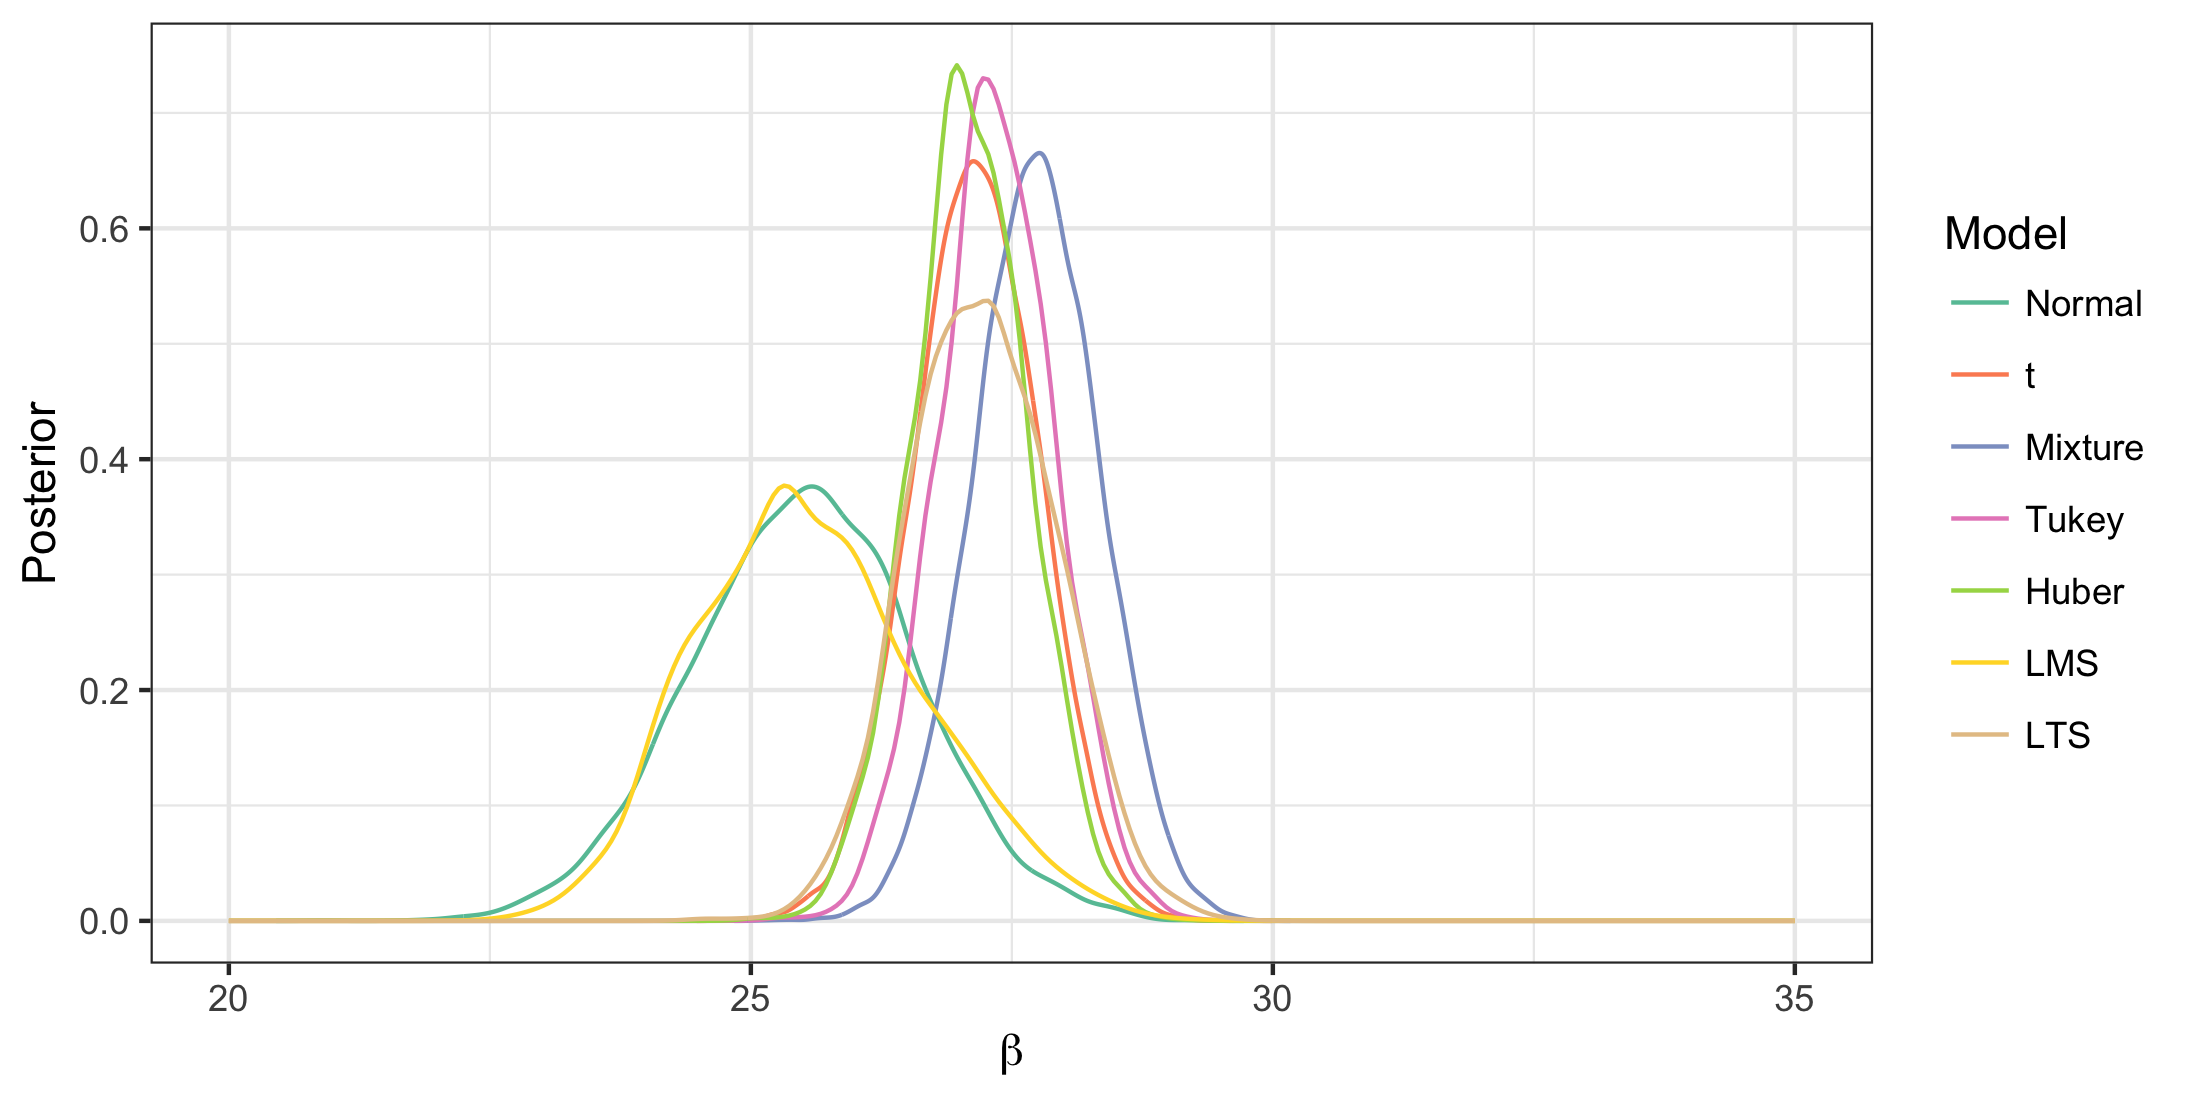
\includegraphics[width = 4in]{figs/speed_of_light_beta.png}}
{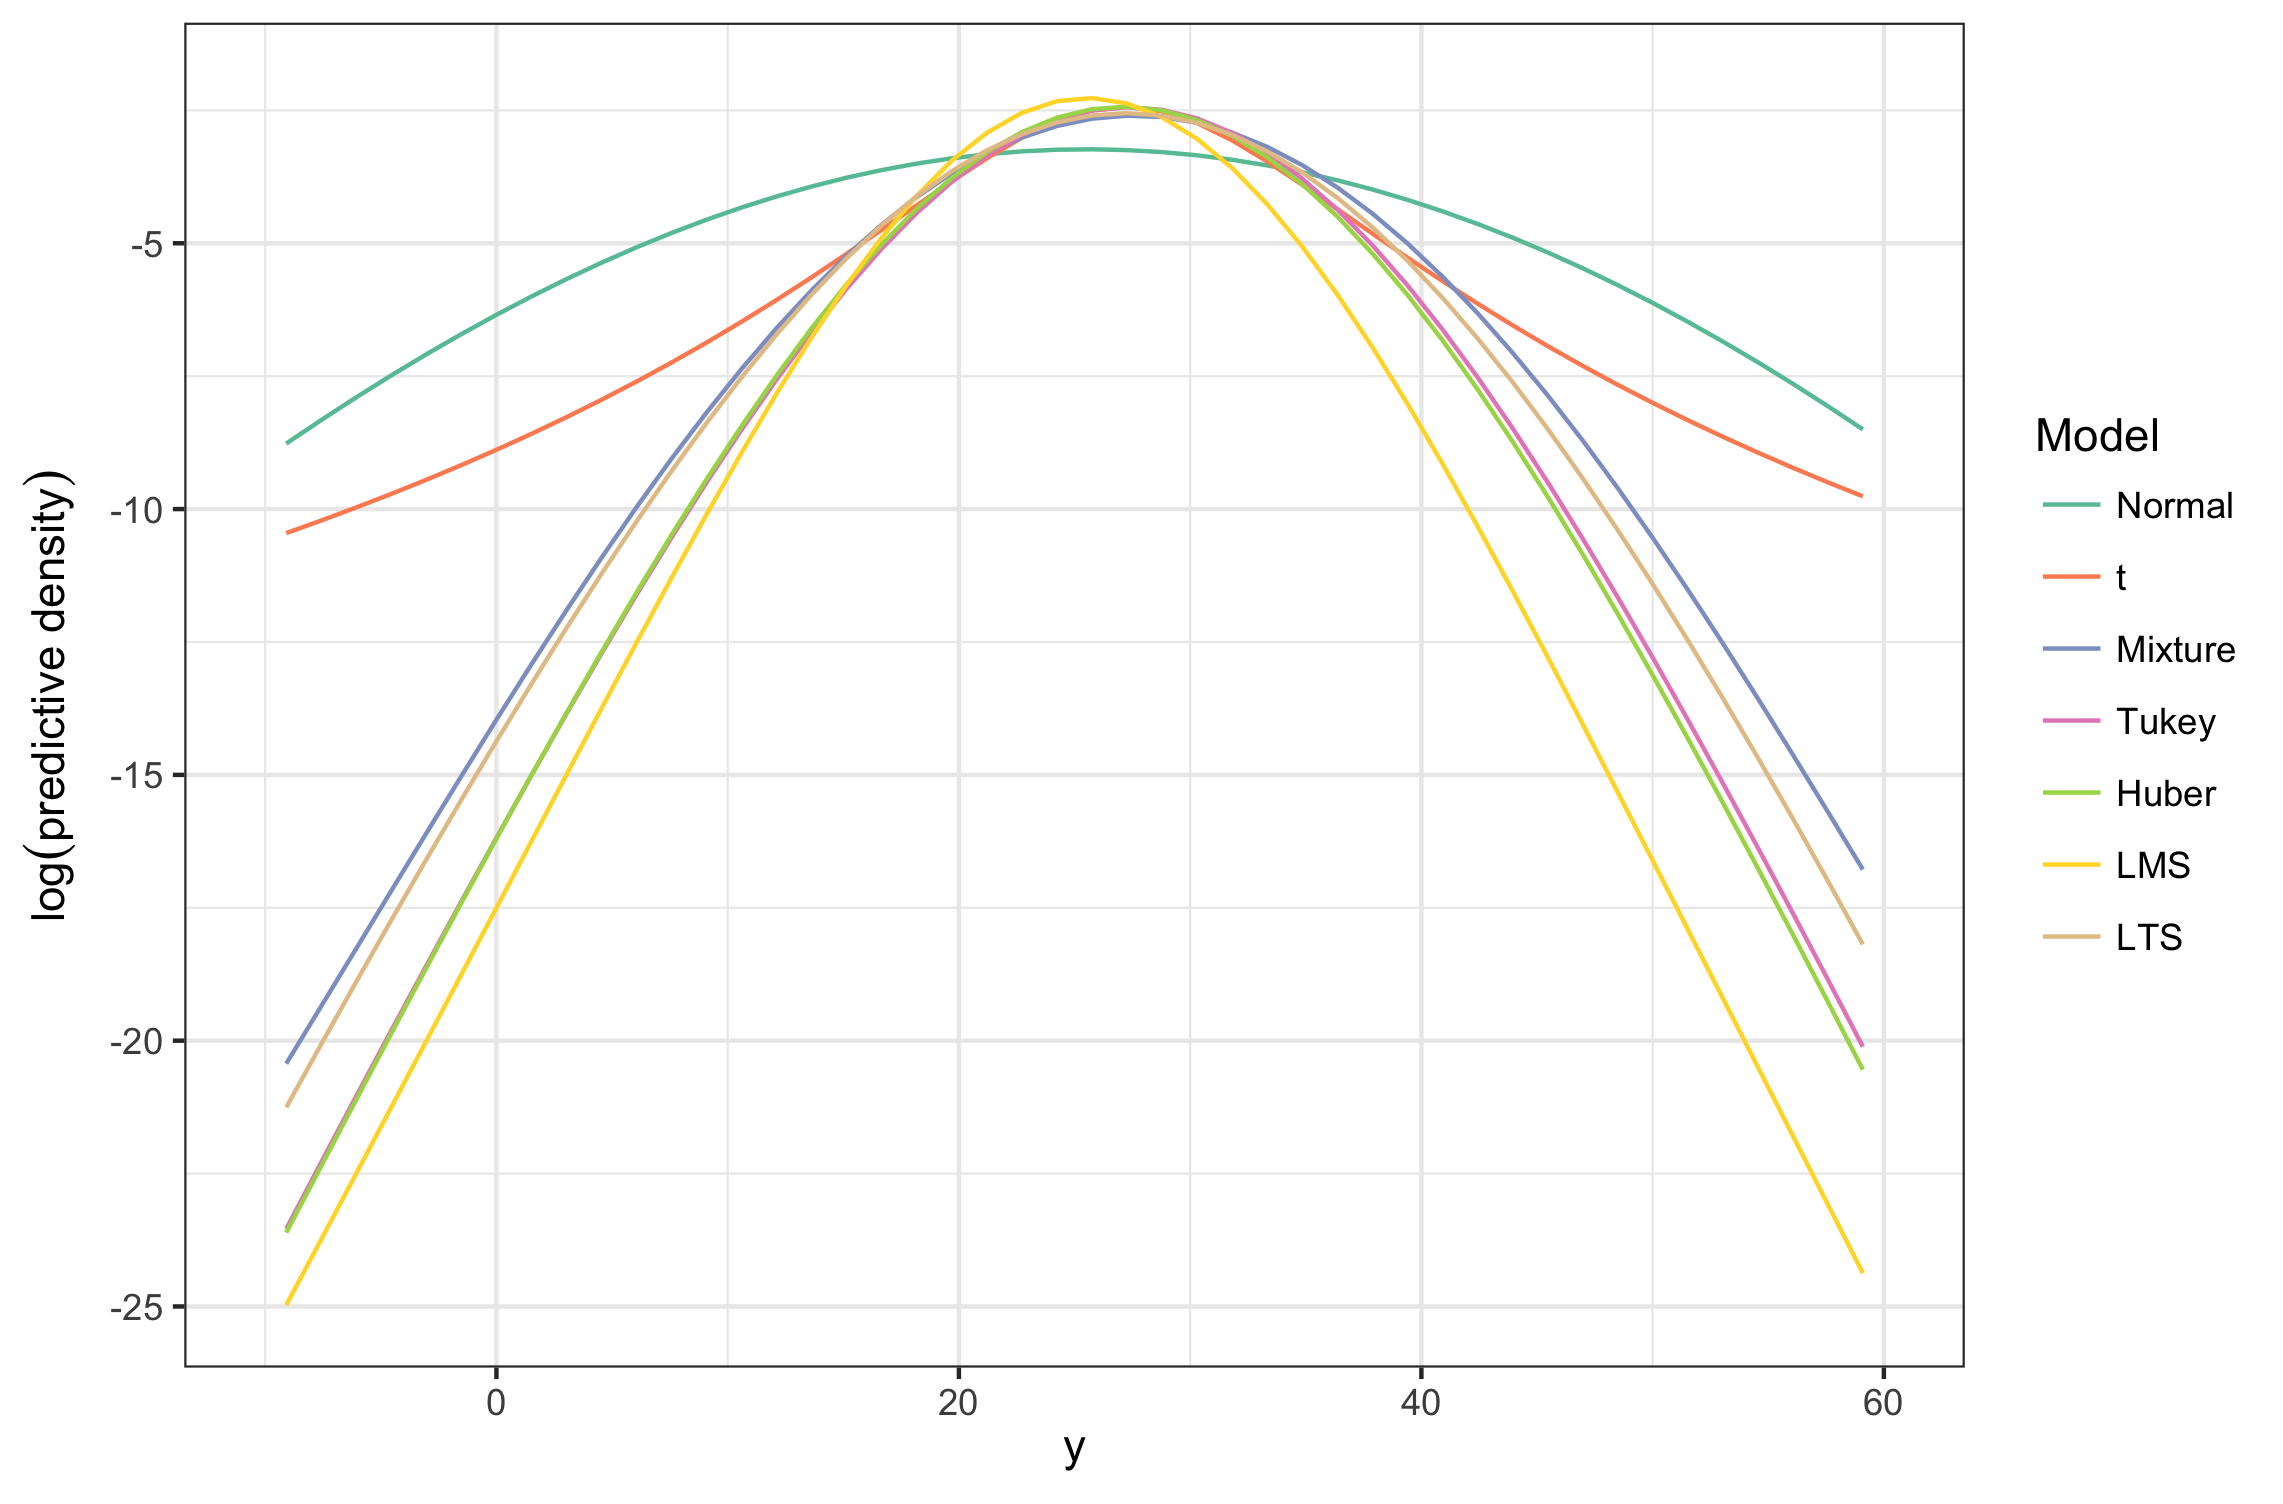
\includegraphics[width = 4in]{figs/speed_of_light_predictive.png}}
\caption{asdfdfa}
\label{fig:newcomb_post}
\end{figure}

%\begin{figure}[t]
%\centering
%{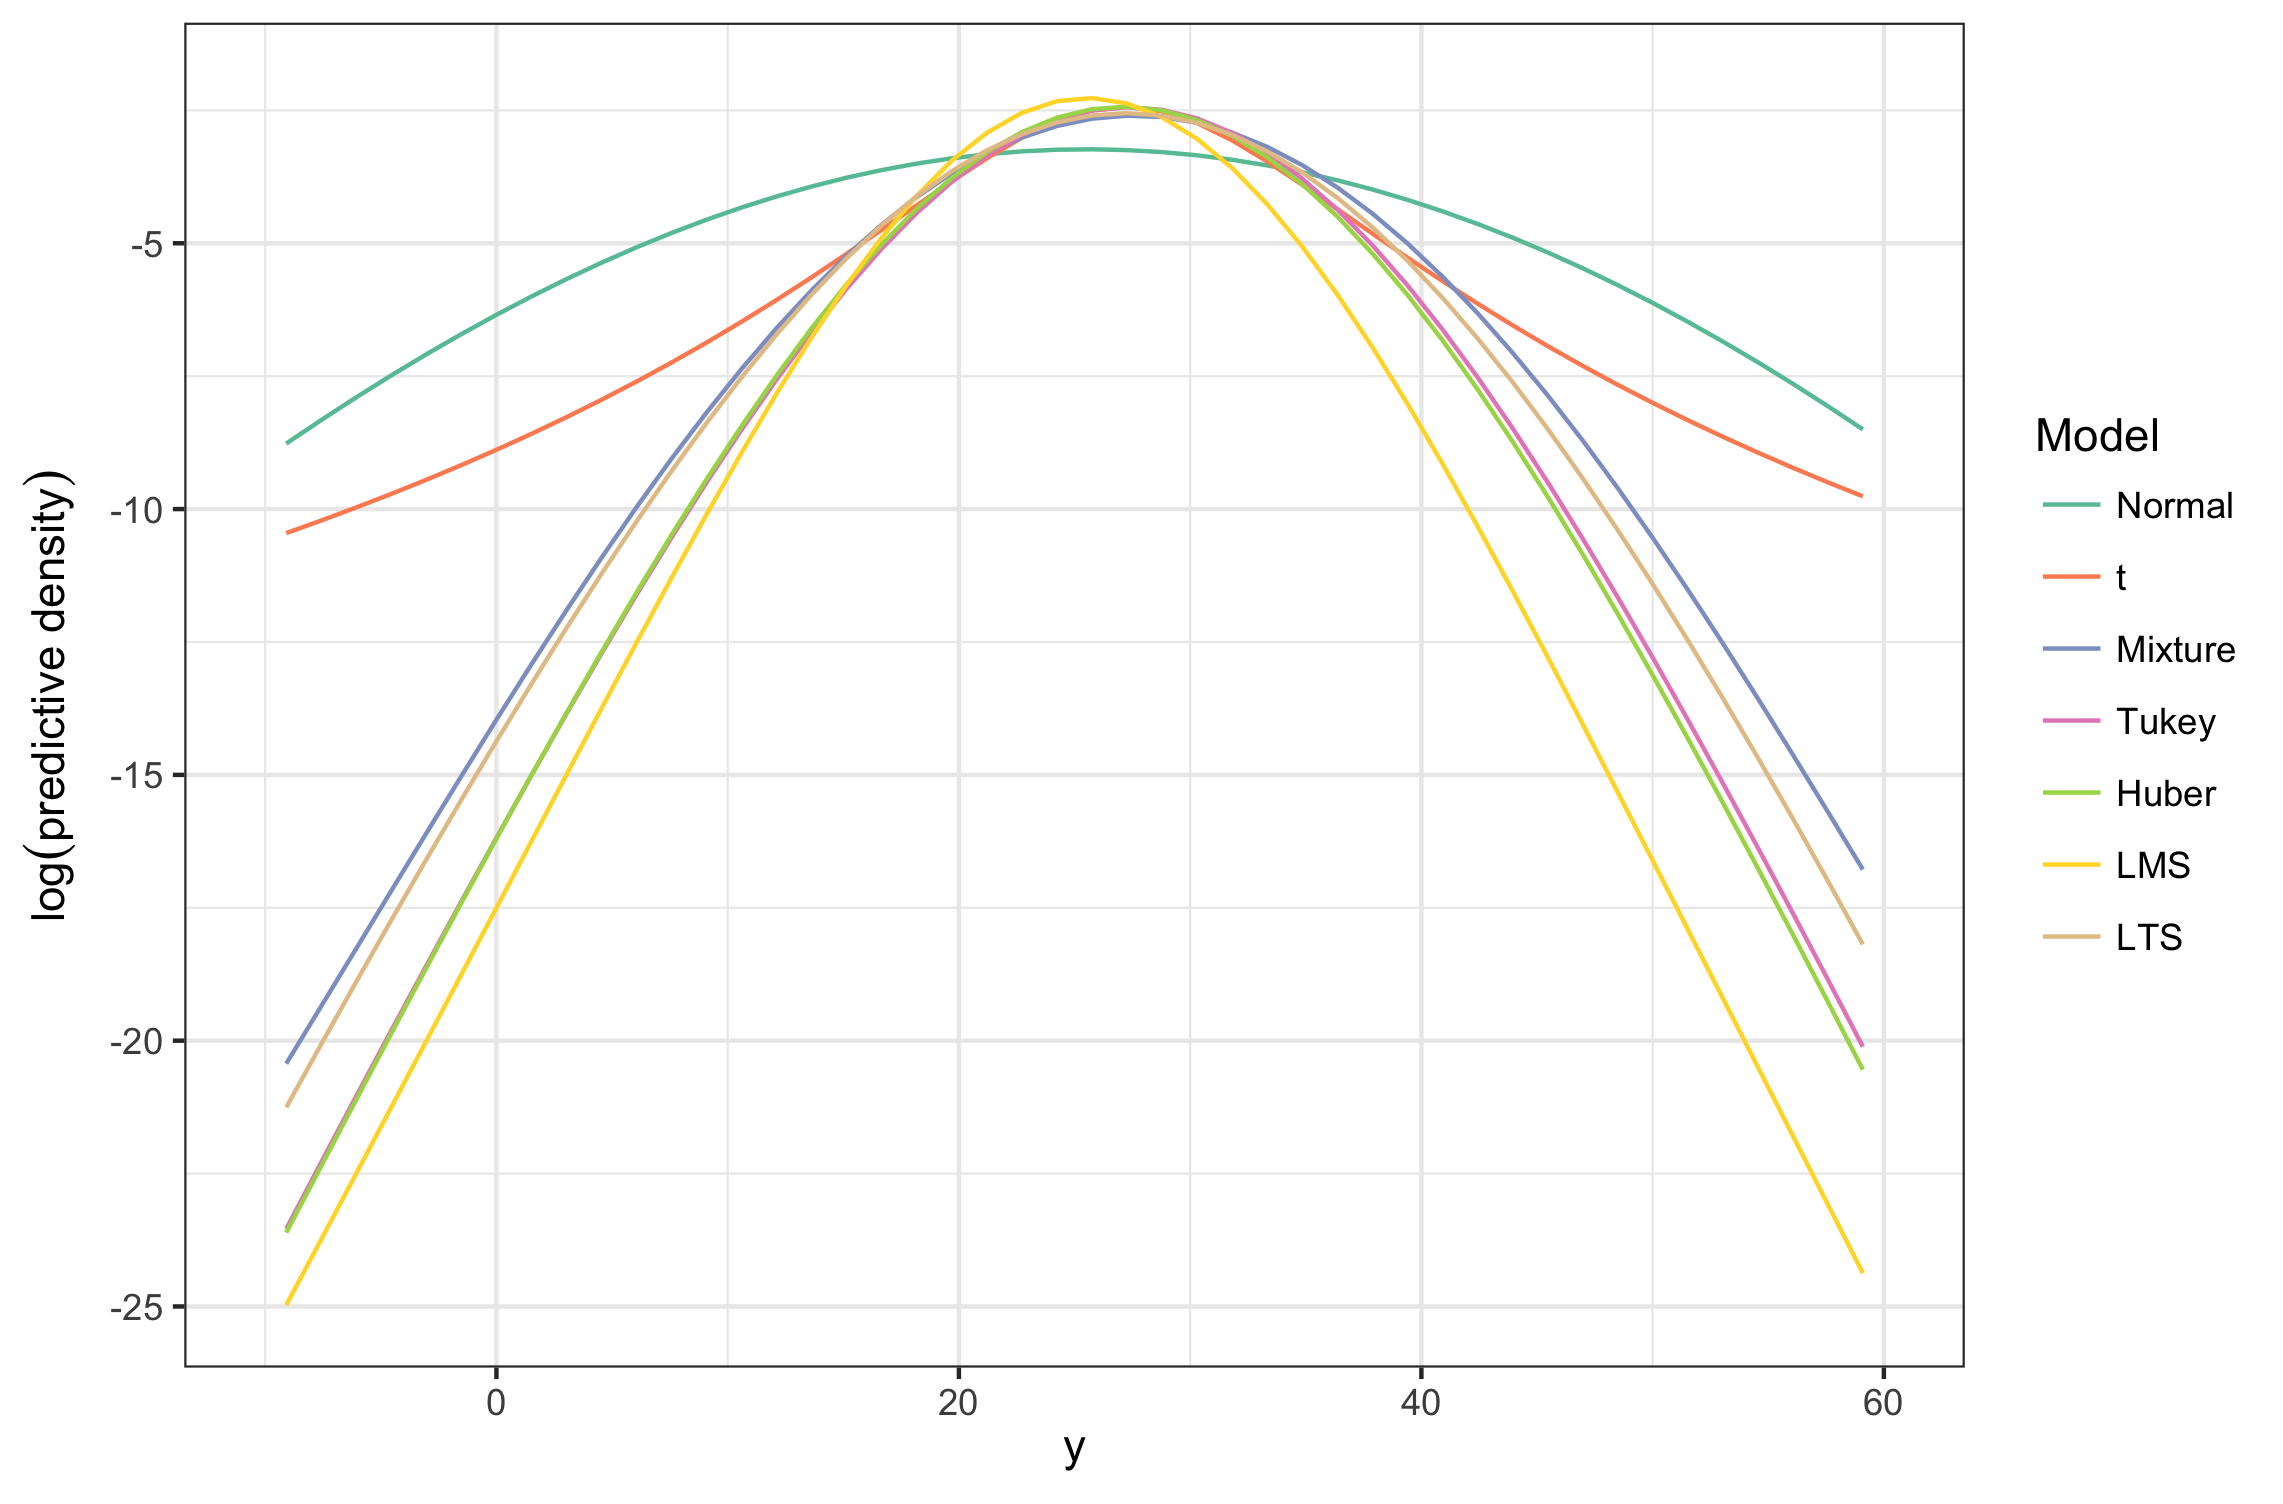
\includegraphics[width = 4in]{figs/speed_of_light_predictive.png}}
%\caption{dfsfsa}
%\label{fig:newcomb_predictive}
%\end{figure}
%\caption{Top: Posteriors of the location parameter $\beta$ under the normal theory model, the t-model, and four restricted likelihood models for Newcomb's speed of light measurements. Bottom: Posterior predictive distribution of the speed of light under the normal theory model, the t-model, and four restricted likelihood models.}
%\label{fig:newcomb_post}
%\end{figure}

As a second example, a data set measuring the number of telephone calls in Belgium from 1950-1973 is analyzed. The outliers in this case are due to a change in units on which calls were recorded for part of the dataset. The full model is a standard normal Bayesian linear regression:

\begin{equation}
{\boldsymbol{\beta}}\sim N_{2}(\boldsymbol{\mu}_{0}, \boldsymbol{\Sigma}_{0}),\  \sigma^{2} \sim IG(a, b), \by \sim N(X\boldsymbol{\beta}, \sigma^{2} I),
\end{equation}
where $\bbeta = (\beta_{0}, \beta_{1})^{\top}$, $\by$ is the vector of the logarithm of the number of calls, and X is the $n\times 2$ design matrix.  Prior parameters are fixed via a fit to the first 3 data points. In particular, $\Sigma_{0} = g\sigma_{0}^2 (X^{\top}X)^{-1}$, with $\sigma_{0} = 0.03$ and $\mu_{0} = (1.87,  0.03)^{\top}$; the MLEs fit to the first three data points. There are $n=21$ remaining data points and the parameter $g$ is set to $21$ reflecting a unit information prior \citep{kass1995reference}. Finally $a = 2$ and $b =1$ for the normal theory and restricted likelihood models. 

Four models are compared: 1) the normal theory base model 2) A two component normal mixture model, 3) a t-model, and 4) a restricted likelihood model conditioning on Tukey's M-estimator for the slope and intercept with Huber's `proposal 2'  for scale. The mixture model assumes different mean regression functions and variances for each component, but keeps the same, relatively non-informative priors. The probability of belonging to the first component is given a $\beta(5,1)$ prior. The heavy-tailed model fixes the degrees of freedom to 5 with the same adjustment to the prior on $\sigma^{2}$ as above. 

The data and  $95\%$ credible bands of the posterior predictive distribution under each model are displayed in Figure \ref{fig:calls_predictive}. The normal theory model is only fit to the obvious non-outlying points. Since the t-model assumes the data are heavy-tailed, the posterior predictive distribution is much wider. On the other hand, the predictive distribution under the restricted likelihood approach is much more precise and is close to that of the normal theory fit that discards the outliers. It is also close to the two component mixture results where the predictive distribution is formulated using only the good component. The mixture model involves explicitly modeling the outlier generating mechanism. In more more complex situations where the outlier generating mechanism is transient (i.e. ever changing and more complex than just a unit error in the recording), modeling the outliers becomes more difficult. Like classical robust estimation, the restricted likelihood approach avoids explicitly modeling the outliers. 
\begin{figure}[t]
\centering
{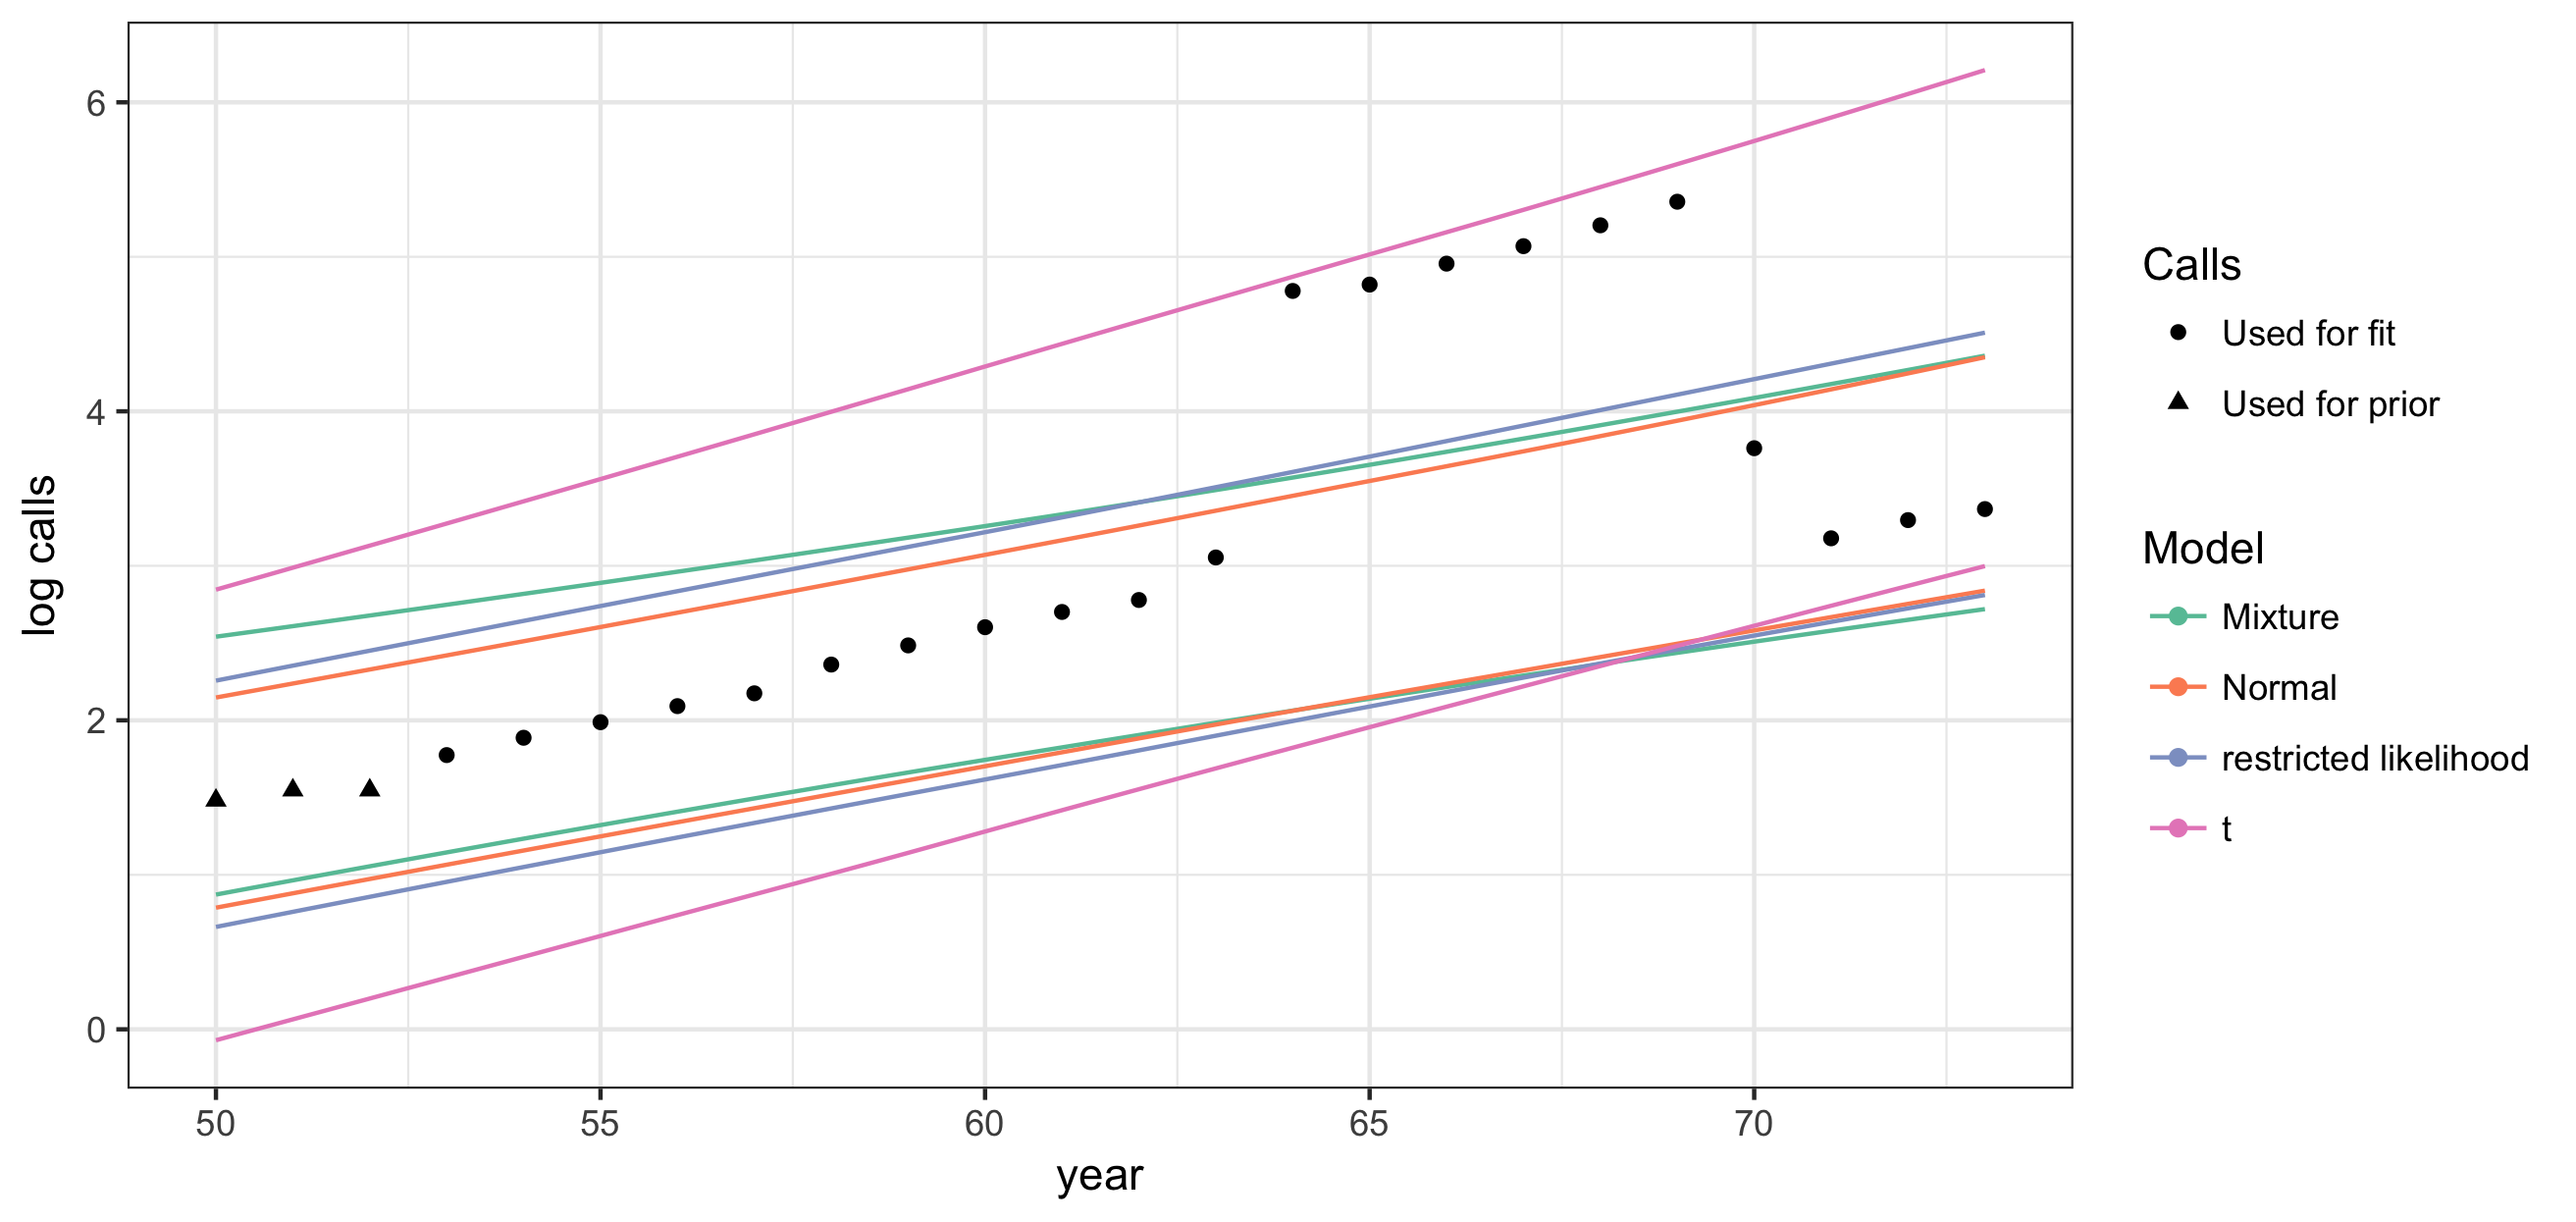
\includegraphics[width = 4in]{figs/calls_predictive.png}}
\caption{Predictive distribution of log(calls) under the Normal theory model fit to the non-outliers, the restricted likelihood model with Tukey's M-estimator for the slope and intercept with Huber's `proposal 2'  for scale, and a heavy-tailed t-distribution model. The first three data points were used to specify the prior with the remaining points used in the posterior fits. See details in the Appendix.}
\label{fig:calls_predictive}
\end{figure}


%
% and the development
%of computational strategies that allow us to truly condition on the observed $T(\by)$ and 
%fit the model in formal Bayesian fashion.  In this work, we focus
%on robustness, and natural choices of $T(\by)$ for the one-sample problem include a set of middling order statistics, a trimmed
%mean, or a classical robust estimator of location and/or scale.  
%We have previously implemented several of these methods and have found them to perform well \citep[][]{lewis2012}. Versions most extensible to the linear model include the M-estimators in the tradition of \cite{huber1964}, least median squares (LMS), and least trimmed squares (LTS). For these choices the restricted likelihood is not available in closed form, making computation of the restricted posterior a challenge. For low-dimensional statistics $T(\by)$ and parameters $\bth$, the direct computational strategies described in \cite{lewis2014} can be used to estimate the incomplete posterior conditioned on essentially any statistic.  These strategies rely on generation of complete data sets from different values of $\bth$.  
%Each complete data set leads to a statistic $T(\by)$ under $\bth$, and these generated statistics are used to estimate the density at $T(\by_{obs})$, where $\by_{obs}$ is the observed complete data. This estimate is fed into Bayes' theorem for the update from prior distribution to posterior distribution.  
%



%\subsection{A first data analysis example} %\textcolor{blue}{ADDED}
%\label{darwinAnalysis}
%Before discussing computational details of finding restricted 
%posteriors, we begin by analyzing a simple example involving
%outliers. The data consists of well known measurements of the \green{passage time} of
%light taken by Simon Newcomb in the late nineteenth century and
%contain two clear outliers on the low end. Details and data are
%available in the R package {\tt MASS} and previous analyses appear in
%\cite{stigler1977}, \cite{chan1980}, and \cite{gelman2004}. Letting
%$y_{i}$ denote the $i^{th}$ coded measurement of the passage time of light, we
%assume $y_{i}\iid N (\beta, \sigma^{2})$ for $i=1,2,\dots, n=66$. The
%parameter $\beta$ can be interpreted as the passage time of light with
%$\sigma^{2}$ representing measurement error. The outliers \green{are a clear indication} %make clear
%that this normal model is misspecified.  \green{Also,} %Another reason for model misspecification is that 
%the measurements are coarse, taking on only
%integer values.  For a Bayesian analysis, we must specify prior
%distributions on the parameters $\bth=(\beta, \sigma)$. For this we
%assume an independent normal -- inverse gamma model. That is,
%$\beta\sim N(\eta, \tau^{2})$ and $\sigma^{2}\sim IG(a, b)$. The
%hyperparameters  are fixed for simplicity and taken to be $\eta=23.6$,
%$\tau=2.04$, $a=5$,  and $b=10$. We note that our computational
%strategy described in Section \ref{highDim} makes it feasible to fit
%more complex model structures. The Bayesian model presented here is a
%special case of the linear model in \eqref{LinearModel} presented below.
%
%As summary statistics for the restricted likelihood methods, we
%consider robust simultaneous M-estimators of location and scale as
%well as LMS (least median squares) and LTS (least trimmed squares) estimators. The simultaneous M-estimators $b(\by)$ and $s(\by)$ of $\beta$ and $\sigma$, respectively, are the solutions to the equations
%\begin{eqnarray}
%\label{Mest}
% \sum_{i=1}^n \psi\left(\frac{y_i - b(\by)}{s(\by)}\right)= & 0 \\
% \sum_{i=1}^n \chi\left(\frac{y_i - b(\by)}{s(\by)}\right)= & 0 . \nonumber 
%\end{eqnarray} 
%For the first equation we consider two $\psi$ functions: Huber's and Tukey's. These are both coupled with Huber's `proposal 2'  for the $\chi$ function in the second equation \citep[for details see][]{huber2009}. Tuning parameters for these functions are set to achieve $95\%$ efficiency under normally distributed data. 
%
%LMS minimizes the median squared residual and LTS minimizes the sum of the $k$ smallest squared residuals where $k$ is chosen by the user. These estimators are considered because, unlike the M-estimators above, they can achieve high breakdown.
%%These estimators are easily implemented by the {\tt rlm} function of the {\tt MASS} package in R. 
%It is well known that LMS has highest possible breakdown but is inefficient. LTS is more efficient and its breakdown properties are determined by $k$, with highest possible breakdown occurring for $\left \lfloor{\frac{n+1}{2}}\right \rfloor\leq k\leq\left \lfloor{\frac{n+2}{2}}\right \rfloor$. %For the current data set $n=66$ and we take $k=34$ to achieve highest possible breakdown. 
%For the current analysis we do not choose $k$ to achieve highest possible breakdown. Instead, with $n=66$ and we choose $k=62$ (roughly $95\%$ of $n$) to be \green{more} %somewhat
%comparable to the tuning parameters chosen for the M-estimators. The LMS and LTS \green{estimators} are also coupled with an estimator of scale for the conditioning. We set the scale estimator to the minimum of the corresponding objective function, appropriately scaled for consistency. %we use the scale estimator corresponding to the respective objective function. These are the median squared residual for LMS and sum of the smallest squared residuals for LTS multiplied by an appropriate correction factor chosen for consistency. %Computation of these estimators are also implemented in the {\tt MASS} package by the function {\tt lqs}.
%
%For comparison to a traditional Bayesian outlier approach we also fit a heavy-tailed model by changing the data distribution from a normal to a Student's $t$ with $\nu=5$ degrees of freedom. We note that the variance of the data under this model is $\frac{\nu}{\nu-2}\sigma^{2}$.  For comparability, it is this quantity that has the prior distribution $IG(a,b)$ given above.   
%
%The marginal posteriors for $\beta$ and $\sigma^{2}$ as well as the
%predictive distribution \eqref{RestrictedpredDist} under each model
%are displayed in Figures
%\ref{fig:newcombBeta}-\ref{fig:newcombPred}. Both of the two small
%outliers and the normal prior on $\beta$ centered at $23.6$ are
%influential in the results. The normal theory model is most
%drastically affected with the posterior of $\beta$ being pulled
%towards the prior and outliers. Inference on $\sigma^{2}$ under this
%model is impacted by the outliers (see Figure
%\ref{fig:newcombSig2}) \green{resulting in overestimation of $\sigma^{2}$}. 
%The heavy-tailed model as well as the
%restricted likelihood methods with LTS, Huber's, and Tukey's summary
%statistics are less influenced by the outliers and priors. The
%marginal posteriors for $\beta$ are closer to the center of the
%non-outlying data. Inference on the variance parameter also more
%closely reflects the variance information in this part of the data
%(the mean and variance of the data without the two outliers are $27.8$
%and $25.8$, respectively). The posterior of $\beta$ under LTS is
%slightly more dispersed than under the two M-estimator methods. This is
%also reflected in the variance parameter in that under LTS the posterior distribution \green{concentrates on 
%slightly larger values of $\sigma^2$} % is slightly higher. 
%While LMS has high breakdown, it has been more drastically affected by the normal prior centered at $23.6$ than the others. This is % likely 
%because LMS achieves high breakdown by discounting much of the information in the data. 
%
%Though inference for the main parameter of interest ($\beta$) is
%similar between the traditional heavy-tailed approach and the new
%method with LTS, Huber's, and Tukey's summary statistics,  the
%traditional heavy-tailed method has the disadvantage of less precise
%predictive capability. This is reflected in the heavier tails of its
%predictive distribution  \eqref{RestrictedpredDist} seen in Figure
%\ref{fig:newcombPred} (plotted are the log predictive \green{densities} %distributions
%under each method). The predictive distributions under each of the
%restricted likelihood methods are comparable. Surprisingly, despite the poor
%inference on $\beta$ under LMS, the predictive distribution is
%\green{concentrated more sharply} than \green{under} the other restricted likelihood methods. This is
%related to its posterior of $\sigma^{2}$ seen in
%Figure \ref{fig:newcombSig2}  which is the tightest
%distribution and shifted the most to the left. 
%% However, this is likely a consequence of the scale estimator chosen for the conditioning. Recall it involves a correction factor which is chosen asymptotically. Even for $n=66$, this correction factor can contribute to underestimation (\textcolor{blue}{REFERENCE: I know I read something like this somewhere}). \red{[I don't know what exactly this correction factor is. Is it similar to the bending constant for $\psi$?]}
%
%%\red{[I suggest to omit the following paragraphs given that the second last paragraph in the previous section (``the key to the productive ...'') has similar discussions already.]} This simple example raises many questions regarding the proposed method. The first of which is how to choose the summary statistic. In principle, we may choose any summary and it doesn't have to be an estimator of location and scale. However, for outlier problems this choice seems logical and we use it for this paper. Further, estimator specific tuning parameters clearly effect the results. For example, we also looked at LTS with $k=34$ to achieve high breakdown. This resulted in a posterior for $\beta$ which closely resembled that of LMS. 
%
%%Other questions may be posed by the reader and addressing each of these is beyond the scope of this paper. Instead we focus on introducing the method and deriving a computational strategy that will allow such models to be fit to higher dimensional problems with a large class of summary statistics. It is our hope that this computational strategy will facilitate the study of further questions regarding the method. 
%
%\begin{sidewaysfigure}
%\centering
%\captionsetup{justification=centering}
%\subcaptionbox{\label{fig:newcombBeta}}{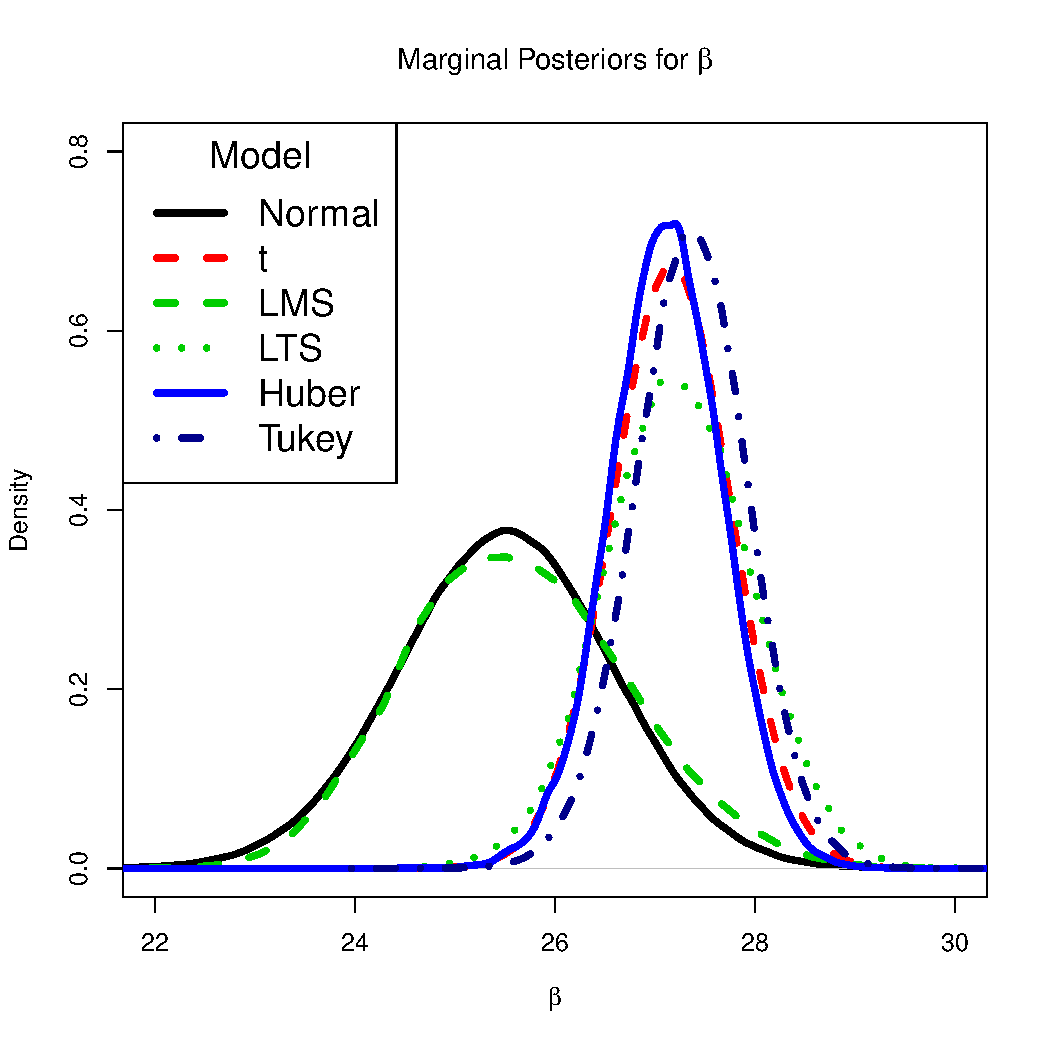
\includegraphics[width=3.4in]{posteriorBetaNewcombDataParamSet2trim_2.pdf}}\quad
%\subcaptionbox{\label{fig:newcombSig2}}{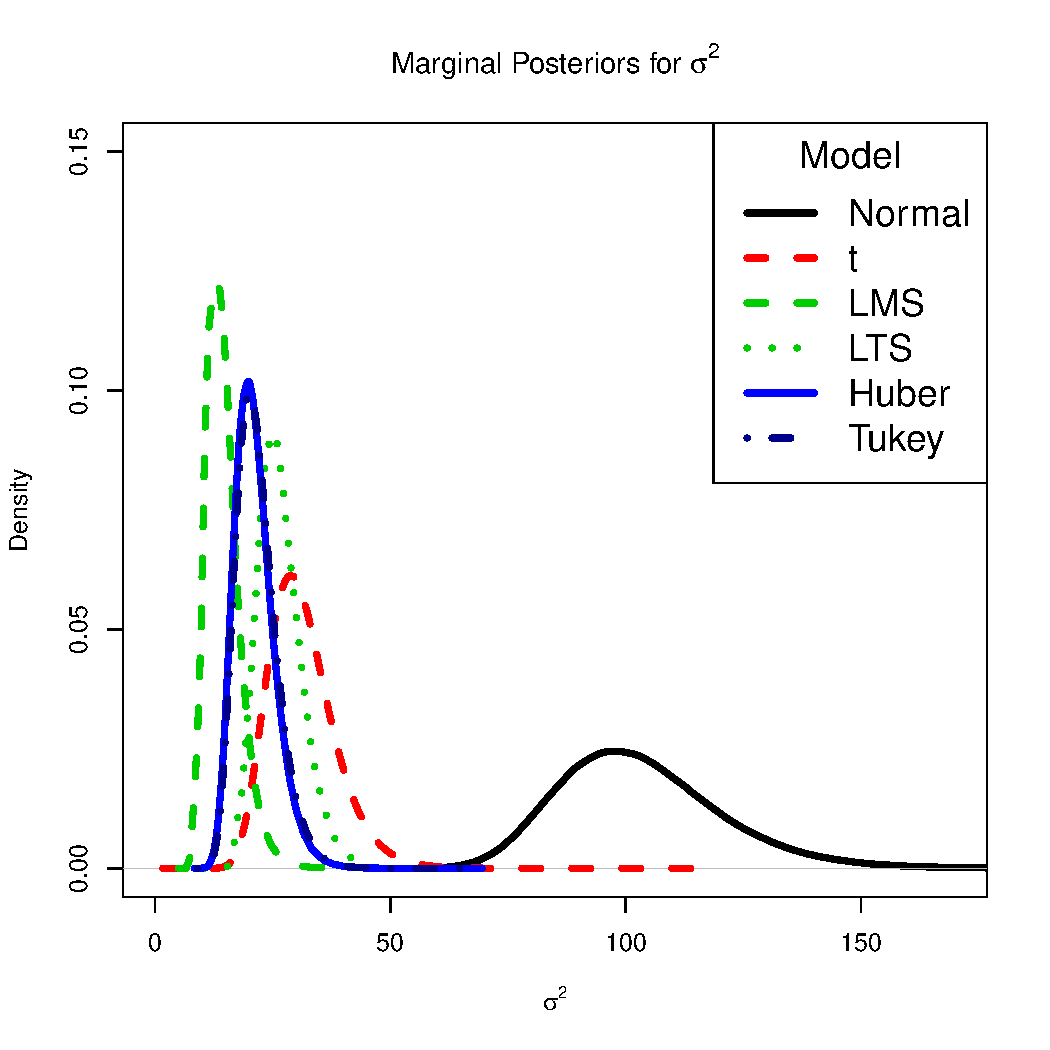
\includegraphics[width=3.4in]{posteriorSigma2NewcombDataParamSet2trim_2.pdf}}\quad
%\subcaptionbox{\label{fig:newcombPred}}{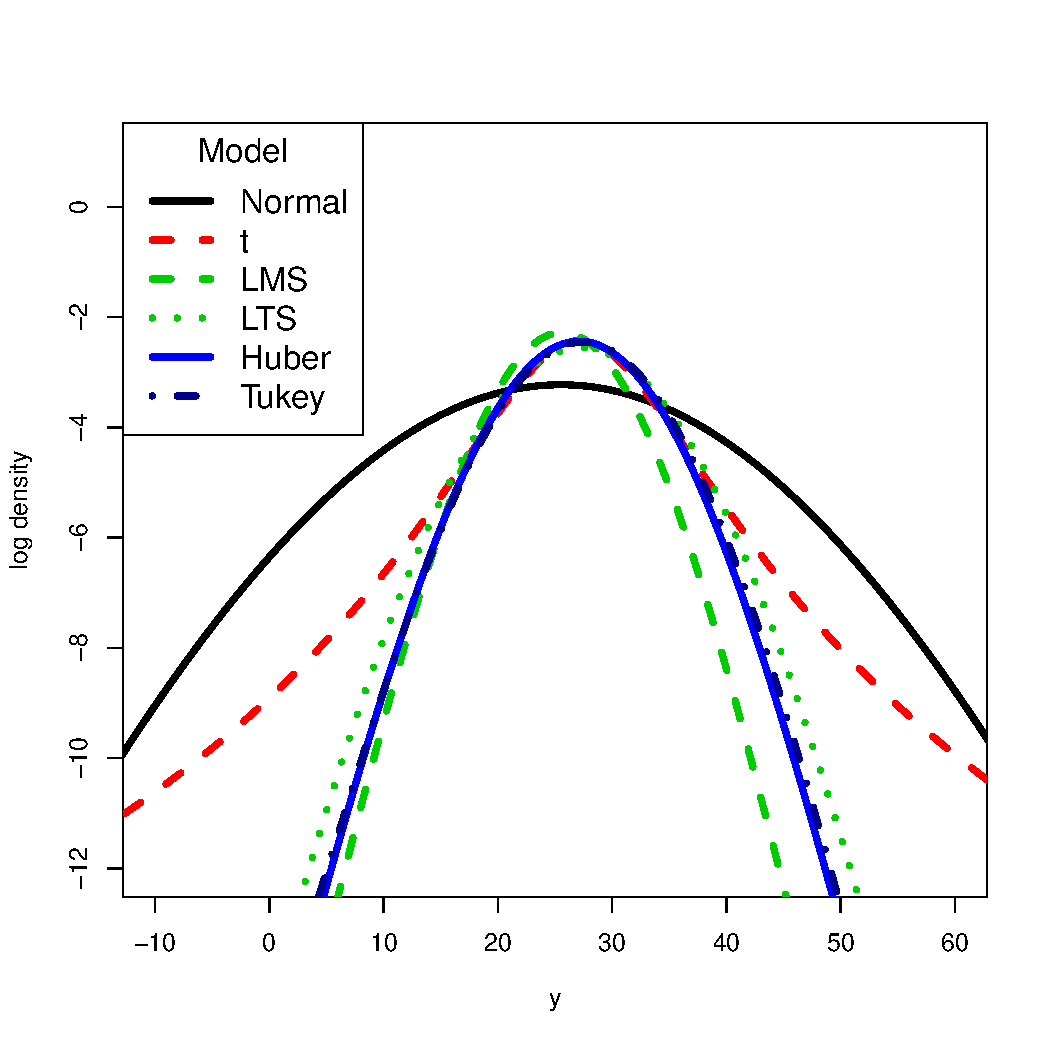
\includegraphics[width=3.4in]{logpredDistParamset2nu5trim_2.pdf}}
%\caption{Clockwise from top left: (a) marginal posteriors of $\beta$ (b) marginal posteriors for $\sigma^{2}$ (c) log predictive distributions.}
%\label{fig:newcomb}
%\end{sidewaysfigure}
%
%
%%\begin{sidewaysfigure}
%%\begin{subfigure}[b]{.5\linewidth}
%%\captionsetup{justification=centering}
%%\centering 
%%\caption{}\label{fig:newcombBeta}
%%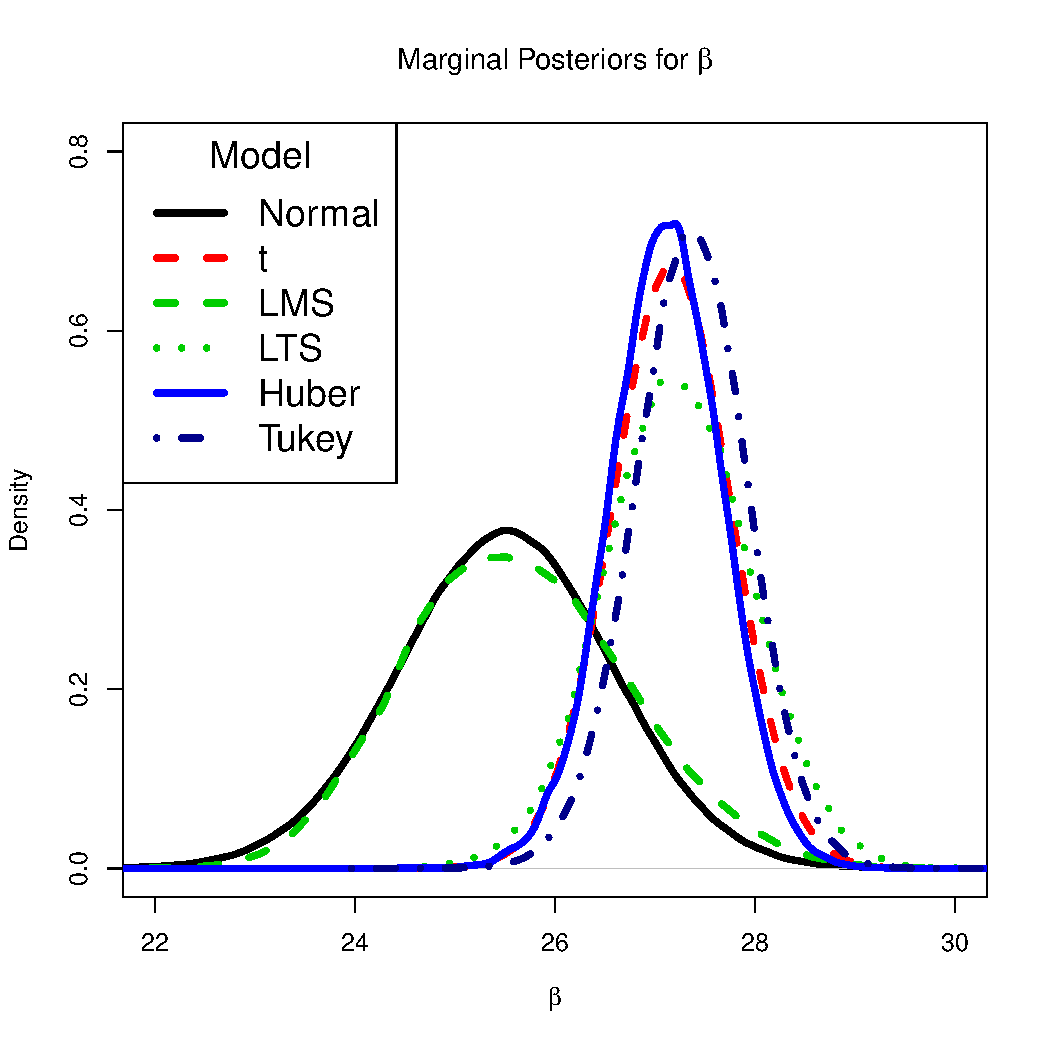
\includegraphics[width=3.4in]{posteriorBetaNewcombDataParamSet2trim_2.pdf}
%%\end{subfigure}
%%\quad
%%\begin{subfigure}[b]{.5\linewidth}
%%\captionsetup{justification=centering}
%%\centering
%%\caption{}\label{fig:newcombSig2}
%%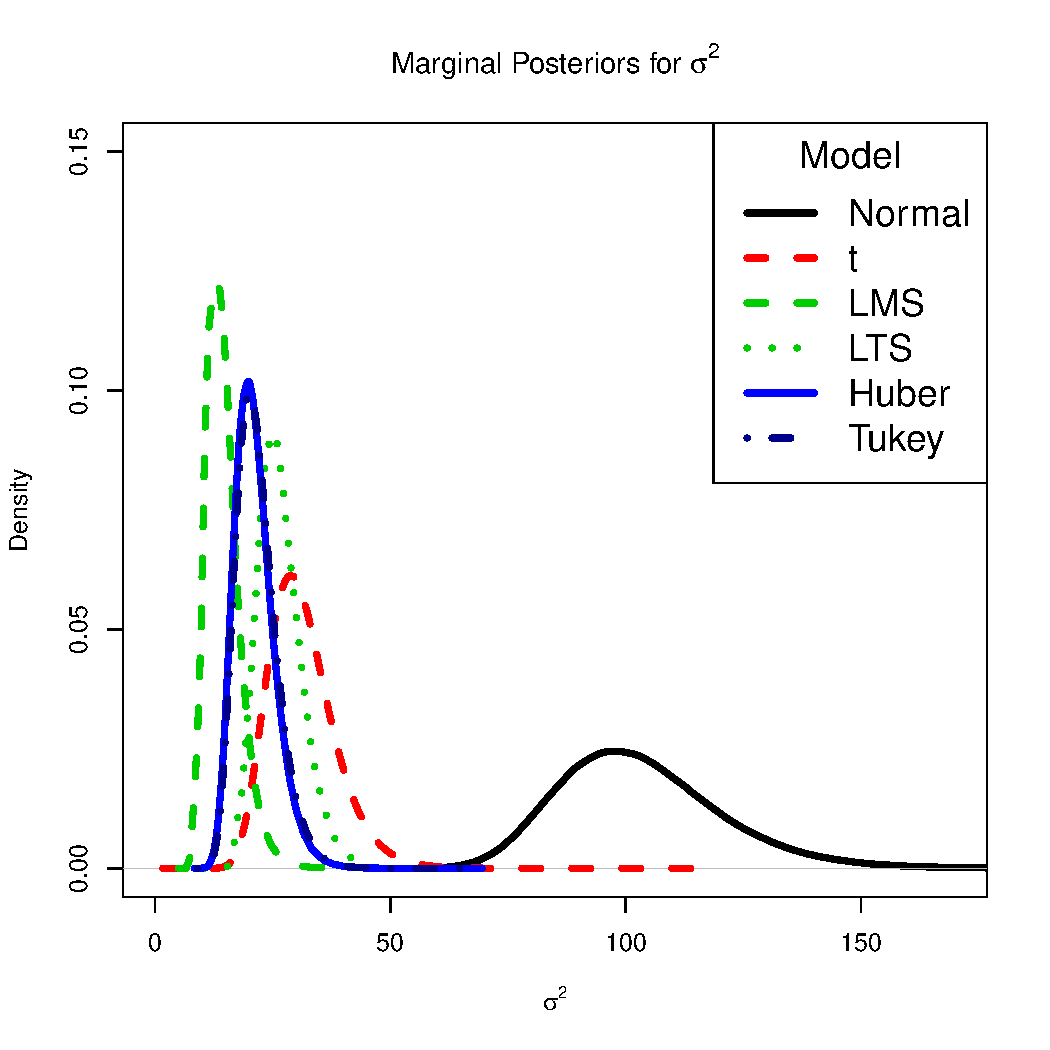
\includegraphics[width=3.4in]{posteriorSigma2NewcombDataParamSet2trim_2.pdf}
%%\end{subfigure}
%%\quad
%%\begin{subfigure}[b]{.5\linewidth}
%%\captionsetup{justification=centering}
%%\centering
%%\caption{}\label{fig:newcombPred}
%%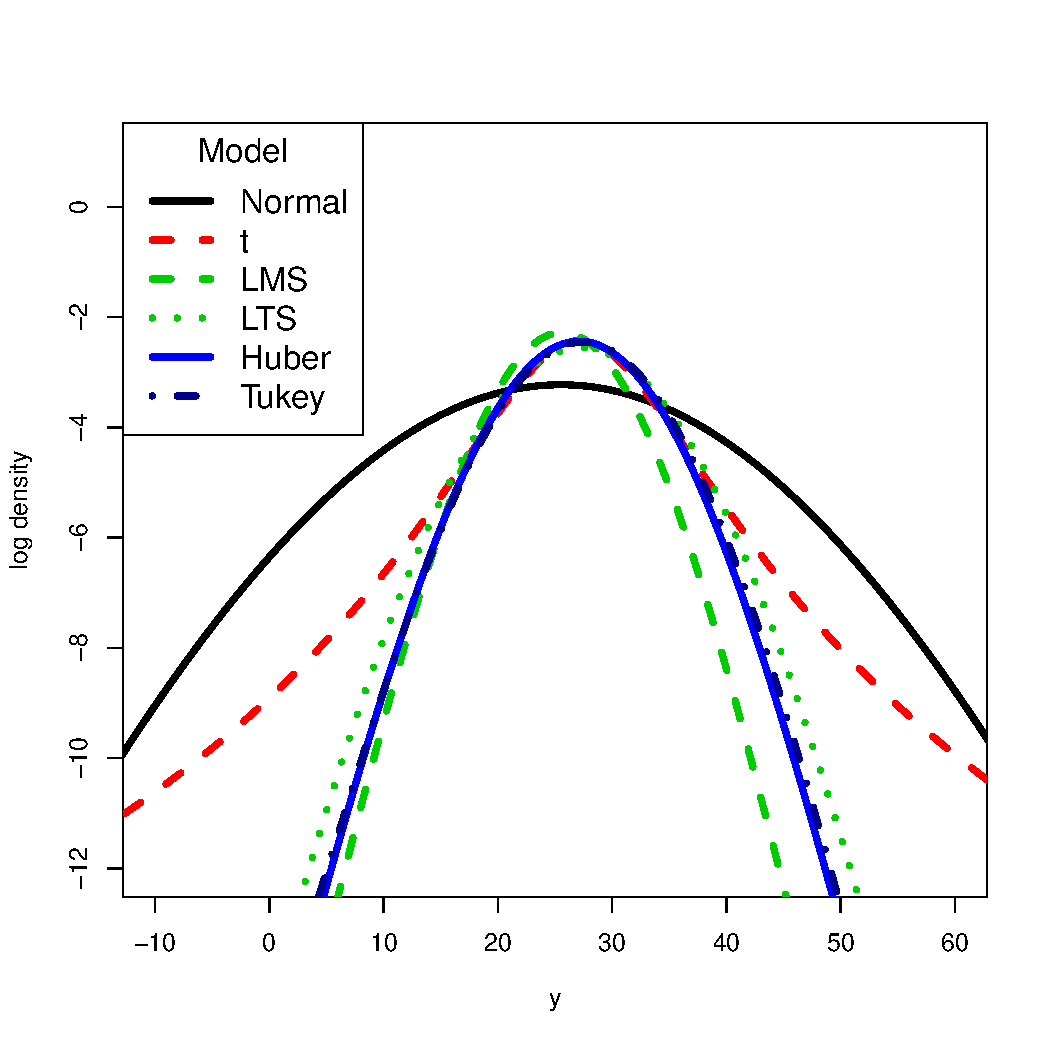
\includegraphics[width=3.4in]{logpredDistParamset2nu5trim_2.pdf}
%%\end{subfigure}
%
%%\caption{Clockwise from top left: (a) marginal posteriors of $\beta$. (b) marginal posteriors for $\sigma^{2}$. (c) log predictive distributions.}
%%\label{fig:newcomb}
%%\end{sidewaysfigure}
%
%
%
%%\textcolor{blue}{if we add the Newcomb and Belgium Calls data examples, this might be a good place to add them because they are low dimensional. I think it would be a good lead into the high dimensional computational strategies}
%
%

\section{Restricted Likelihood for the Linear Model}
\label{BayesLinMod}

The simple examples in the previous section highlight that productive use of the restricted likelihood relies on a good choice of $T(\by)$. This work focuses on robustness in linear models where natural choices include many used above:  M-estimators in the tradition of \cite{huber1964}, least median squares (LMS), and least trimmed squares (LTS). For these choices the restricted likelihood is not available in closed form, making computation of the restricted posterior a challenge. For low-dimensional statistics $T(\by)$ and parameters $\bth$, direct computational strategies described in \cite{lewis2014} can be used to estimate the restricted posterior conditioned on essentially any statistic.  These strategies rely on density estimation $f(T(\by)|\theta)$ using samples of $T(\by)$ for many values of $\theta$; a strategy which breaks down in higher dimensions. This section outlines a data-augmented MCMC algorithm that can be applied to the Bayesian linear model when $T(\by)$ consists of estimates of the regression coefficients and scale parameter. 

\subsection{The Bayesian linear model}
We focus on the use of restricted likelihood for the Bayesian linear
model with a standard formulation: 
%\begin{eqnarray}
%\label{LinearModel}
%\bbeta & \sim & \pi_1(\bbeta); \qquad \sigma^2  \sim  \pi_2(\sigma^2)
%\nonumber\\
%y_i  & =  & x_i^\top \bbeta + \epsilon_i , \mbox{ for } i = 1, \ldots, n 
%\end{eqnarray}
\begin{eqnarray}
\label{LinearModel}
\bth&=&(\bbeta,\sigma^2) \sim  \pi(\bth) 
\nonumber\\
y_i  & =  & x_i^\top \bbeta + \epsilon_i , \mbox{ for } i = 1, \ldots, n 
\end{eqnarray}
where $x_i$ and $\bbeta \in \mathbb{R}^p$, $\sigma^2 \in \mathbb{R}^+$, 
and the $\epsilon_i$ are independent draws from a distribution with center $0$ and scale $\sigma$. $X$ denotes the design matrix whose rows are  $x_i^\top$. 

For the restricted likelihood model,  conditioning statistics are assumed to be of the form $T(\by) = (\bb(X, \by), s(X, \by))$ where $\bb(X, \by)= (b_1(X,\by), \dots,b_p(X,\by))^\top\in \mathbb R^{p}$ is an estimator for the regression coefficients and $s(X, \by)\in \{0\} \cup {\mathbb R}^+$ is an estimator of the scale. Throughout, observed data and summary statistic is denoted by $\by_{obs}$ and $T(\by_{obs})=(\bb(X, \by_{obs}), s(X, \by_{obs}))$, respectively. 
% In particular, we demonstrate the method using simultaneous M-estimators defined by \eqref{Mest} for the one-sample setting and easily extended to the linear model in \eqref{LinearModel}. The estimator of the \green{regression} coefficients is denoted by $\bb(X, \by)\in \mathbb R^{p}$ and that of the scale by \green{\sout{$s(X, \by)\in \mathbb R$} $s(X, \by)\in \{0\} \cup {\mathbb R}^+$} . Thus, $T(\by)=(\bb(X, \by), s(X, \by))$. 
Several conditions are imposed on the model and statistic to ensure validity of the MCMC algorithm:
\begin{itemize}
\labitem{C1}{fullRank} The $n \times p$ design matrix, $X$, whose $i^{th}$ row is $x_i^\top$, 
is of full column rank.  
\labitem{C2}{supReal} The $\epsilon_i$ are a random sample from some distribution which has a density with 
respect to Lebesgue measure on the real line and for which the support is the real line.  
\labitem{C3}{asb}$\bb(X,\by)$ is almost surely continuous and differentiable with respect to $\by$.  
\labitem{C4}{as} $s(X,\by)$ is almost surely positive, continuous, and differentiable with respect to $\by$.  
\labitem{C5}{regEq} $\bb(X,\by+X\bv)=\bb(X,\by)+\bv \ \ \text{for  all}\ \bv\in\mathbb{R}^p$. 
\labitem{C6}{scaleEqReg} $\bb(X,a\by)=a\bb(X,\by)\ \ \ \text{for all constants } a$.  
\labitem{C7}{regIn} $s(X,\by+X\bv)=s(X,\by) \ \ \text{for all}\ \bv\in\mathbb{R}^p$.  
\labitem{C8}{scaleEq2Reg} $s(X, a\by)=|a|s(X,\by) \ \ \text{for all constants } a$.  
\end{itemize}
Properties \ref{regEq} and \ref{scaleEqReg} of $\bb$ are called
\textit{regression} and \textit{scale equivariance},
respectively.  Properties \ref{regIn} and \ref{scaleEq2Reg} of $s$ are called \textit{regression invariance}
and \textit{scale equivariance}. 
Many estimators satisfy the above properties, including simultaneous M-estimators \citep{huber2009, maronna2006} for which the R package \texttt{brlm} (\texttt{github.com/jrlewi/brlm}) is available to implement the MCMC described here. Further software development is required to extend the MCMC implementation beyond these M-estimators. The package also implements the direct computational methods described in \cite{lewis2014}. These methods are effective in lower dimensional problems and were used in several of the examples in Section \ref{illustrations}.

%The strategy described in the previous paragraph extends to full-blown regression models.  Robust regression methods lead naturally to a conditioning statistic in the form of a classical M-estimator for $\bbeta$
%and a companion estimator for $\sigma$.  We denote the resulting estimator which involves the covariates through
%the design matrix and the response 
%as $T(\by) = (\bb(X,\by), s(X,\by))$, with $\bb(X,\by) = (b_1(X,\by), \cdots,
%b_p(X,\by))^\top$.  Simultaneous M-estimators have a number of standard properties \ref{asb}-\ref{scaleEq2Reg} which
%prove useful in the sequel \citep{huber2009, maronna2006}.  
%\begin{itemize}
%\labitem{C3}{asb}$\bb(X,\by)$ is almost surely continuous and differentiable with respect to $\by$.  
%\labitem{C4}{as} $s(X,\by)$ is almost surely positive, continuous, and differentiable with respect to $\by$.  
%\labitem{C5}{regEq} $\bb(X,\by+X\bv)=\bb(X,\by)+\bv \ \ \text{for  all}\ \bv\in\mathbb{R}^p$. 
%\labitem{C6}{scaleEqReg} $\bb(X,a\by)=a\bb(X,\by)\ \ \ \text{for all constants } a$.  
%\labitem{C7}{regIn} $s(X,\by+X\bv)=s(X,\by) \ \ \text{for all}\ \bv\in\mathbb{R}^p$.  
%\labitem{C8}{scaleEq2Reg} $s(X, a\by)=|a|s(X,\by) \ \ \text{for all constants } a$.  
%\end{itemize}

%Properties \ref{regEq} and \ref{scaleEqReg} of $\bb$ are called
%\textit{regression} and \textit{scale equivariance},
%respectively.  Properties \ref{regIn} and \ref{scaleEq2Reg} of $s$ are called \textit{regression invariance}
%and \textit{scale equivariance}. 
%Many other estimators satisfy these properties, and our subsequent results apply equally
%well to them.  With more cumbersome statements, the upcoming results can be adjusted to handle 
%a relaxation of \ref{as} that 
%$s(X,\by_{obs}) > 0$ and $P(s(X,\by)>0)>0$.  
%

%\textcolor{blue}{commented out `Both conditions can be relaxed, although this would necessitate restating several later results.' and the paragraph here starting with `in the sequel'}
%In the sequel, we specifically consider both normal and $t$ distributions with
%mean $0$ and variance $\sigma^2$ for the $\epsilon_i$ 
%but note that our methods apply much more widely.  The prior distributions $\pi_1$ and $\pi_2$ can take
%many forms and may be joined to form a joint distribution for non-independent $\bbeta$
%and $\sigma^2$.  The conditionally conjugate normal/inverse gamma pair is a common 
%choice.  
%The methods we develop apply to the linear model in \eqref{LinearModel} and to many variations
%on it. For example, the prior distributions $\pi_1$ and $\pi_2$ can be joined to form a joint distribution for non-independent $\bbeta$
%and $\sigma^2$. 
%
%
%As summary statistics for the data, we concentrate on robust estimators for the 
%\green{regression} coefficients in the linear model and an associated 
%estimator of the scale. In particular, we demonstrate the method using simultaneous M-estimators defined by \eqref{Mest} for the one-sample setting and easily extended to the linear model in \eqref{LinearModel}. The estimator of the \green{regression} coefficients is denoted by $\bb(X, \by)\in \mathbb R^{p}$ and that of the scale by \green{\sout{$s(X, \by)\in \mathbb R$} $s(X, \by)\in \{0\} \cup {\mathbb R}^+$} . Thus, $T(\by)=(\bb(X, \by), s(X, \by))$. The observed complete data is denoted by $\by_{obs}$ with observed statistic  denoted by $T(\by_{obs})=(\bb(X, \by_{obs}), s(X, \by_{obs}))$. 


%Assumption \ref{supReal} is important as it translates into a continuous distribution for $\bb(X, \by)$ and $s(X, \by)$ (with respect to $\by$), which is presumed for our computational strategy described below. The full column rank assumption \ref{fullRank} is made apparent by an examination of the proofs in the the appendix. 

%These estimates convey information about $\bth=(\bbeta,\sigma)$
%while downweighting outliers.  The M-estimator of $\bbeta$ is determined by a $\rho$ function through the minimization
%\begin{eqnarray}
%\label{Mest}
%\bb(X,\by) & = & \argmin_{\bbeta} \sum_{i=1}^n \rho\left(\frac{y_i - x_i^\top \bbeta}{\sigma}\right) .  
%\end{eqnarray} 
%The scale estimator $s(X,\by)$ is determined simultaneously as another M-estimator or is determined through
%a separate calculation, for example the mean-absolute-deviation from an $\ell_1$ regression fit. Other estimators for the coefficients considered are least median squares (LMS) and least trimmed squares (LTS). LMS minimizes the median squared residual and LTS minimizes the sum of the $k$ smallest squared residuals where $k$ is chosen by the user. These estimators are also coupled with a scale estimator.% that is determined by the objective function evaluated at the minimum, appropriately scaled by a correction factor for consistency. 

%which is presumed for our computational strategy. %Before deriving this strategy in section \ref{highDim}, we demonstrate the utility of the incomplete likelihood with a simple location and scale example. %The results we derive also apply to other estimators satisfying conditions \ref{asb}-\ref{scaleEq2Reg} below, not just M-estimators.   



\subsection{Computational strategy}
\label{highDim}
%For low-dimensional statistics $T(\by)$ and $\bth$, the direct computational strategies described in \cite{lewis2014} can be used to evaluate the incomplete likelihood posterior.  
%These strategies rely on generation of complete data sets from different values of $\bth$.  
%Each complete data set leads to a statistic $T(\by)$ under $\bth$, and these generated statistics are used to estimate the density at $T(\by_{obs})$, where $\by_{obs}$ is the observed complete data. This estimate is fed into Bayes' theorem for the update from prior distribution to posterior distribution.  For the example in the previous section, these strategies work well.
%\textcolor{blue}{Comment out `A variety of  variance reduction techniques which exploit\dots' because it seemed too vague and a bit off topic}
%A variety of  variance reduction techniques which exploit 
%properties of the distribution of $\by$ 
%improve the performance of these strategies.  

%As mentioned above, direct computational strategies designed to approximate the restricted posterior break down for high-dimensional statistics $T(\by)$ or high-dimensional parameters $\bth$. %, direct computational strategies break down.  When the conditioning statistic is of high-dimension, density estimation becomes difficult and the associated approximate update in (\ref{RestrictedPosterior}) is unstable; when $\bth$is high dimensional, grid-based calculation and other numerical integration strategies fail.  
%However, Markov chain Monte Carlo (MCMC) methods were developed for exactly these situations.  We turn to MCMC to 
%fit the model in these circumstances.  

%The general style of algorithm that we present relies on the decomposition of the sampling density in (\ref{FullLikelihood})
%into one piece involving only $T(\by)$ and a second piece for the
%complete data $\by$ given $T(\by)$. 
%Relying on the modularity of MCMC algorithms, we construct a data augmented Gibbs sampler targeting $\pi(\bth, \by | T(\by)=T(\by_{obs}))$, the joint posterior of $\bth$ and $\by$ conditioned on the summary statistic $T(\by_{obs})$ for observed data vector $\by_{obs}$. The Gibbs sampler iteratively samples from the full conditionals written as $\pi(\bth|\by T(\by)=T(\by_{obs})$ and $f(\by|\bth, T(\by)=T(\by_{obs})$
% \textcolor{blue}{some major changes from here to the end of the section}
The general style of algorithm we present is a data augmented
MCMC targeting $f(\bth, \by |
T(\by)=T(\by_{obs}))$, the joint distribution of $\bth$ and the full
data given the summary statistic $T(\by_{obs})$. 
 The Gibbs sampler \citep{gelfand1990} iteratively samples from the
 full conditionals 1) $\pi(\bth|\by, T(\by)=T(\by_{obs}))$ and 2) $f(\by|\bth, T(\by)=T(\by_{obs}))$.  When $\by$ has the summary statistic $T(\by) = T(\by_{obs})$,
the first full conditional is the same as the full data posterior $\pi(\bth|\by)$. In this case, the condition $T(\by) = T(\by_{obs})$ is redundant.  This allows us to make use of conventional MCMC steps for this generation.  For typical regression models, algorithms abound. Details of the recommended algorithms depend on details of
the prior distribution and sampling density and we assume this can be done \citep[see e.g.,][]{liu1994, liang2008}.  

%As examples, a normal
%prior distribution and normal likelihood in the regression setting
%allow one to alternate conditional generations of $\sigma^2$ and $\bbeta$, and blocking the generation of $\bbeta$ generally
%leads to quicker convergence and mixing \citep{liu1994}; a thick-tailed scale mixture of normal distributions
%in the style of the hyper-$g/n$ prior \citep{liang2008} necessitates an additional stage for the sampler where the scale 
%$g/n$ is generated; a thick-tailed sampling density such as a $t$ distribution can be handled with the addition of 
%a scale parameter for each case and an extra stage where these scale parameters are generated.  

%\green{Alternative algorithms substitute other generations for the full conditionals, such as the Metropolis-Hastings propose and accept/reject framework.  Our algorithms are based on the decomposition of the MCMC algorithm into conventional full data sampling steps where $\bth$ is generated given $\by$, and steps that allow us to complete the data set where $\by$ is generated given $\bth$ and $T(\by)$.  The latter generation relies on the conditioning set $\mathcal{A}=\{\by\in \mathbb{R}^n|T(\by)=T(\by_{obs})\}$.  The set $\mathcal{A}$ may contain more than one element (i.e., it is not degenerate) when $T(\by) : \by \rightarrow T(\by)$ is not a $1-1$ function.}

%The other stage in the Gibbs sampler is the generation of complete data from the full conditional  $f(\by|\bth, T(\by)=T(\by_{obs}))$. %Condition \ref{supReal} above facilitates the extension of convergence proofs for the complete data algorithm to those for the incomplete data algorithm.  
%In this subsection, we focus exclusively this stage. 
%we begin with any conventional complete data algorithm.  In the case of typical regression models, these algorithms abound.  Details of the algorithm depend on details of
%the prior distribution and sampling density.  As examples, a normal
%prior distribution and normal likelihood in the regression setting
%allow one to alternate conditional generations of $\sigma^2$ and $\bbeta$, and blocking the generation of $\bbeta$ generally
%leads to quicker convergence and mixing \citep{liu1994}; a thick-tailed scale mixture of normal distributions
%in the style of the 
%hyper-$g/n$ prior \citep{liang2008} necessitates an additional stage for the sampler where the scale 
%$g/n$ is generated; a thick-tailed sampling density such as a $t$ distribution can be handled with the addition of 
%a scale parameter for each case and an extra stage where these scale parameters are generated.  
%The additional stage needed to implement the incomplete likelihood analysis via MCMC 
%is a generation of the complete data given statistic ($T(\by_{obs})$) and parameter ($\bth$).  Condition \ref{supReal} facilitates the extension of convergence proofs for the complete data algorithm to those for the incomplete data algorithm.  
%In this subsection, we focus exclusively on the additional stage
%where we generate $\by | \bth, T(\by)$.  
For a typical model and conditioning statistic, the second full conditional $f(\by|\bth, T(\by)=T(\by_{obs}))$ %\blue{ =f(\by|\bth, \by\in\mc A)}$ 
is not available in closed form.  We turn to Metropolis-Hastings \citep{hastings1970},
using the strategy of proposing full data $\by \in \mathcal{A}:=\{\by \in \mathbb{R}^n | T(\by)=T(\by_{obs})\}$ from a well defined distribution with support $\mathcal{A}$ and either accepting or rejecting the
proposal. Let $\by_p, \by_c \in \mathcal{A}$ represent the proposed and current
full data, respectively. Denote the proposal distribution for $\by_{p}$ by $p(\by_p|\bth,T(\by_p) = T(\by_{obs})) = p(\by_p|\bth,\by_p \in \mathcal{A}) = p(\by_p | \bth)$.  The last equality follows from the fact that our $p(\cdot | \bth)$ assigns probability one to the event $\{ \by_p \in \mathcal{A} \}$.  These equalities still hold if the dummy argument $\by_p$ is replaced with $\by_c$.  The conditional density is
\begin{eqnarray*}
f(\by | \bth, \by \in \mathcal{A}) =  \frac{f(\by | \bth) I(\by \in \mathcal{A} | \by, \bth)}{\int_\mathcal{A} f(\by | \bth) d\by} 
      = \frac{f(\by | \bth)}{\int_\mathcal{A} f(\by | \bth) d\by} 
\end{eqnarray*}
for $\by \in \mathcal{A}$.  This includes both $\by_p$ and $\by_c$.  The Metropolis-Hastings acceptance probability  is the minimum of 1 and $R$ where,
\begin{eqnarray}
\label{MHRatio}
R & = & \frac{f(\by_p|\bth,\by_p \in \mathcal{A})}{f(\by_c|\bth,\by_c \in \mathcal{A})}  
                \frac{p(\by_c|\bth, \by_c \in \mathcal{A})}{p(\by_p|\bth,\by_p \in \mathcal{A})} \\
  & = & \frac{f(\by_p | \bth)}{\int_\mathcal{A} f(\by | \bth) d\by} \frac{\int_\mathcal{A} f(\by | \bth) d\by}{f(\by_c | \bth)} \frac{p(\by_c | \bth)}{p(\by_p | \bth)} \\
 & = & \frac{f(\by_p|\bth)}{f(\by_c|\bth)} \frac{p(\by_c|\bth)}{p(\by_p|\bth)} .  
\end{eqnarray}
%In the above expression, the second line follows from the first for
%the following reason. The proposed \green{vector $\by$} is sampled from
%  $\mathcal{A}$ so that
%$T(\by_{p})=T(\by_{c})=T(\by_{obs})$. This implies 
%\green{\sout{$f(\by |\bth,
%T(\by)=T(\by_{obs}))=f(\by |\bth)\pi(\bth)/\red{f[?]}\pi(\bth, T(\by)=T(\by_{obs}))$}
%\begin{eqnarray}
%f(\by |\bth,\by \in \mathcal{A})) & = & \frac{f(\by | \bth) \pi(\bth) I(\by \in \mathcal{A})}{\int f(\by | \bth) \pi(\bth) I(\by \in \mathcal{A}) d\bth}
%\end{eqnarray}}
%where $\by$ represents either $\by_{p}$ or $\by_{c}$. %Further, the expressions $\pi(\bth)$ and $\red{f[?]}\pi(\bth, T(\by)=T(\by_{obs}))$ 
%\green{The expressions $\pi(\bth)$ and $\int f(\by | \bth) \pi(\bth) I(\by \in \mathcal{A})  d\bth$} are the same for $\by_{p}$ and $\by_{c}$ and cancel in the ratio. %Similar expansions can be made for the proposal distribution. 
%\green{Further, the indicator functions can be dropped since $\by_p$ and $\by_c$ will both fall in $\mathcal{A}$.}  
%\green{Note:  Check this argument carefully}
For the models we consider, evaluation of $f(\by | \bth)$ is straightforward.  Therefore, the difficulty in implementing this Metropolis-Hastings step manifests  itself in the ability to both simulate from and evaluate $p(\by_p | \bth)$; the well defined distribution with support $\mathcal{A}$. We now discuss such an implementation method for the linear model in \eqref{LinearModel}.

\subsubsection{Construction of the proposal}
%\textcolor{blue}{some major revisions as indicated in the responseToReferees}
Our computational strategy relies on proposing $\by$ such that $T(\by) = T(\by_{obs})$ where $T(\cdot) = (\bb(X, \cdot), s(X, \cdot))$ satisfies the conditions \ref{asb}-\ref{scaleEq2Reg}. It is not a simple matter to do this directly, but with the specified conditions, it is possible to scale and shift any $\bz^{*}$ which generates 
a positive scale estimate to such a $\by$ via the following Theorem, whose proof is in the appendix. 
\begin{theorem}
\label{Transformation}
Assume that conditions \ref{as}-\ref{scaleEq2Reg} hold.  Then, any vector $\bz^* \in \mathbb{R}^n$ with conditioning statistic
$T(\bz^*)$ for which $s(X,\bz^*) > 0$ can be transformed into $\by$ with conditioning statistic $T(\by) = T(\by_{obs})$ 
through the transformation 
\[
\by = h(\bz^*) := \frac{s(X,\by_{obs})}{s(X,\bz^*)} \bz^* + X\left(\bb(X,\by_{obs}) - \bb(X,\frac{s(X,\by_{obs})}{s(X,\bz^*)} \bz^*)\right) .  
\]
\end{theorem}% (details are given in Theorem \ref{Transformation} below). Hence, to obtain $\by \in\mathcal A$, we proceed in two steps:
%\begin{enumerate}
%\item Sample $\bz^*\in \mathbb{R}^{n}$ from a known distribution (examples of which are described later).
%\item Transform $\bz^*$ to $\by =h(\bz^*)$ using Theorem \ref{Transformation} so that $T(\by)=T(\by_{obs})$. 
%\end{enumerate}
% To 
%obtain data $\by$ for which $T(\by) = T(\by_{obs})$, we proceed in two
%steps.  
%First, a vector $\bz^*$ is generated from a simple manifold with known
%density, for example, a uniform distribution
%on the surface of the unit sphere in ${\mathbb R}^{n-1}$ (alternatively from
%the model with current values of $\beta$ and $\sigma$).  This leads to 
%$T(\bz^*) = (b(X,\bz^*), s(X,\bz^*))$.  The vector $\bz^*$ is mapped into a vector
%$\by$ by rescaling and shifting appropriately to match the observed conditioning statistic.  For typical estimators, the appropriate scaling is 
%$s(X,\by_{obs}) / s(X,\bz^*)$ with the shift trailing along as needed to match $b(X,\by_{obs})$.  
%To evaluate the proposal density of $\by$,
%we need to adjust the density of $\bz^*$ with a Jacobian.  In the sequel, we use this artificially low-dimensional
%example to illustrate the method.  
%The strategy described in the previous paragraph extends to full-blown regression models.  Robust regression methods lead naturally to a conditioning statistic in the form of a classical M-estimator for $\bbeta$
%and a companion estimator for $\sigma$.  We denote the resulting estimator which involves the covariates through
%the design matrix and the response 
%as $T(\by) = (\bb(X,\by), s(X,\by))$, with $\bb(X,\by) = (b_1(X,\by), \cdots,
%b_p(X,\by))^\top$.  Simultaneous M-estimators have a number of standard properties \ref{asb}-\ref{scaleEq2Reg} which
%prove useful in the sequel \citep{huber2009, maronna2006}.  
%\begin{itemize}
%\labitem{C3}{asb}$\bb(X,\by)$ is almost surely continuous and differentiable with respect to $\by$.  
%\labitem{C4}{as} $s(X,\by)$ is almost surely positive, continuous, and differentiable with respect to $\by$.  
%\labitem{C5}{regEq} $\bb(X,\by+X\bv)=\bb(X,\by)+\bv \ \ \text{for  all}\ \bv\in\mathbb{R}^p$. 
%\labitem{C6}{scaleEqReg} $\bb(X,a\by)=a\bb(X,\by)\ \ \ \text{for all constants } a$.  
%\labitem{C7}{regIn} $s(X,\by+X\bv)=s(X,\by) \ \ \text{for all}\ \bv\in\mathbb{R}^p$.  
%\labitem{C8}{scaleEq2Reg} $s(X, a\by)=|a|s(X,\by) \ \ \text{for all constants } a$.  
%\end{itemize}
%Properties \ref{regEq} and \ref{scaleEqReg} of $\bb$ are called
%\textit{regression} and \textit{scale equivariance},
%respectively.  Properties \ref{regIn} and \ref{scaleEq2Reg} of $s$ are called \textit{regression invariance}
%and \textit{scale equivariance}. 
%Many other estimators satisfy these properties, and our subsequent results apply equally
%well to them.  With more cumbersome statements, the upcoming results can be adjusted to handle 
%a relaxation of \ref{as} that 
%%$s(X,\by_{obs}) > 0$ and $P(s(X,\by)>0)>0$.  
%To understand the Jacobian calculation, we start with the following Theorem whose proof is in the appendix. 
%%We have stated that any vector $\bz^{*} \in \mathbb{R}^n$ can be transformed to a proposal
%%$\by$ satisfying $T(\by) = T(\by_{obs})$.  The properties above ensure
%%that this can be done through the mechanism presented in the following theorem.  The proof of this and other results appear in the appendix.
%\begin{theorem}
%\label{Transformation}
%Assume that conditions \ref{as}-\ref{scaleEq2Reg} hold.  Then, any vector $\bz^* \in \mathbb{R}^n$ with conditioning statistic
%$T(\bz^*)$ for which $s(X,\bz^*) > 0$ can be transformed into $\by$ with conditioning statistic $T(\by) = T(\by_{obs})$ 
%through the transformation 
%\[
%\by = h(\bz^*) := \frac{s(X,\by_{obs})}{s(X,\bz^*)} \bz^* + X\left(\bb(X,\by_{obs}) - \bb(X,\frac{s(X,\by_{obs})}{s(X,\bz^*)} \bz^*)\right) .  
%\]
%\end{theorem}
Using the theorem, the general idea is to first start with an initial vector $\bz^*$ drawn from a known distribution, say $p(\bz^*)$, and transform via $h(\cdot)$ to $\by \in \mathcal{A}$. The proposal density $p(\by|\bth)$ is then a change-of-variables adjustment on $p(\bz^*)$ derived from $h(\cdot)$.
%To evaluate the proposal density $p(\by|\bth)$, we need to adjust the known density of $\bz^*$, $p(\bz^*)$, with the Jacobian of the transformation $h(\cdot)$ to $\by$. We choose the
%distribution of $\bz^*$ to have support on a subset of $\mathbb R^n$ so that
%the transformation to $\by$ is one-to-one and the Jacobian, $\displaystyle \left|\frac{\partial h^{-1}(\by)}{\partial \by}\right|$, can be computed directly.  
In general however, the mapping $h(\cdot)$ is many-to-one: for any $\bv\in \mathbb{R}^{n}$ and any $c\in \mathbb{R}^{+}$, $c\bz^{*} + X\bv$ map to the same $\by$. This makes the change-of-variables adjustment difficult.
%The set $\mathcal{A}$ typically does not lie in a linear space of dimension $n - p - 1$, and 
%so we must account for both the many-to-one nature of the mapping $h(\dot)$ and
%a Jacobian when deriving the proposal density.  
We handle this point by first noticing that the set $\mathcal{A}$ is an $n - p - 1$ dimensional space:  there are $p$ constraints imposed by the regression coefficients and one further constraint imposed by the scale. Hence, we restrict the initial $\bz^*$ to an easily understood $n - p - 1$ dimensional space.  Specifically, this space is  the unit sphere in the orthogonal complement of the column space of the design matrix: $\mathbb{S} := \{\bz^* \in \mathcal{C}^{\perp}(X)\  |\  ||\bz^*|| = 1\}$, where $\mathcal{C}(X)$ and  $\mathcal{C}^{\perp}(X)$ are the column space of $X$ and its orthogonal complement, respectively. With $\bz^{*}\in \mathbb{S}$, $c\bz^{*} + X\bv$ is not (unless $c=1$ and $\bv = \mathbf{0})$; the scaling by $c$ and/or the affine transformation in the direction of $\mathcal{C}(X)$ takes the point off $\mathbb{S}$. The mapping $h: \mathbb{S} \rightarrow \mathcal{A}$ is one-to-one making the change of variables more feasible. 

With the domain of $h(\cdot)$ restricted to  $\mathbb{S}$, the range is still the entirety of $\mathcal{A}$. This is important so that the support of the proposal distribution (which is the range of $h(\cdot)$) contains the support of the target  $f(\by | \theta, y\in \mathcal{A})$; a necessary condition for convergence of the Metroplis-Hastings algorithm (in this case the supports are both $\mathcal{A}$). To see that the range of $h(\cdot)$ is $\mathcal{A}$, consider any $\by \in \mathcal{A}$ and its projection onto $\mathcal{C}^{\perp}(X)$: $Q\by$ where $Q = I - XX^{\top}$. \footnote{We have used condition \ref{fullRank} to assume  without loss of generality  that the columns of $X$ form an orthonormal basis for $\mc{C}(X)$ (i.e., $X^\top X=I$).} It is easy to show that $\bz^{*} = Q\by/||Q\by|| \in \mathbb{S}$ and $h(\bz^{*}) = \by$.

Given the one-to-one and onto mapping $h: \mathbb{S} \rightarrow \mathcal{A}$, the general proposal strategy is summarized as follows:
\begin{enumerate}
\item Sample $\bz^*$ from a distribution with known density on $\mathbb{S}$.
\item Set $\by = h(\bz^*)$ and calculate the Jacobian of this transformation in two steps.
\begin{enumerate}
\item Scale from $\mathbb{S}$ to the set $\Pi(\mathcal{A}):= \{\bz\in \mathbb{R}^n |\ \exists\ \by\in \mathcal{A}\ s.t.\ \bz=Q \by \}$. $\Pi(\mathcal{A})$ is the projection of $\mathcal{A}$ onto $\mathcal{C}^{\perp}(X)$ and, by condition \ref{regIn}, every element of this set has $s(X, \bz) = s(X, \by_{obs})$. Specifically, set $\bz=\frac{s(X,\boldsymbol{y}_{obs})}{s(X, \boldsymbol{z}^{*})}\bz^{*}$. There are two pieces of this Jacobian: one for the scaling and one for the mapping of the sphere onto $\Pi(\mathcal{A})$. The latter piece is given in equation \eqref{cosine}.
\item Shift  from $\Pi(\mathcal{A})$ to $\mathcal{A}$: $\by=\bz+X\left(\bb(X, \by_{obs})-\bb(X, \bz)\right)$. This shift is along the column space of $X$ to the unique element in $\mathcal{A}$. The Jacobian of this transformation is given by equation \eqref{eq:volume}.
\end{enumerate}
\end{enumerate}
The final proposal distribution including the complete Jacobian is given in equation \eqref{dens:ystst} with details in the next section. Before giving these details we provide a visualization  in Figure~\ref{fig:sampSpace} of each of the sets described above to aid in the understanding of the strategy we are taking. In the figure, $n = 3$, $p=1$, and the conditioning statistic is $T(\by)=(\min(\by), \sum (y_i - \min(\by))^2)$. The set $\mathcal{A}$ is depicted for $T(\by_{obs})=(0,1)$ which we describe as a ``warped triangle'' in light blue, with each side corresponding to a particular coordinate of $\by$ being the minimum value of zero. The other two coordinates are restricted by the scale statistic to lie on the quarter circle of radius one in the positive orthant. In this example, the column vector $X=\bf{1}$ (shown as a reference) spans $\mc{C}(X)$  and $\mathbb{S}$ is a unit circle on the orthogonal plane (shown in red). $\Pi(\mathcal{A})$ is depicted as the bowed triangle in dark blue. We will come back to this artificial example in the next section in an attempt to visualize the Jacobian calculations.

\begin{figure}[t]
\centering
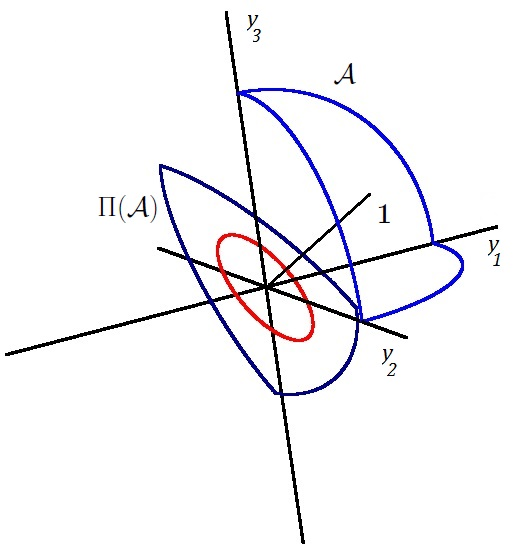
\includegraphics[width=2.75in]{minSS3dSampleSpace.jpg}
\caption{A depiction of $\mathcal{A}$, $\Pi(\mathcal{A})$, and the
  unit circle for the illustrative example where $b_{1}(\mathbf{1},\by)=\min(\by)=0$ and
  $s(\mathbf{1},\by)=\sum (y_i -b_{1}(\mathbf{1},\by))^2 =1$.
$\mathcal{A}$ is the combination of three quarter circles, one
  on each plane defined by $y_i=0$. The projection of this manifold
  onto the deviation space is depicted by the bowed triangular shape
  in the plane defined by $\sum y_i=0$. The circle in this plane
  represents the sample space for the intermediate sample $\bz^*$. Also
  depicted is the vector $\mathbf{1}$, the design matrix for the
  location and scale setting.}
\label{fig:sampSpace}
\end{figure}


%The \green{unit} sphere from
%which the initial sample is taken is depicted as the red circle in this plane.  In general, this is the unit sphere in the $n-p$ dimensional space $\mc{C}^\perp(X)$.  
%With the domain of $h(\dot)$ restricted to the unit sphere in $\mathcal{C}^{\perp}(X)$, the range is still the entirety of $\mathcal{A}$. This is important so that the support of the proposal distribution (i.e. the $h(\dot)$) is at least as large as the support of the target  $f(\by | \theta, y\in \mathcal{A})$, which is  $\mathcal{A}$; a necessary condition for convergence of the Metroplis-Hastings algorithm. To see that the range of $h(\dot)$ is $\mathcal{A}$, consider the any $\by \in \mathcal{A}$ and its projection onto $\mathcal{C}^{\perp}(X)$: $Q\by$ where $Q = I - XX^{\top}$ \footnote{We have used condition \ref{fullRank} to assume  without loss of generality  that the columns of $X$ form an orthonormal basis for $\mc{C}(X)$ (i.e., $X^\top X=I$).}. It is easy to show that $\bz^{*} = Q\by/||Q\by||$ is on the unit sphere and $h(\bz^{*}) = \by$.
%
%
%
%To see this, note that the theorem shows that any $\by$ expressed as in the theorem is an element of $\mc A$. Further, any $\by \in \mc A$ can be expressed as in the theorem by simply replacing $\bz^{*}$ with $\by$. The set $\mathcal{A}$ is an $n - p - 1$ dimensional space:  there are $p$ constraints imposed by the regression coefficients and one further constraint imposed by the scale.  The form of the set is determined by the statistic $T(\cdot)$.  

%As an example, Figure~\ref{fig:sampSpace} provides an artificial low-dimensional visualization of such a set for a location-scale model.  In the figure, $n = 3$, and the conditioning statistic is $T(\by)=(\min(\by), \sum (y_i - \min(\by))^2)$. The set $\mathcal{A}$ is depicted for $T(\by_{obs})=(0,1)$ which we describe as a ``warped triangle'' in light blue, with each side corresponding to a particular coordinate of $\by$ being the minimum
%value of zero. The other two coordinates are restricted by the scale statistic to lie on the quarter circle of radius one in the positive orthant. In general, this set may be compact and given by a closed
%curve, as in the figure, or it may be unbounded, depending on the choice of $T(\by)$.  The other sets labeled in the figure will be described shortly.
%

%Further, this reduced space is chosen so that the range of the map is the entirety of $\mathcal{A}$.  %The Jacobian does not cancel in \eqref{MHRatio}, since the scaling depends on the initial proposal. 

%The reduced space from which the initial sample is taken is simply the
%unit sphere \green{\sout{restricted to} in} the orthogonal complement of the column space of the design matrix (i.e., the least squares residual space). To help understand the density of the proposal derived from the transformation of this initial sample we introduce the following notation. Denote the column space of the design matrix $X$ by $\mathcal{C}(X)$ and its orthogonal complement by $\mc{C}^\perp(X)$. 
%\green{\sout{This} The latter} is the least squares residual space which we will often refer to as the `deviation space'.  The projection of the set $\mathcal{A}$ onto the deviation space is 
%\begin{equation}
%\label{sampleSpacePerp}
%\Pi(\mathcal{A})=\{\bz\in \mathbb{R}^n |\ \exists\ \by\in \mathcal{A}\
%s.t.\ \bz=Q \by \}
%\end{equation} 
%where $Q$ is the projection matrix onto  $\mc{C}^\perp(X)$. Explicitly, $Q=I-H$ with $H=XX^\top$ where we assume, without
%loss of generality following condition \ref{fullRank},  that the
%columns of $X$ form an orthonormal basis for $\mc{C}(X)$
%(i.e., $X^\top X=I$). It will also be helpful at times to write $Q=WW^{\top}$ where the columns of $W$ form an orthonormal basis for $\mc{C}^\perp(X)$. This set has been introduced because we will first transform the initial distribution on the sphere to the distribution on this set. Then we will transform to the \green{\sout{sample space} set} $\mc A$.

%Returning to the artificial example, Figure~\ref{fig:sampSpace}
%depicts $\Pi(\mathcal{A})$ as well as the sphere from which we obtain
%the initial sample. The column vector $X=\bf{1}$ spans $\mc{C}(X)$ and
%is shown as a reference. The triangle with bowed sides in dark
%  blue is  $\Pi(\mathcal{A})$, the projection of $\mc A$ onto the
%plane orthogonal to $\mb 1$ (i.e., $\mc{C}^\perp(X)$). The \green{unit} sphere from
%which the initial sample is taken is depicted as the red circle in this plane.  In general, this is the unit sphere in the $n-p$ dimensional space $\mc{C}^\perp(X)$.  
%
%For the transformation of the initial proposal $\bz^*$ on the surface of the sphere to $\by\in \mc A$ , we first move to a point on $\Pi(\mathcal{A})$ through a 
%simple scaling of $\bz^*$.  This is followed by undoing the projection with a move from 
%$\Pi(\mathcal{A})$ to its (unique) preimage on $\mathcal{A}$. Together, these two steps correspond to the
%transformation in Theorem~\ref{Transformation}.  The introduction of
%the sphere in $\mc {C}^\perp (X)$ as the initial proposal surface
%along with properties \ref{regEq}-\ref{scaleEq2Reg} ensure that the mapping is
%1-1. In particular, property
%\ref{scaleEq2Reg} ensures the scaling to be unique and \ref{regIn}
%implies that the scale statistic is unchanged when undoing the
%projection. Property \ref{regEq} ensures the uniqueness of undoing the
%projection.  The general proposal strategy is summarized as follows:
%\begin{enumerate}
%\item Sample $\bz^*$ from a distribution with known density on the unit sphere in $\mc{C}^\perp(X)$.
%\item Calculate the Jacobian of \green{the} transformation in Theorem \ref{Transformation} in two steps.
%\begin{enumerate}
%\item Scale from unit sphere to $\Pi(\mathcal{A})$: $\bz=\frac{s(X,\boldsymbol{y}_{obs})}{s(X, \boldsymbol{z}^{*})}\bz^{*}$
%\item Shift  from $\Pi(\mathcal{A})$ to $\mathcal{A}$: $\by=\bz+X\left(\bb(X, \by_{obs})-\bb(X, \bz)\right)$
%\end{enumerate}
%\end{enumerate}
%
\subsubsection{Evaluation of the proposal density} 
%Calculation of the appropriate Jacobian of the transformation is absolutely vital and also non-trivial. Writing the transformation from the unit sphere in deviation space to $\mathcal{A}$ in 
%two steps facilitates calculation of the Jacobian in two steps as written above. % \textcolor{blue}{added the following sentence, hopefully it helps}
We now explain each step in computing the Jacobian described above.
%the scale transformation from the unit sphere to $\Pi(\mathcal{A})$, {keeping in mind that the Jacobian of a transformation is simply the ratio of infinitesimal volumes along the tangents of the domain and range of the transformation. 
\vskip 0.05 in
\noindent
{\bf Scale from $\mathbb{S}$ to $\Pi(\mathcal{A})$} \\
The first step is constrained to $\mc{C}^\perp(X)$  and scales the initial $\bz^{*}$ to $\bz=\frac{s(X,\boldsymbol{y}_{obs})}{s(X, \boldsymbol{z}^{*})}\bz^{*}$. For the Jacobian, we consider two substeps: first, the distribution on  $\mathbb{S}$ is transformed to that along a sphere of radius $r=\|\bz\|={s(X,\boldsymbol{y}_{obs})}/{s(X, \boldsymbol{z}^{*})}$. By comparison of the volumes of these spheres, this transformation contributes a factor of $r^{-(n-p-1)}$ to the Jacobian. For the second substep, the sphere of radius $r$ is deformed onto $\Pi(\mathcal{A})$.  This deformation contributes an attenuation to the Jacobian equal to the ratio of infinitesimal volumes in the tangent spaces of the sphere and $\Pi(\mathcal{A})$ at $\bz$.  
Restricting to $\mc{C}^\perp(X)$, this ratio is the cosine of the angle between the normal 
vectors of the two sets at $\bz$.  The normal to the sphere is its radius vector $\bz$. The normal to
$\Pi(\mathcal{A})$ is given in the following lemma.  
\begin{lemma}
\label{gradSTheoremReg}
Assume that conditions \ref{fullRank}-\ref{supReal}, \ref{as}, and \ref{regIn} hold and $\by\in \mathcal{A}$. Let 
$\nabla s(X,\by)$ denote the
gradient of the scale statistic with respect to the data vector evaluated at
$\by$.  Then $\nabla s(X,\by)\in \mc{C}^\perp(X)$ and is 
normal to $\Pi(\mathcal{A})$ at $\bz=Q\by$  in $\mc{C}^\perp(X)$.
\end{lemma}
As a result of the lemma, the contribution to the  Jacobian of this attenuation is 
\begin{equation}
\label{cosine}
\cos(\gamma)=\frac{\nabla s(X,\by)^\top \bz}{\|\nabla
s(X,\by)\| \|\bz\|},
\end{equation}
where $\gamma$ is the angle between the two normal vectors.
This step is visualized in Figure~\ref{fig:stretchDeform} for the artificial
location-scale example.  The figure pictures only the $\mathcal{C}^{\perp}(X)$,
which in this case is a plane. The unit sphere (here, the
solid circle) is stretched to the dashed sphere contributing
$r^{-(n-p-1)}$ to the Jacobian as seen in panel (a). In panel (b), the
dashed circle is transformed onto $\Pi(\mc A)$ contributing
$\cos(\gamma)$ to the Jacobian. The normal vectors in panel (b) are
orthogonal to the tangent vectors of $\Pi(\mc A)$ and the circle. %As stated above, the Jacobian is the ratio of infinitesimal lengths along these tangent vectors. This is the same as the ratio of the infinitesimal lengths of the normal vectors (i.e., $\cos(\gamma)$). This generalization extends to higher dimensions where the `lengths' along the tangent vectors become volumes along the tangent spaces. 

%\begin{sidewaysfigure}[t]
%\centering
%\captionsetup{justification=centering}
%\subcaptionbox{}{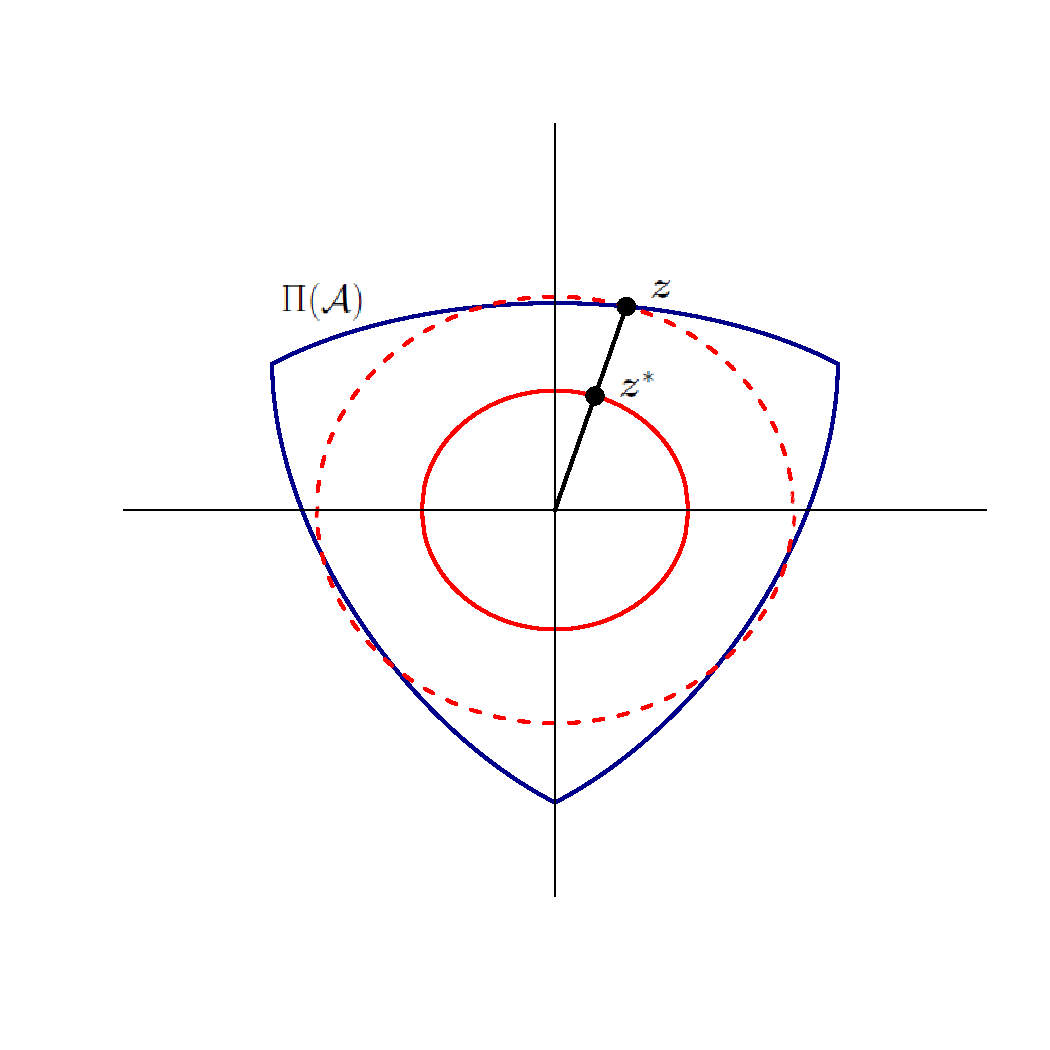
\includegraphics[width=4in]{minSSZSpace3.pdf}}\quad
%\subcaptionbox{}{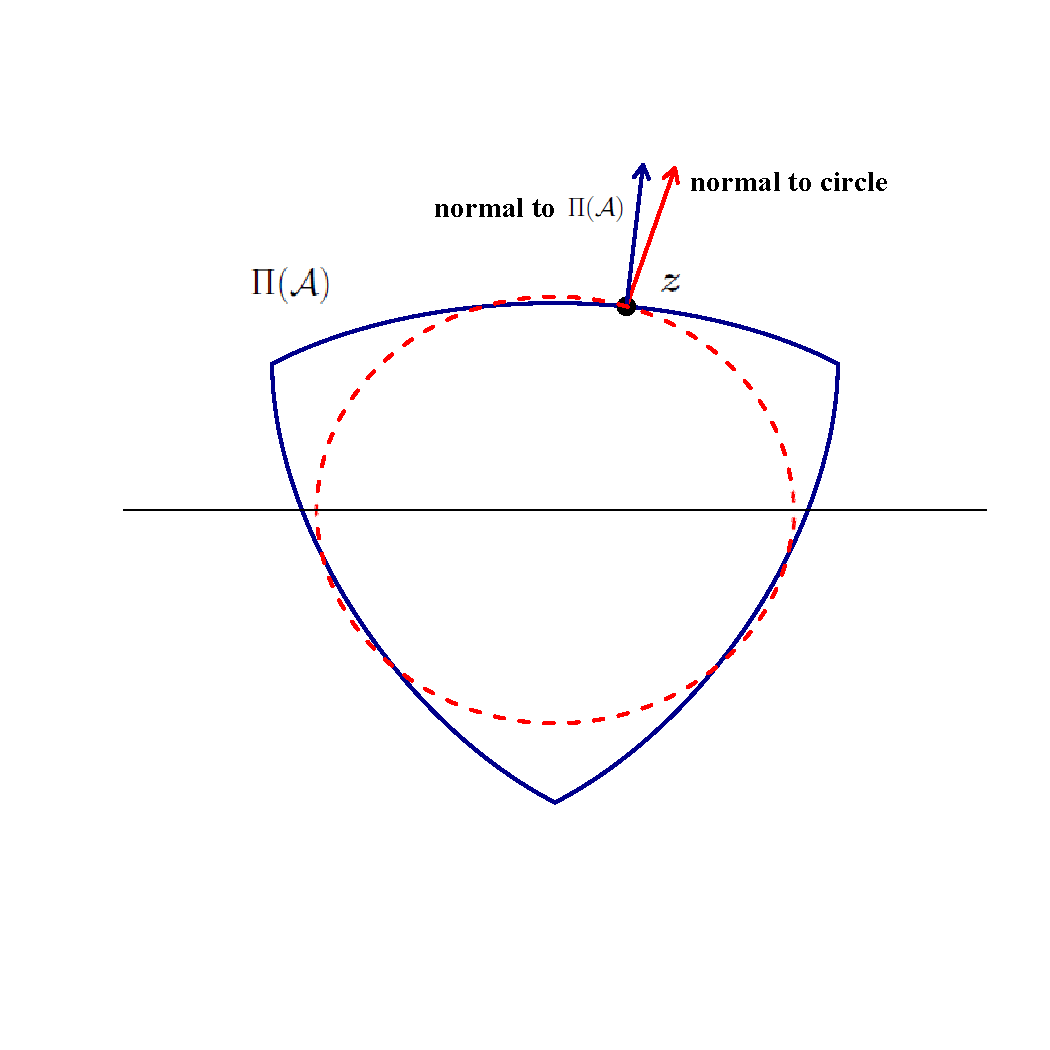
\includegraphics[width=4in]{minSSZSpace5.pdf}}
%\caption{Panel (a) contains a depiction of the stretch from $\bz^{*}$
%  to $\bz$. The adjustment for the stretch transforms the density
%  along the unit circle to the density along the circle of radius
%  $\|\bz\|$ (dashed circle).  Panel (b) contains a depiction of the
%  deformation from the distribution along the circle to the
%  distribution along $\Pi(\mathcal{A})$. The adjustment can be seen to
%  be the cosine of the angle between the normals to each manifold.}
%\label{fig:stretchDeform}
%\end{sidewaysfigure}

\begin{figure}[t]
\centering
{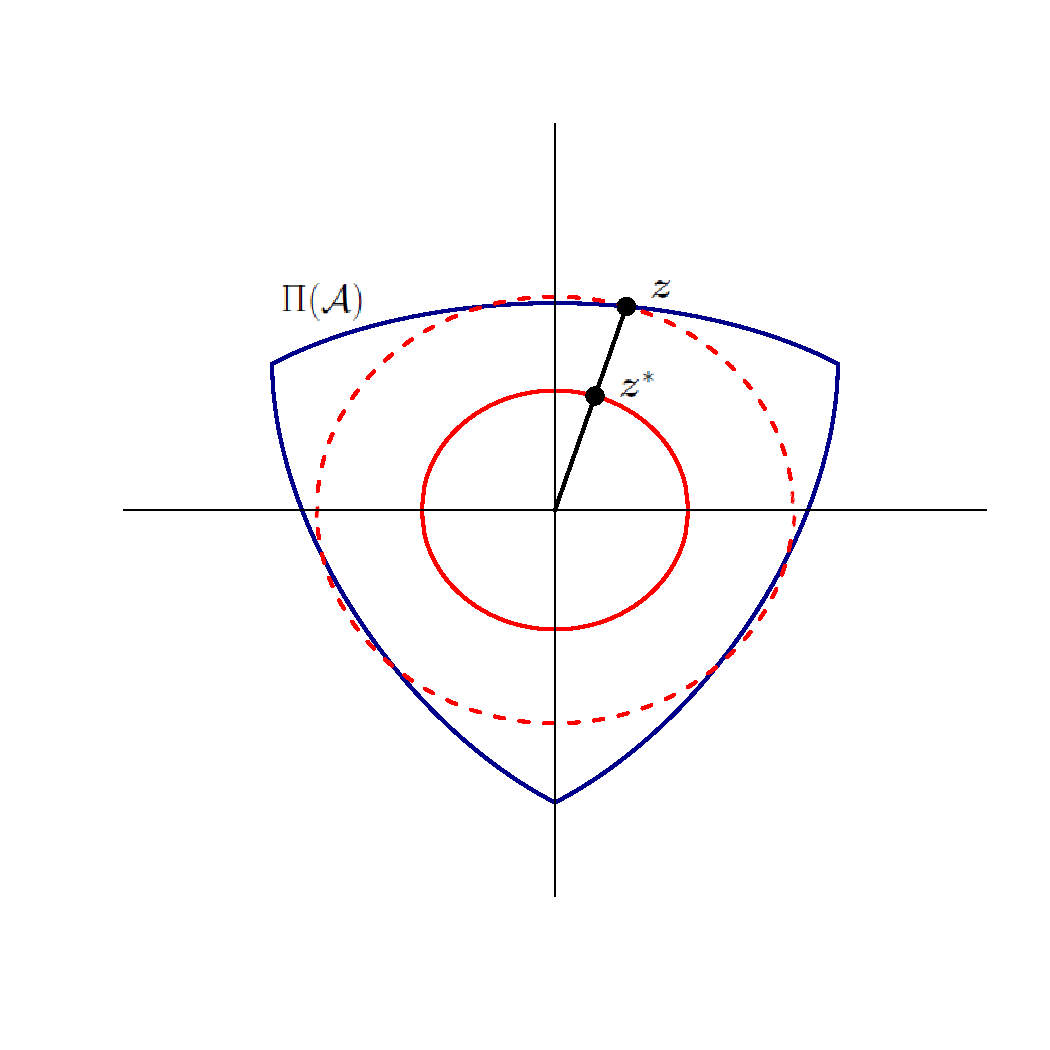
\includegraphics[width=2.9in]{minSSZSpace3.pdf}}
{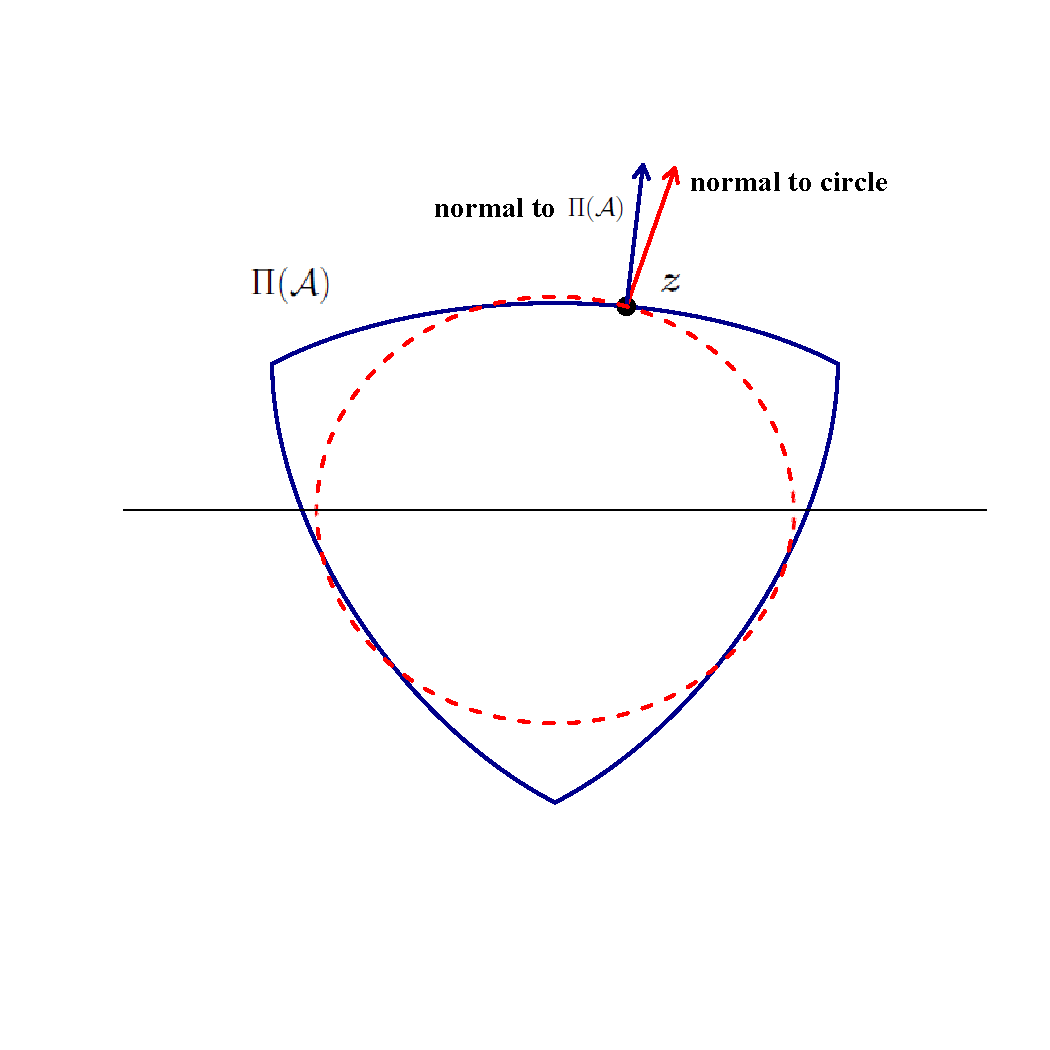
\includegraphics[width=2.9in]{minSSZSpace5.pdf}}
\label{fig:stretchDeform}
\caption{sdasfda}
\end{figure}

%\begin{figure}[t]
%\centering
%{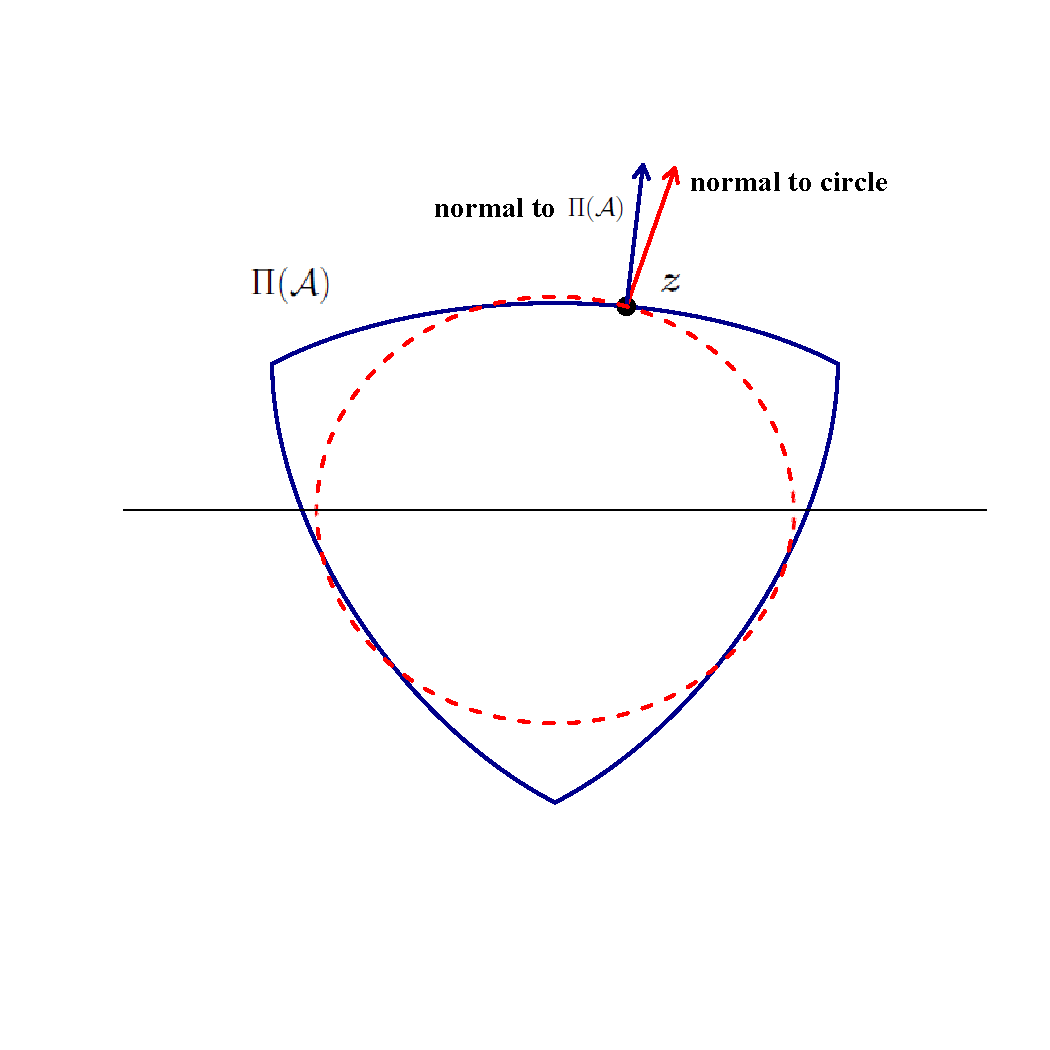
\includegraphics[width=2in]{minSSZSpace5.pdf}}
%\label{fig:stretchDeform}
%\caption{sdassfsadfda}
%\end{figure}
%%
%\subcaptionbox{}{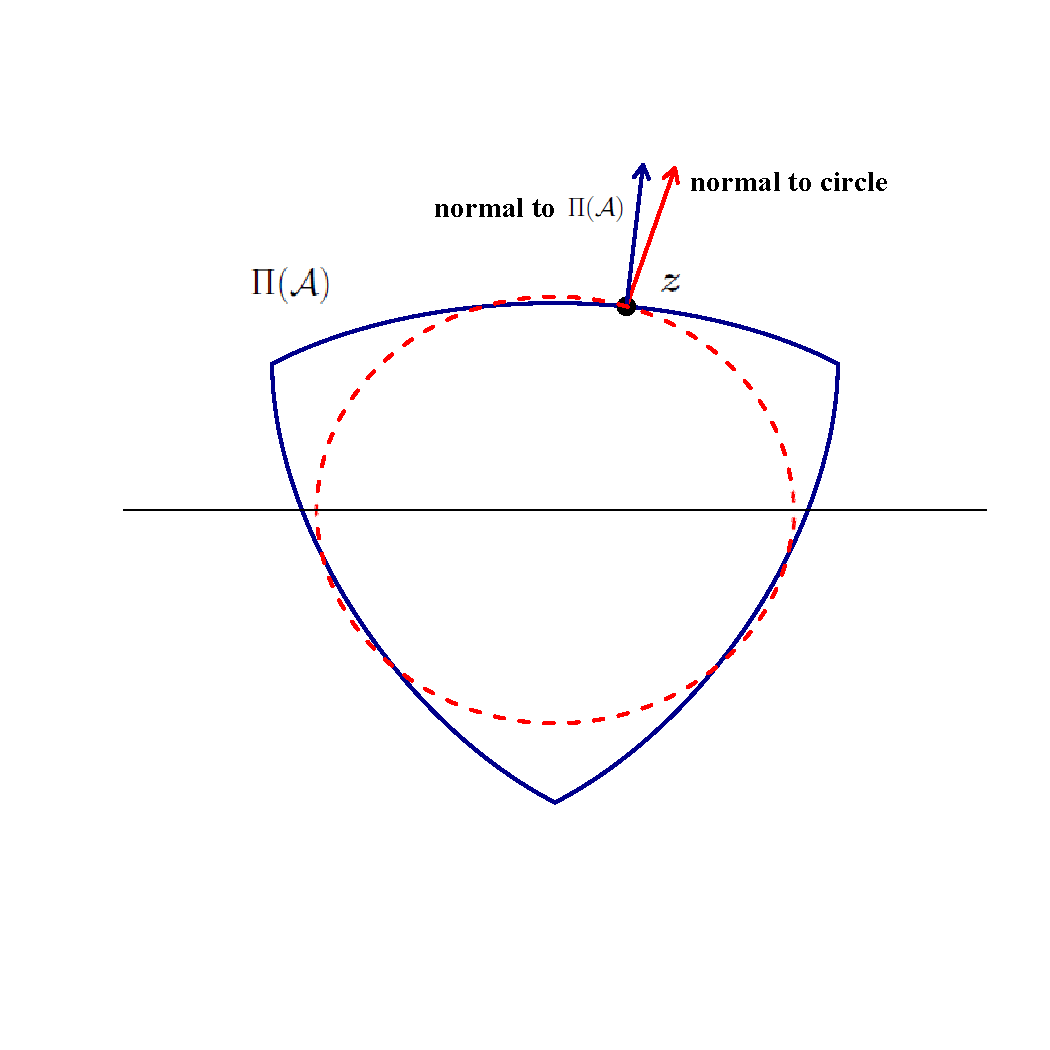
\includegraphics[width=4in]{minSSZSpace5.pdf}}
%\caption{Panel (a) contains a depiction of the stretch from $\bz^{*}$
%  to $\bz$. The adjustment for the stretch transforms the density
%  along the unit circle to the density along the circle of radius
%  $\|\bz\|$ (dashed circle).  Panel (b) contains a depiction of the
%  deformation from the distribution along the circle to the
%  distribution along $\Pi(\mathcal{A})$. The adjustment can be seen to
%  be the cosine of the angle between the normals to each manifold.}
%\label{fig:stretchDeform}
%\end{sidewaysfigure}



\vskip 0.05 in
\noindent
{\bf Shift from $\Pi(\mathcal{A})$ to $\mathcal{A}$} \\
The final piece of the Jacobian comes from the transformation from
$\Pi(\mathcal{A})$ to $\mathcal{A}$.  %For this we return to the full $n$ dimensional space.  
This step involves a shift of
$\bz$ to $\by$ along the column space of $X$. Since the shift depends on 
$\bz$, the density on the set 
$\Pi(\mathcal{A})$ is deformed by the shift. The
contribution of this deformation to the Jacobian is, again,
the ratio of the infinitesimal volumes along $\Pi(\mathcal{A})$ at $\bz$ to the
corresponding volume along $\mathcal{A}$ at $\by$. 
The ratio is calculated by considering the volume of the
projection of a unit hypercube in the tangent space of $\mathcal{A}$
at $\by$ onto $\mc{C}^\perp(X)$.
Computational details are
given in the following lemmas and subsequent theorem. Throughout, let
$\mc T_{y}(\mc A)$ and $\mc T_{y}^{\perp}(\mc A)$ denote the tangent
space to $\mc A$ at $\by$ and its orthogonal complement respectively. All gradients denote with $\nabla$ are with respect to the data vector.
\begin{lemma}
\label{lem:basis}
Assume that conditions \ref{fullRank}-\ref{regEq} and \ref{regIn}-\ref{scaleEq2Reg} hold.  Then the $p+1$ gradient vectors 
$\nabla s(X,\by), \nabla b_1(X,\by),\dots, \nabla b_p(X,\by)$ form a
basis for $\mc T_{y}^\perp(\mc A)$ with probability one.
\end{lemma}

The lemma describes construction of a basis for $\mc T_{y}^\perp(\mc A)$, leading to a 
basis for $\mc T_{y}(\mc A)$.  Both of these bases can be orthonormalized.  
Let $A=[a_{1},\dots,a_{n-p-1}]$  and $B=[b_1,\dots,b_{p+1}]$ denote the 
matrices whose columns contain the orthonormal bases for  $\mc T_{y}(\mc A)$ and  $\mc T^{\perp}_{y}(\mc A)$, respectively.  
The columns in $A$ define a unit hypercube in $\mc T_{y}(\mc
  A)$ and their projections onto $\mc{C}^\perp(X)$ define a parallelepiped.
We defer construction of $A$ until later. 

\begin{lemma}
\label{lem:fullrank}
Assume that conditions \ref{fullRank}-\ref{regEq} and \ref{regIn}-\ref{scaleEq2Reg} hold.  
Then the $n\times (n-p-1)$ dimensional matrix $P=QA$ is of full column rank.
\end{lemma}

As a consequence of this lemma, 
the parallelepiped spanned by the columns of $P$ is not
degenerate (it is $n-p-1$ dimensional), and its volume
is given by
\begin{equation}
\label{eq:volume}
\text{Vol} (P) := \sqrt{\text{det}(P^\top P)}=\prod_{i=1}^{r} \sigma_i
\end{equation}
where $r=\text{rank} (P)=n-p-1$ and $\sigma_1\geq
\sigma_2\geq\dots\geq\sigma_r>0$ are the singular values of $P$ (e.g.,
\cite{miao1992}). 
Combining Lemmas \ref{lem:basis} and \ref{lem:fullrank} above leaves us with the following result concerning the calculation of the desired Jacobian.  
\begin{theorem}
\label{Jacobian}
Assume that conditions \ref{fullRank}-\ref{regEq} and \ref{regIn}-\ref{scaleEq2Reg} hold.  Then the
Jacobian of the transformation from the distribution along 
$\Pi(\mc A)$ to that along $\mc A $ is equal to the volume given in \eqref{eq:volume}.
\end{theorem}

\vskip 0.05 in
\noindent
{\bf The proposal density} \\
Putting all the pieces of the Jacobian together we have the following result. Any dependence on other variables, including current states in the Markov chain, is made implicit. 
\begin{theorem} 
Assume that conditions \ref{fullRank}-\ref{scaleEq2Reg} hold.  Let $\bz^{*}$ be sampled on the unit sphere in $\mc {C}^\perp (X)$ with density $p(\bz^{*})$.  Using the transformation of $\bz^*$ to $\by\in \mc A$ described in Theorem \ref{Transformation}, the density of $\by$ is
\begin{equation}
\label{dens:ystst}
p(\by)=p(\bz^*) r^{-(n-p-1)} \cos(\gamma)\text{Vol} (P)
\end{equation}
where $r={s(X,\boldsymbol{y}_{obs})}/{s(X,  \boldsymbol{z}^{*})}$,
and $\cos(\gamma)$ and $\text{Vol} (P)$ are as in equations \eqref{cosine} and \eqref{eq:volume}, respectively. 
\end{theorem} 

%In practice, computing $A$ directly to find $P$ and $\text{Vol} (P)$ is computationally intensive as it involves orthogonalization of $n$ vectors in $n$-dimensional space. 
A few details for computingthe needed quantities are worth further explanation. Computing $\text{Vol} (P)$ involves finding an orthornormal matrix $A$ whose columns span $\mc T_{y}(\mc A)$. This matrix can be found by supplementing $B$ with a set of $n$ linearly independent columns on the right, and apply Gram-Schmidt orthonormalization.  This is $\mc O(n^3)$ and is infeasibly slow when $n$ is large because it must be repeated at each iterate of the MCMC when a complete data set is drawn.  However, using results related to \textit{principal angles} found in \cite{miao1992} the volume \eqref{eq:volume} can be computed using only $B$. $B$ is constructed by Gram-Schmidt orthogonalization of $\nabla s(X,\by), \nabla b_1(X,\by),\dots, \nabla b_p(X,\by)$, which is  $\mc O(np^2)$;  a 
considerable reduction in computational burden when $n \gg p$. 
%Further, the singular values of $P=QA$ are also the singular values of
%$W^\top A$ where $Q=WW^{\top}$, which can be easily obtained through $B$.
The following corollary formally states how computation of $A$ can be circumvented. 
\begin{corollary}
\label{theorem:sings}
Let $U$ be a matrix whose columns form an orthonormal basis for $\mc C (X)$ and set $Q=WW^{\top}$ where the columns of $W$ form an orthonormal basis for $\mc{C}^\perp(X)$. Then the non-unit singular values of $U^\top B$ are the same as the non-unit singular values of $W^\top A$.
\end{corollary} 
\noindent The lemma implies the $\text{Vol} (P)$ is the product of the singular values of $U^\top B$. 

Second, the gradients of $\nabla s(X,\by), \nabla b_1(X,\by),\dots, \nabla b_p(X,\by)$ are easily computed. For example, below we consider M-estimators defined by the estimating equations:
\begin{eqnarray}
\label{Mest}
 \sum_{i=1}^n \psi\left(\frac{y_i - x_{i}^{\top}\bb(\by,X)}{s(\by,X)}\right)= & 0 \\
 \sum_{i=1}^n \chi\left(\frac{y_i - x_{i}^{\top}\bb(\by,X)}{s(\by,X)}\right)= & 0, \nonumber 
\end{eqnarray} 
where $\psi$ and $\chi$ are almost surely differentiable. Differentiating this system of equations with respect to each $y_{i}$ can be used to find the gradients. In theory, finite differences could also be used. 



%%%%%%%%%%%%%%%%%%%%%%%%%%%%%%%%%%%%%%%%%%%%%%%%%%%%%%%%%%%%
%
% Applications
%
%%%%%%%%%%%%%%%%%%%%%%%%%%%%%%%%%%%%%%%%%%%%%%%%%%%%%%%%%%%%
%\section{Applications}
%In this section we apply the restricted likelihood to both simulated and real data. 

\section{Simulated Data}
\label{simData}
We study the performance of the restricted likelihood in a hierarchical setting contaminated with outliers. Specifically, simulated data come from the following data generating model:
\begin{align}
\label{gensim2}
\begin{split}
& \theta_{i}  \sim   N(\mu, \tau^{2}),  \ i = 1, 2, \dots, 90  \\ 
& y_{ij} \sim (1-p_{i})N(\theta_{i}, \sigma^{2}) + p_{i}N(\theta_{i}, m_{i}\sigma^{2}),\  j = 1, 2,..., n_{i}
\end{split}
\end{align}
with $\mu = 0, \tau^{2} = 1, \sigma^{2} = 4$. The values of $p_{i}, m_{i}$, and $n_{i}$ depend on the group and are formed using 5 replicates of the full factorial design over factors $p_{i},m_{i},n_{i}$ with levels $p_{i} = .1, .2, .3$, $m_{i} = 9, 25$, and $n_{i} = 25, 50, 100$. This results in 90 groups that have varying levels of outlier contamination and sample size. We wish to build models that offer good prediction for the good portion of data within each group. The full model for fitting is a corresponding normal model without contamination:
\begin{equation}
\label{fullsim2}
\begin{split}
& \mu \propto 1, \  \tau^{2} \propto \tau^{-2}, \\
& \theta_{i}\sim N(\mu, \tau^{2}), \  \sigma^{2}_{i} \sim IG(a_{s}, b_{s}),  \ i = 1, 2, \dots, 90, \\ 
& y_{ij}\sim  N(\theta_{i},\sigma^{2}_{i}), \ j = 1, 2, \dots, n_{i}.
\end{split}
\end{equation}
For the restricted likelihood versions we condition on robust M-estimators of location and scale in each group: $T_{i}(y_{i1}, \dots, y_{in_{i}}) = (\hat\theta_{i}, \hat\sigma^{2}_{i}), i = 1, 2, ..., 90$.  These estimators are solutions to equation \eqref{Mest} (where $x_{i}\equiv 1$) with user specified $\psi$ and $\chi$ functions designed to discount outliers. The two versions use Huber's and Tukey's $\psi$ function, while both versions use Huber's $\chi$ function. The tuning parameters associate with these functions are chosen so that the estimators are $95\%$ efficient under normally distributed data. Both of these are well known M-estimators used in robust regression settings  \citep{huber2009}.  %We will see that his choice has some interesting effects on the results. %These estimators are implemented in the R function \texttt{MASS::rlm} with \cite{huber2009} providing further details. 

To complete the specification of model \eqref{fullsim2},  $a_{s}$ and $b_{s}$ are fixed to a variety of values representing different levels of prior knowledge. For each we set $b_{s} = 4a_{s}c$ resulting in a prior mean for each $\sigma^{2}_{i}$ of $\frac{4ca_{s}}{a_{s}-1}, \ a_{s} >1$. The precision is $\frac{(a_{s} -1)^{2}(a_{s}-2)}{(4ca_{s})^{2}}$; meaning the larger $a_{s}$, the more informative the prior. With $c = 1$ the shrinkage (for large $a_{s}$) is to the true value of $\sigma^{2} = 4$. We consider $a_{s} = 1.25,  5, 10$ and $c = 0.5, 1, 2$. %Values of $c \neq 1$ will result in shrinkage towards the wrong value of $\sigma^{2}$.

$K = 30$ data sets are generated from \eqref{gensim2}. For each data set and each pair $(a_{s}, c)$, the Bayesian models are fit using MCMC. The MCMC for the restricted likelihood version requires no further computational details other than those described for the traditional Bayesian model in Section \ref{BayesLinMod}. This is because there are conditioning statistics for each group and the model's conditional independence between the groups allows the data augmentation described earlier to be performed independently within each group. That is, there is a separate Gibbs step for each group  generating group level data matching the statistics for that group. 

To assess the predictive capability, the models are compared using Kullback-Leibler (KL) divergence from the distribution of good data to the posterior predictive distribution. Specifically, for the $i^{th}$ group of the $k^{th}$ simulated data set $\by_{k}$ compute:
\begin{equation}
\label{kl}
KL^{(M)}_{ik} = \int \log \frac{f(\tilde y | \theta_{i}, \sigma^{2})}{f_{i}(\tilde y | M, \by_{k})}  f(\tilde y | \theta_{i}, \sigma^{2}) \ dy
\end{equation}
where $M$ indexes the fitting model, $f(\tilde y | \theta_{i}, \sigma^{2}) = N(\tilde y | \theta_{i}, \sigma^{2})$; the mean $\theta_{i}$, variance $\sigma^{2}$ normal pdf evaluated at $\tilde y$. For the Bayesian models ${f_{i}(\tilde y | M, \by_{k})} = \int f(\tilde y |\theta_{i}, \sigma_{i}^{2}) \pi(\theta_{i}, \sigma^{2}_{i} | M, \by_{k})d\theta_{i}d\sigma^{2}_{i}$ where $\pi(\theta_{i}, \sigma^{2}_{i} | M, \by_{k})$ is the posterior for the $i^{th}$ group model parameters under model $M$ for the $k^{th}$ data set. $M$ denotes either the full normal theory model \eqref{fullsim2} or one of the two restricted likelihood versions, along with $a_{s}$ and $c$. For the classical robust fits, we set $f_{i}(\tilde y | M, \by_{k}) = N(\tilde y|\hat\theta_{i}, \hat\sigma^{2}_{i})$ as a groupwise plug-in estimator for the predictive distribution. The classical fits are done separately for each group with no consideration of the hierarchical structure between the groups. The overall mean $\overline{KL}^{(M)}_{{\cdot}{\cdot}} = \frac{1}{90K} \sum_{k = 1}^{K} \sum_{i=1}^{90} KL^{(M)}_{ik}$ is used to compare the models where smaller means correspond to better fits. Sampling variation is summarized with the standard error $SE(\overline{KL}^{(M)}_{{\cdot} k}) = \sqrt{\frac{1}{K(K-1)}\sum_{k = 1}^{K} (\overline{KL}^{(M)}_{{\cdot} k} - \overline{KL}^{(M)}_{{\cdot}{\cdot}})^{2}}$ where $\overline{KL}^{(M)}_{{\cdot} k} = \frac{1}{90}\sum_{i = 1}^{90} KL^{(M)}_{ik}$.
 
Figure \ref{kl_sim} displays $\overline{KL}^{(M)}_{{\cdot}{\cdot}}$  with error-bars plus/minus one $SE(\overline{KL}^{(M)}_{{\cdot} k})$ for each $a_{s} = 1.25,  5, 10$ and $c = 0.5, 1, 2$. %The panels are for $c = 0.5, 1, 2$ with $a_{s} = 1.25,  5, 10$ on the abscissa. 
The values of $a_{s}$ and $c$, do not effect the classical robust linear models. The normal theory model results are left out as they perform significant worse. Overall, the results are strikingly in favor of the restricted likelihood methods for the range of hyper-parameter values studied. Undoubtably, the most precise and accurate prior studied is  $c = 1$ and $a_{s} = 10$  and this results in the lowest (and best) average KL for both the Tukey and Huber restricted likelihood versions ((shown in the middle panel). $c = 0.5$ performs the worst, but still better than the classical fits. There is evidence that performance starts to degrade as $a_{s} = 10$ as reflected in a larger average KL for $a_{s} = 10$. Here, the prior mean and precision are $2.22$ and $1.62$ and we suspect this is starting to put too much mass on $\sigma^{2}_{i}$ values much smaller than $\sigma^{2}=4$. For $c = 2$, the performance still improves from $a_{s} = 5$ to $a_{s} = 10$. Here the mean is $8.89$ and precision is only $0.1$; apparently not yet large enough to degrade the performance due to an incorrect mean. Lastly, Tukey's statistic performs marginally better than Huber's. This is likely due to the fact that Tukey's estimator trims extreme outliers completely in the estimation procedure \citep{huber2009}.
 
\begin{figure}[t]
\centering
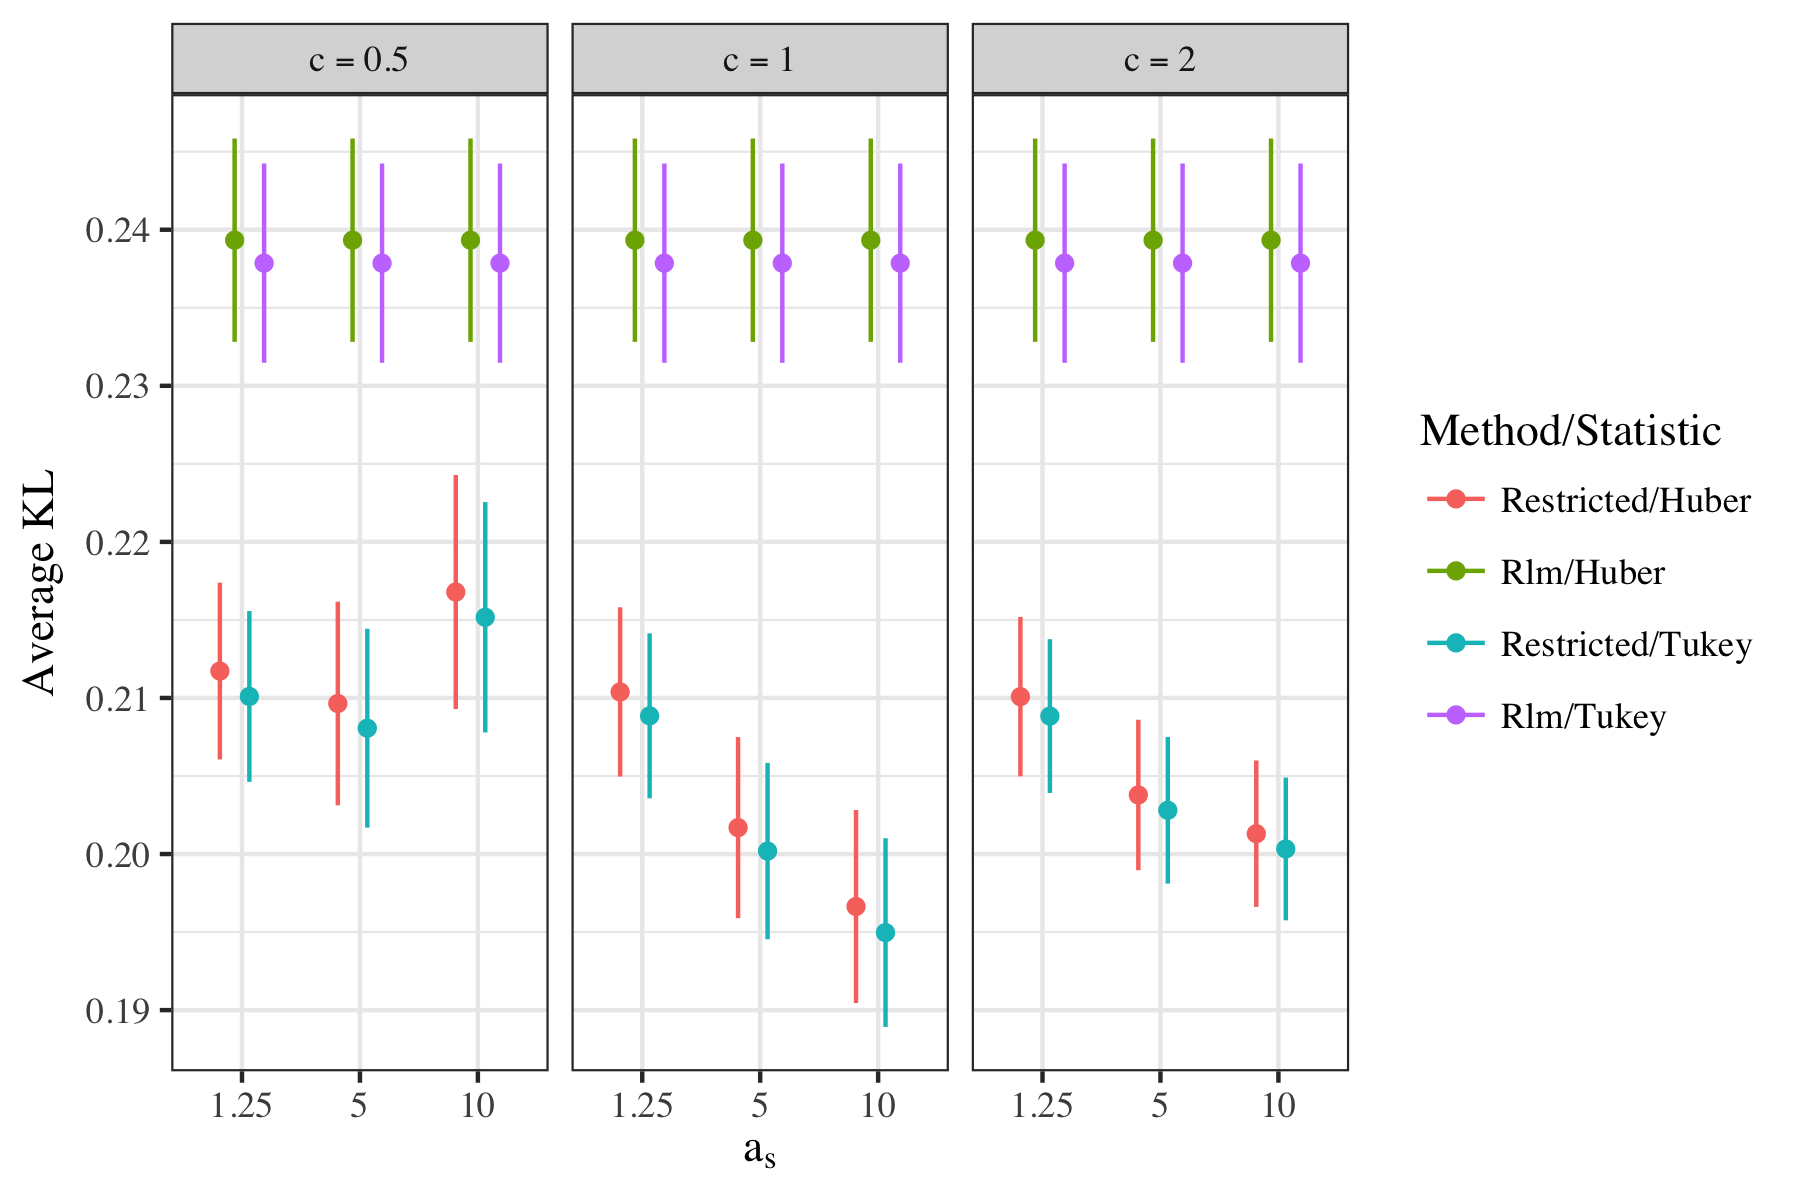
\includegraphics[width = 4in]{kl_sim2_facet_scale.png}
\label{kl_sim}
\caption{Average KL - divergence plus/minus one standard error for each value of $a_{s}$ and $c$. The panels correspond to $c = 0.5$ (left), $c=1$ (middle), and $c=2$ (right) with the values of $a_{s}$ on the horizontal axis.}
\end{figure}

It is also interesting to consider the effects of factors $n_{i}$, $p_{i}$, and $m_{i}$. For a given factor and simulation, the $KL^{(M)}_{ik}$  are averaged by factor level. For the Bayesian models, the averages are also taken over the different values of $a_{s}$ and $c$. Figure \ref{kl_mnp} displays these averages for $m,n,$ and $p$ with error bars plus/minus one standard error. The restricted likelihood versions consistently perform better than their classical counterparts. Intuitively, as the amount of contamination ($p$) increases performance degrades as it becomes more difficult to identify the good data. Likewise, as $n$ increases, the performance for the Bayesian methods become closer to that of the their classical counterparts reflecting the diminishing effect of the prior. However, the decrease of KL-diveregence with $m$ and increase with $n$ is somewhat surprising. To investigate, Figure \ref{boxTheta} and \ref{boxSigma} display boxplots of $(\theta_{i} - \hat\theta_{i})$ and $\hat\sigma_{i}$ for each simulated data set. The $\hat\theta_{i}$'s have no systematic bias however the $\hat\sigma_{i}$'s do; consistently biased upward from the value of $\sigma = 2$ for the good portion of data. As $n$ increases, the bias remains the same and the variation in the estimates gets smaller. Thus, the estimates are getting more certain about an incorrect value; explaining the degradation of the KL - divergence. As $m$ increases, the variance in the estimates gets larger and there is a marginal increase in the bias. Thus, for $m=9$ there is more certainty about an incorrect value and  the increased uncertainty at $m=25$ helps to improve the KL-divergence. %Finally, as $p$ grows the bias of the estimates gets significantly larger; resulting in poorer estimation and poorer KL-divergences.
 
\begin{figure}[t]
\centering
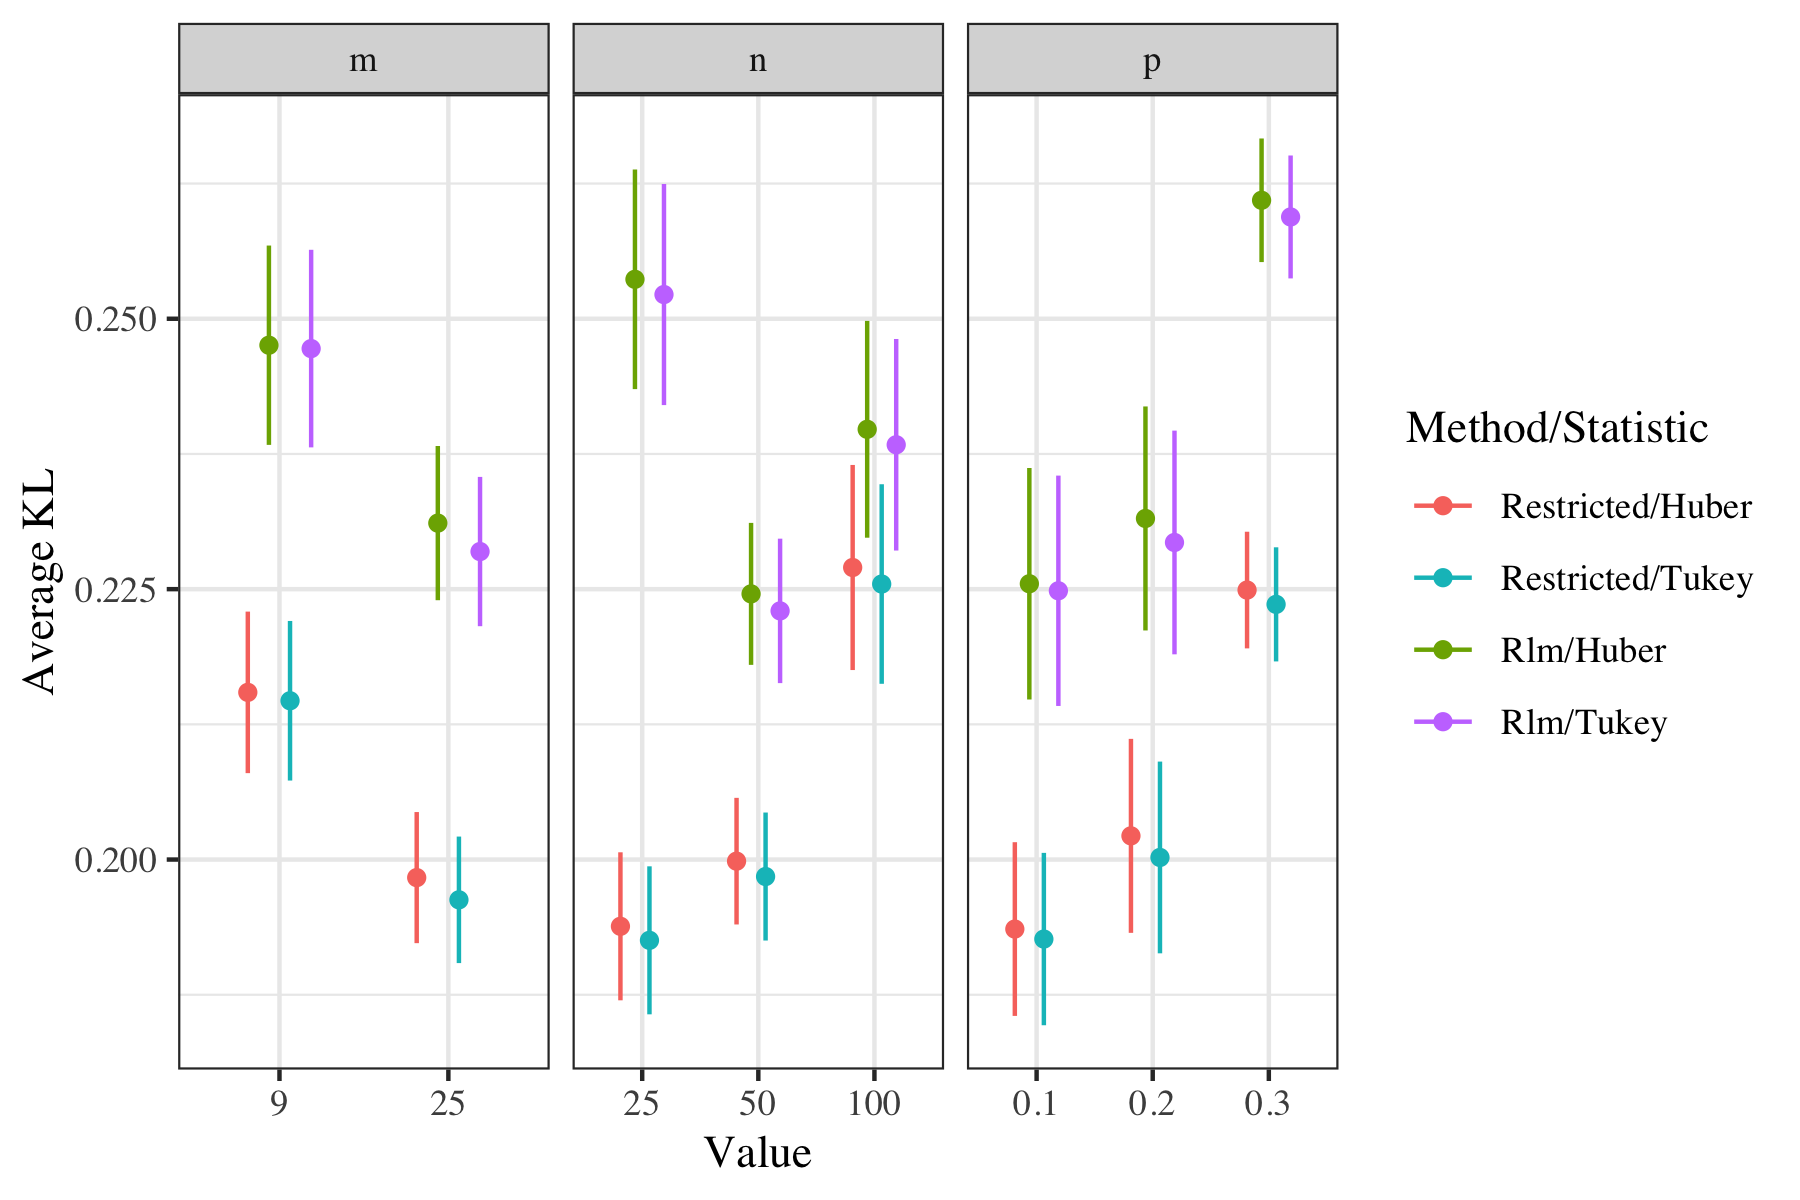
\includegraphics[width = 4in]{kl_sim2_mnp.png}
\caption{Average KL - divergence plus/minus one standard error grouped by the factors $m$ (left), $n$ (middle), and $p$ (right)}
\label{kl_mnp}
\end{figure}
\begin{figure}[t]
\centering
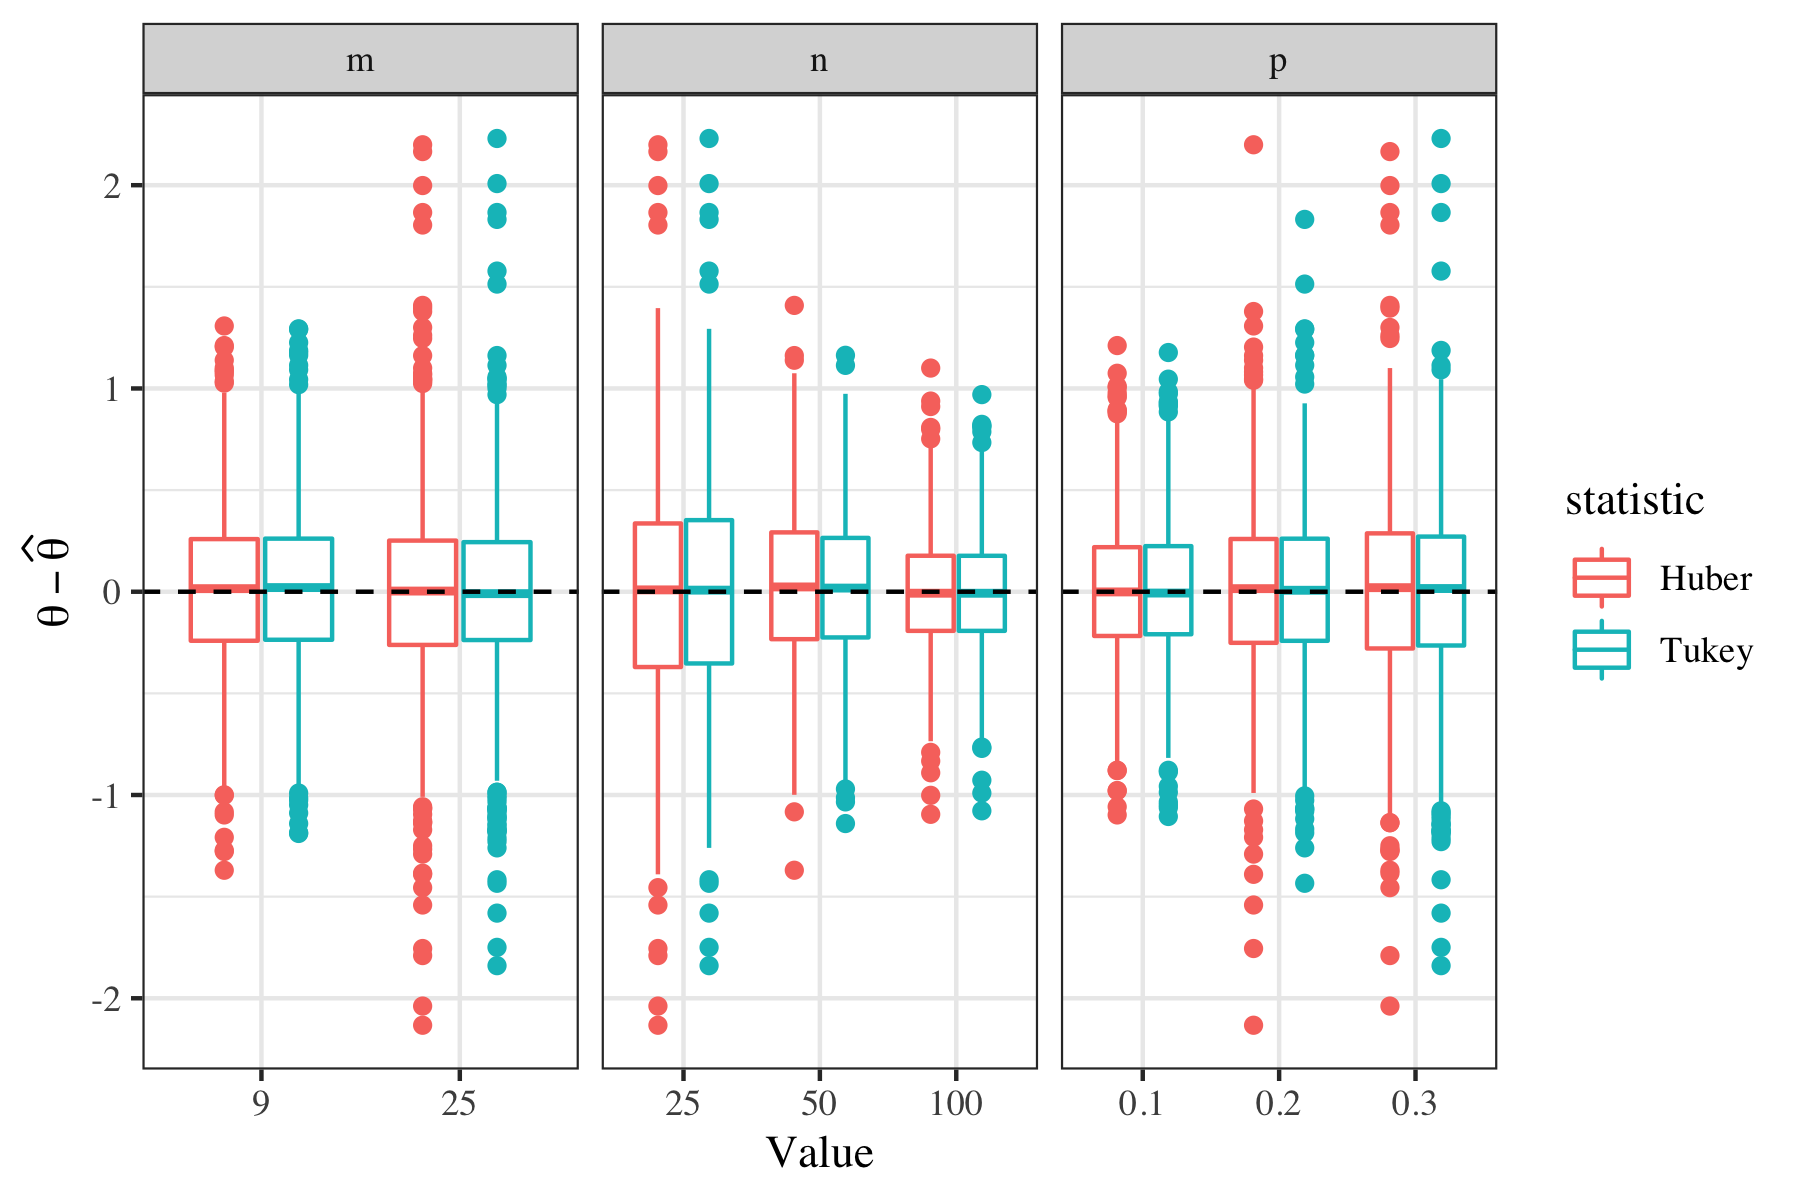
\includegraphics[width = 4in]{rlm_mnp_theta.png}
\caption{Boxplots $(\theta_{i} - \hat\theta_{i})$ across all simulations separated by the values for $m$ (left), $n$ (middle), $p$ (right) where $\hat\theta_{i}$ are the classical robust estimators (Huber's and Tukey's).}
\label{boxTheta}
\end{figure}
\begin{figure}[t]
\centering
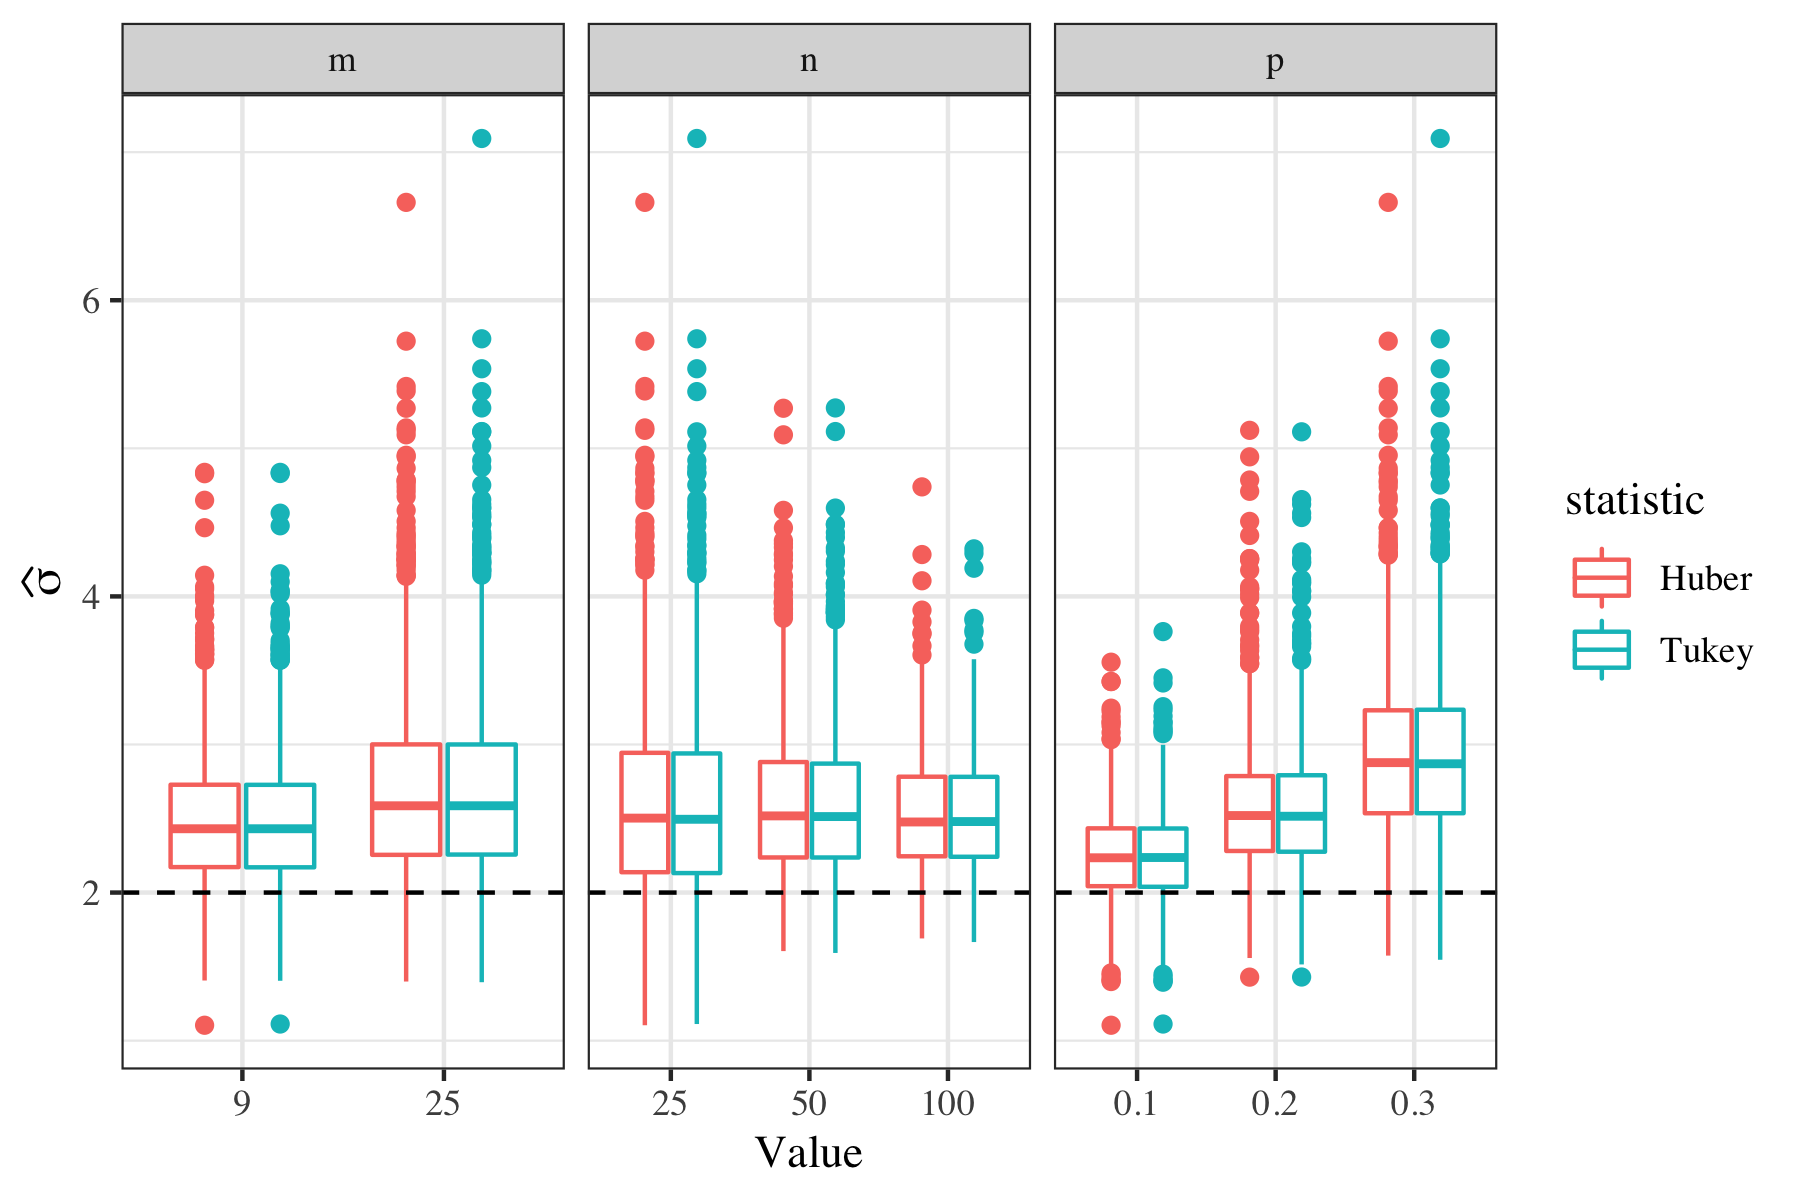
\includegraphics[width = 4in]{rlm_mnp_sigma.png}
\caption{Boxplots of the classical robust estimators (Huber's and Tukey's) for $\sigma_{i}$ across all simulations separated by the values for $m$ (left), $n$ (middle), $p$ (right). The horizontal line at $\sigma = 2$ highlights the true standard deviation of the `good' data.}
\label{boxSigma}
\end{figure}

This simulation shows the potential of the restricted likelihood while highlighting some interesting observations. Specifically, the choice of summary statistics, along with corresponding tuning parameters is important. For the tuning parameters, the standard choice of $95\%$ efficiency at the normal was used.  Under the data generating model here, this choice results in bias in the scale estimation which affects the performance of the method. These choices must be made in both the classical and Bayesian settings. The Bayesian setting allows for the incorporation of informative prior information which, as shown in this example, can dramatically improve prediction. The results are sensitive to the prior, but here we have observed good relative improvement over the classical counterparts for a range of prior choices.   

%
%\begin{figure}[H]
%\centering
%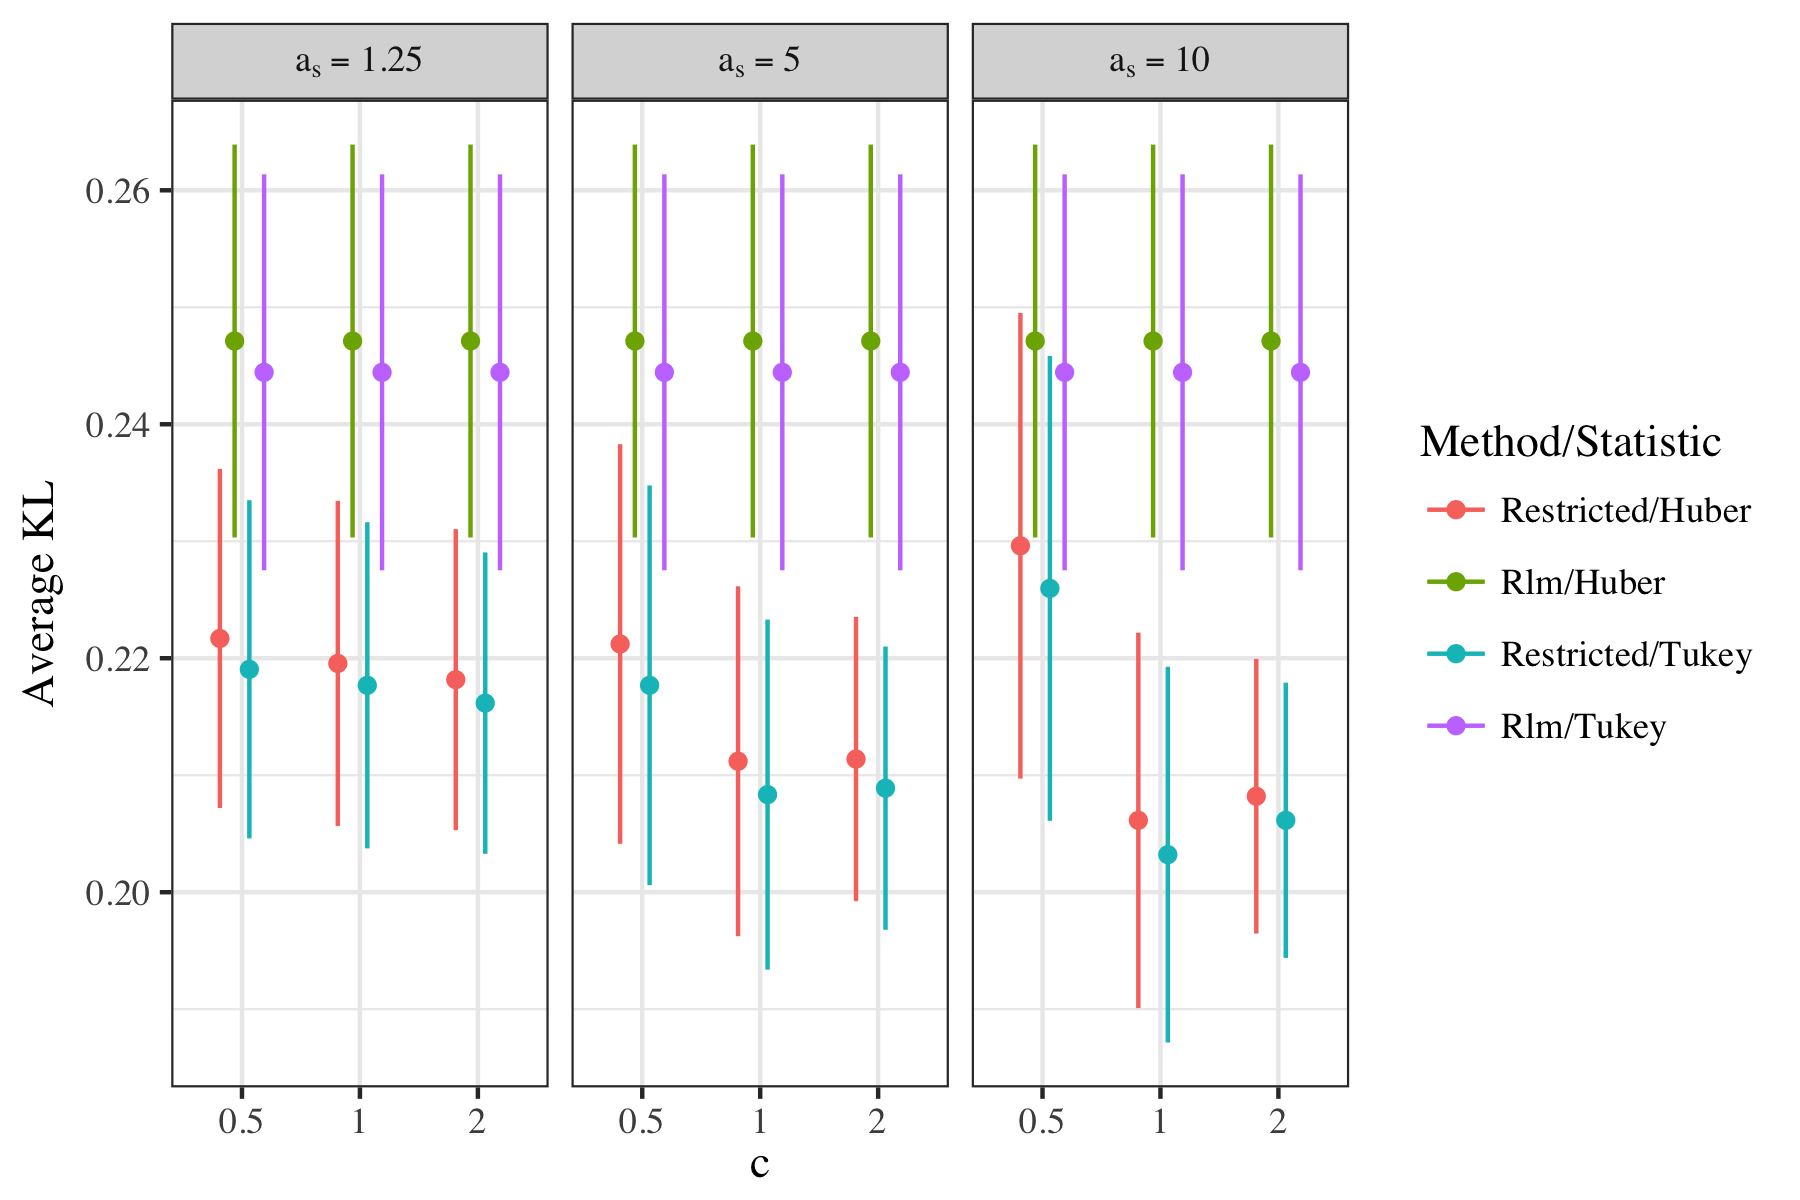
\includegraphics[scale = .3]{kl_sim2_facet_as.png}
%\end{figure}

%One explaination for the idea that 'shrinking towards smaller values' may do slightly better than shrinking toward the true value is the fact that we used default tuning parameters to define M-Estimators. For the amount of contaimination in each group, the expected value of the variance estimate (Huber's proposal 2) is larger that $\sigma^{2} = 4$. The histogram below demonstrates a sample of variaince estimates for data generated from one of the contamination groups....the estimates are consitently above 4. Thus it appears the prior mean must be smaller than the true value to get the `correct' amount of shrinkage. There is a suggestion that if the prior is too strong (large $a_{s}$), at some point, shrinking to too small a value degrades performance....which would be expected. 

%\begin{figure}[H]
%\centering
%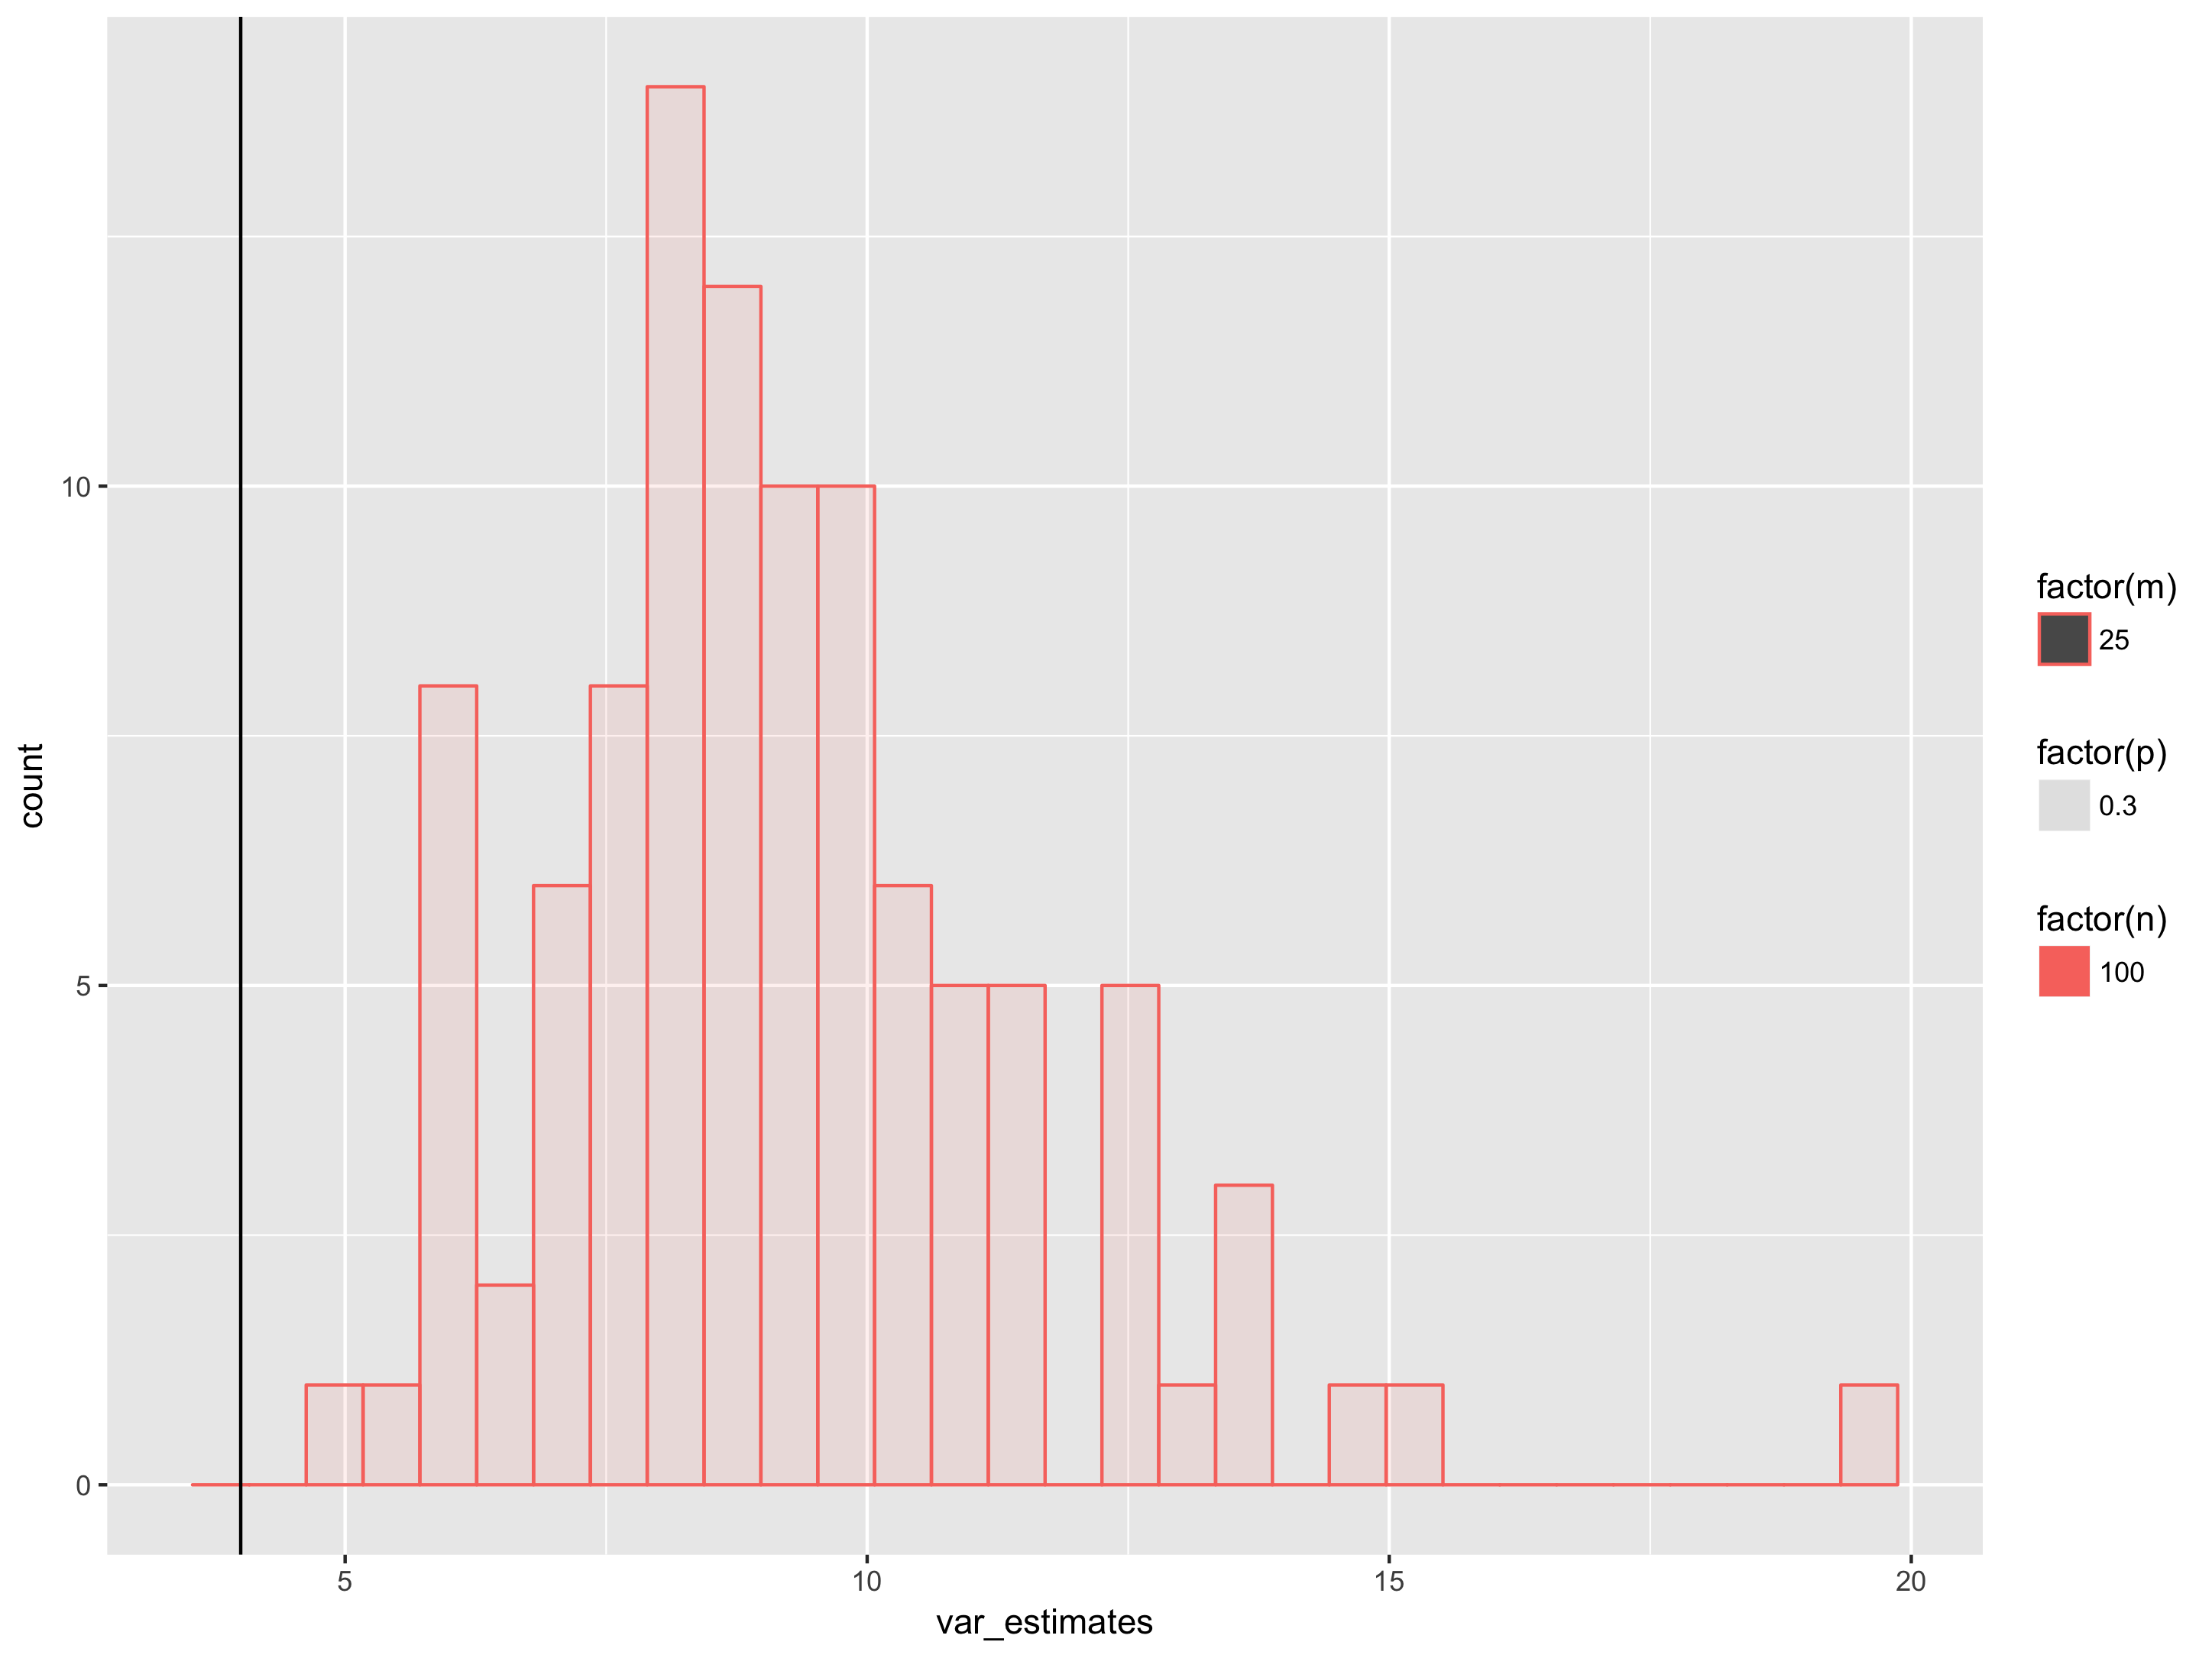
\includegraphics[scale = .3]{hist_sig2_ests.png}
%\end{figure}

%%%%%%%%%%%%%%%%%%%%%%%%%%%%%%%%%%%%%%%%%%%%%%%%%%%%%%%%%%%%
%
% Real data
%
%%%%%%%%%%%%%%%%%%%%%%%%%%%%%%%%%%%%%%%%%%%%%%%%%%%%%%%%%%%%
\section{Real Data}
\label{Real Data}
We illustrate our methods with a pair of regression models for data from Nationwide Insurance Company, which concern prediction of the performance of insurance agencies.
%The data contain many outliers and are subject to model misspecification.  
%In particular, a group of the data do not follow the same generative process as the data of interest.  It would be 
%extremely challenging to model some features of the data.  
%In our analysis, we follow the standard practice when demonstrating the benefits of robust 
%methods.  We work with a naive model for the data which ignores certain features of the problem.  We
%do this both to create a situation where all can agree that the model for the full data $\by$ is imperfect
%and to preserve the confidentiality of selected aspects of modeling done by Nationwide.  
%We wish to provide inference for the `good' portion of the data.  %The two models we fit either treat the analysis
%as a single regression or as a collection of related regressions.  % Details of the models, prior distributions, 
%and conditioning statistics are given in the next two subsections.  
%%%%%%%%%%%%%%%%%%%%%%%%
%%NW data
%%%%%%%%%%%%%%%%%%%%%%%%
%
%\subsection{Nationwide Data}
Nationwide sells many of its insurance policies through agencies which provide direct service to policy holders.  
The contractual agreements between Nationwide and these agencies vary.  Our interest is the prediction of future performance of agencies where  performance is measured by the total number of households an agency services (`household count'). 
%A serviced household is one in which at least one person living at that residence has at least one policy written through the agency. 
%We used data from previous years to build a model to forecast future household count. In particular, we use household count  as measured during a single month in $2010$, to predict household counts in the corresponding month in $2012$.  
%In particular, we use agency characteristics, as measured during a single month in $2010$, to predict household counts in the corresponding month in $2012$. The characteristics used are household count and two measurements of agency size/experience. The two measurements of agency size/experience are, roughly, the number of employed persons at the agency and the length of time the agency has been affiliated with Nationwide. 
%The household counts (response and predictor) have been square rooted to stabilize variance. 
The data a grouped by states with a varying number of agencies by state. Identifiers such as agency/agent names are removed. Likewise, state labels and agency types (identifying the varying contractual agreements) have been made generic to protect the proprietary nature of the data.
%The data are proprietary, and to mask them all variables have been individually centered and scaled and identifiers (agency/agent names and state labels) have been removed.All subsequent analysis is done on this scale.  
As an exploratory view, a plot of the square root of household count in 2012, against that in 2010 
is shown in Figure \ref{fig:ctVct} for four states. The states have varying number of agencies and  the different colors represent the varying types of contractual agreements as they stood in 2010 (`Type').  A significant number of agencies closed sometime before 2012, as represented by the $0$ counts for 2012. Among the open agencies, linear correlations exists with strength depending on agency type and state.  `Type 1' agencies open in 2012 are of special interest and one could easily subset the analysis to only these agencies, removing the others. However,  we leave them and use the data as a test bed for our techniques by fitting models that do not account for agency closures or contract type.  Our expectation is that the restricting likelihood will facilitate prediction for the `good' part of the data (i.e. open, `type 1' agencies). 

\begin{figure}[t]
\centering
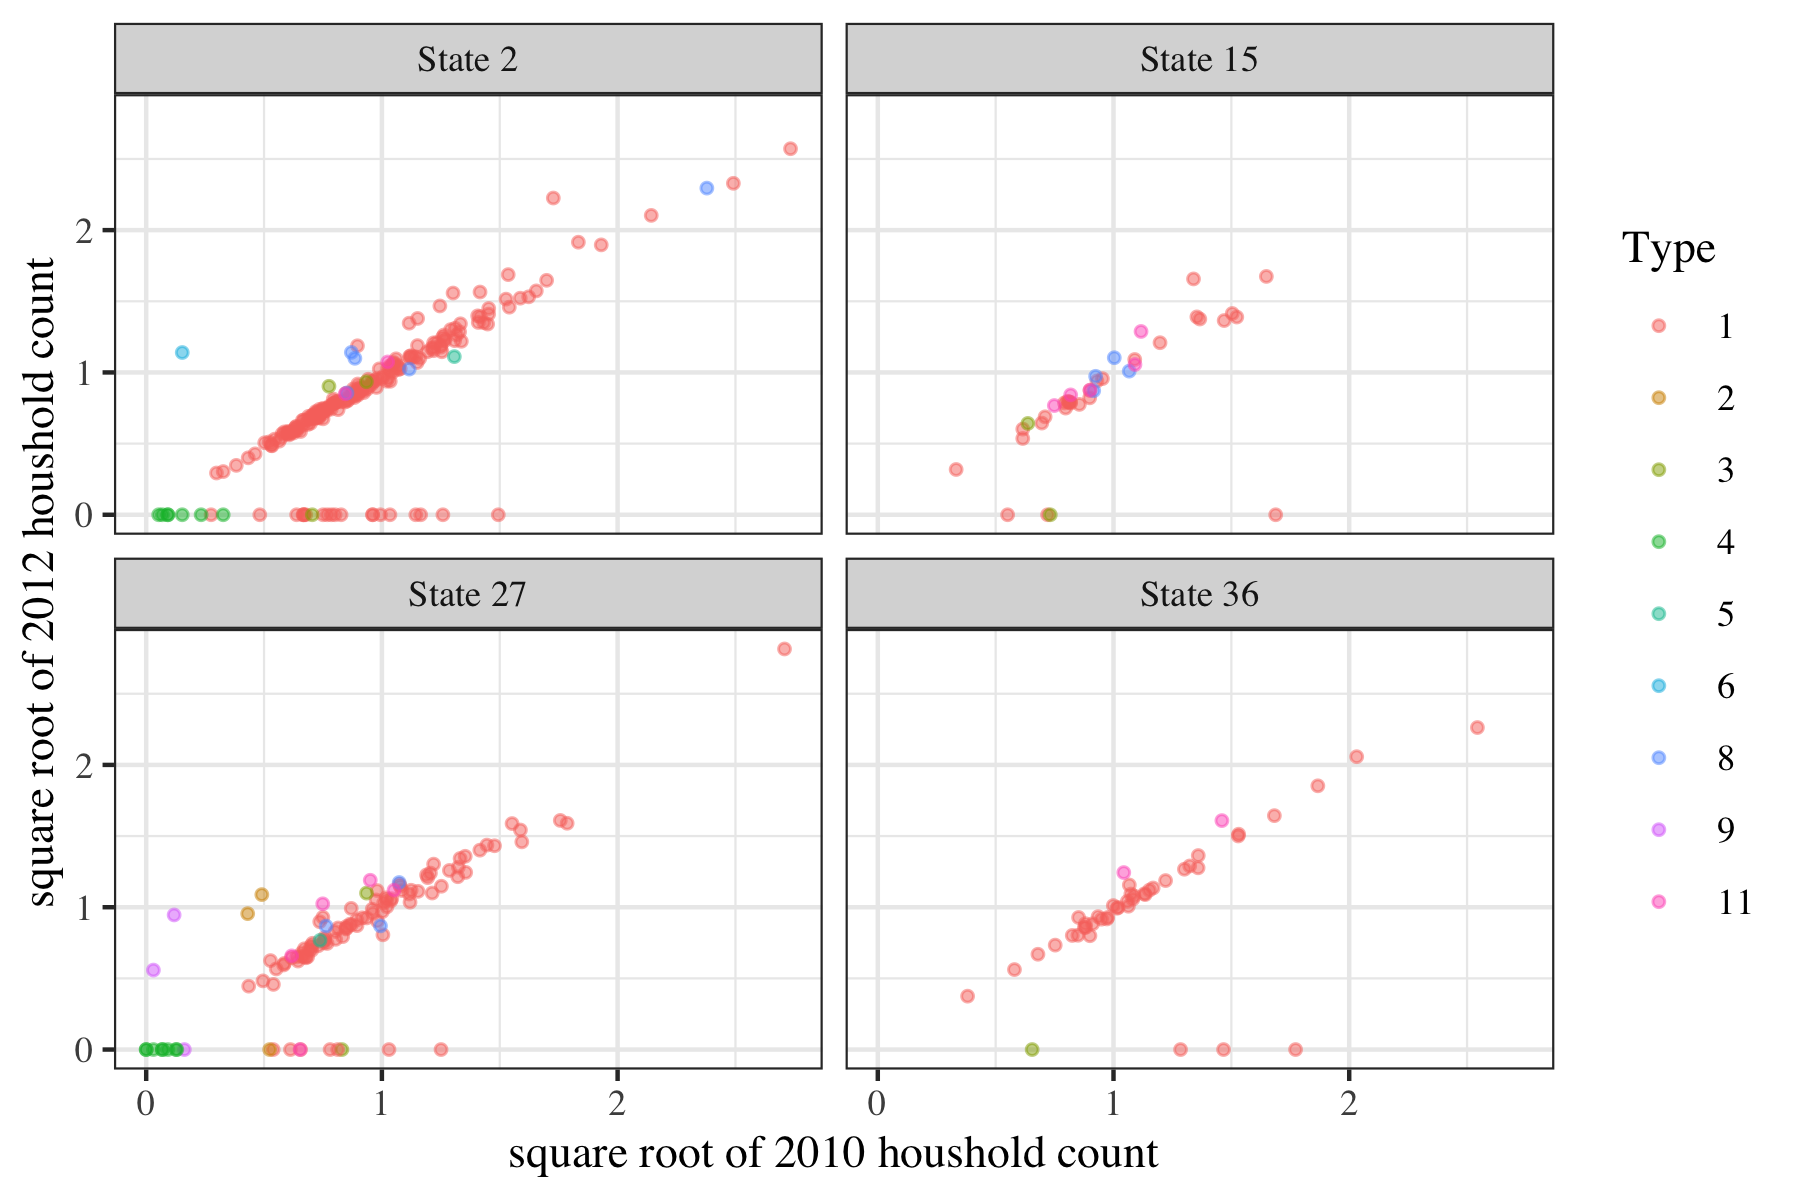
\includegraphics[width=5in]{scatter_by_state.png}
\caption{The square root of count in 2012 versus that in 2010 (after centering and scaling). The colors represent the varying contractual agreements as they stood in 2010.  Agencies that closed during the 2010-2012 period are represented by the zero counts for 2012. Scalings on the axes are purposely left off for proprietary reasons.}
\label{fig:ctVct}
\end{figure}

\subsection{State Level Regression model}
\label{regModelNW}
The first analysis considered is based on individual regressions fit separately within states.  The following normal theory regression model is used as the full model for a single state:
\begin{equation}
\label{eq:regModel}
\beta\sim N(\mu_0, \sigma^{2}_0);\ \ \sigma^2\sim IG(a_0,b_0);\ \  
y_{i}=\beta x_{i} +\epsilon_{i},\ \ \epsilon_{i}\iid N(0, \sigma^2),\ i=1,\dots, n, 
\end{equation}
%where $\beta$ is a four dimensional vector ($p=4$) of regression coefficients for the intercept, square root of count in 2010, and the two size/experience measures, and 
where $y_{i}$ and $x_{i}$ are the square rooted household count in 2012 and 2010 for the $i^{th}$ agency, respectively. 
%with covariate vector $\bx_{i}$.  Although the mean of covariates and response have been removed, we include the intercept as fitting is done on a holdout set to evaluate predictive performance.  
The hyper-parameters $a_0, b_0, \mu_0$ and $\sigma^{2}_0$ are all fixed and set from a 
robust regression fit to the corresponding state's data from the time period two years
before. Specifically, Let $\hat\beta$ and $\hat\sigma^{2}$ be estimates from the robust linear regression of 2010 counts on 2008 counts.  We fix $a_0 = 5$ and set $b_0 = \hat\sigma^{2}(a_0 - 1)$ so the prior mean is $\hat\sigma^{2}$. We set $\mu_0 = \hat\beta$ and $\sigma^{2}_0 =  n_{p}se(\hat\beta)^{2}$ where $n_{p}$ is the number of agencies in the prior data set and $se(\hat\beta)$ is the standard error of $\hat\beta$ derived from the robust regression. %The value of $f$ is varied, controlling the prior certainty on $\beta$, with smaller values corresponding to a more certain prior.  
This prior is in the spirit of the Zellner's $g$-prior \citep{zellner1986, liang2008}; in general scaling the prior variance $se(\hat\beta)^{2}$ by a factor $g$. $g = n_{p}$ is analogous to the unit-information prior \citep{kass1995reference}, with the difference that we are using a prior data set, not the current data set, to set the prior. %$f = 0.05, 0.1, 0.5, 1$ and%We fit the models separately for each $g^{*} = 0.05, 0.1, 0.5, 1$  %represent the estimate of the coefficients from this fit we  set $\bmu_0=\hat\bbeta$ and $ \Sigma_0=n\cdot \mbox{var}(\hat\bbeta)$ where here $n$ is the sample size of the prior data set.  %corresponding to  a unit information prior for $\bbeta$. 
%The hyperparameters for $\sigma^2$ are set so that the prior mean is $s^2$, the estimated variance from the robust regression, and the spread of the prior covers the range of plausible values with high probability. All values are then transformed appropriately to match the current scale of the data. In the end we take $\bmu_0=(0.18,  0.81,0.01,-0.02)^\top$ and set the mean of $\sigma^2$ to $0.014$ and standard deviation to  $0.033$. 


We compare four Bayesian models: the standard Bayesian normal theory model, two restricted likelihood models, both with simultaneous M-estimators, and a heavy-tailed model.  For the restricted likelihood methods we use the same simultaneous M-estimators as in the simulation of Section \ref{simData} adapted to linear regression.  The heavy-tailed model replaces the normal sampling density in \eqref{eq:regModel} with a $t$-distribution with $\nu = 5$ degrees of freedom. The Bayesian models are all fit using MCMC, with the restricted versions using the algorithm presented in Section \ref{highDim}.
We also fit the corresponding classical robust regressions and a least squares regression.  

\subsubsection{Method of model comparison}
We wish to examine the performance of the models in a fashion that preserves the essential features of the 
problem.  Since we are concerned with outliers and model 
misspecification, we understand that our models are imperfect and prefer to use an out-of-sample measure of fit.  
This leads us to cross-validation.  We repeatedly split the data into training
and holdout data sets; fitting the model to the training data and assessing performance on the holdout data.  

The presence of numerous outliers in the data implies that both training and validation data will contain 
outliers.  For this reason, the evaluation must be robust to a certain fraction of bad data.  
The two main strategies are to robustify the evaluation function \citep[e.g.,][]{ronchetti1997} or 
to retain the desired evaluation function and trim cases \citep{jung2014}.  Here,
we pursue the trimming approach with log predictive density for the Bayesian models and log plug-in 
maximum likelihood for the classical fits used as the evaluation function.

The trimmed evaluation proceeds as follows in our context.  The evaluation function for case $i$ in the holdout data
is the log predictive density, say
$\log(f(y_i))$, with the conditioning on the 
summary statistic suppressed.  The trimming 
fraction is set at $0 \leq \alpha < 1$. To score a method,
we first identify a base method. Denote the predictive density under this method by $f_{b}(y)$.  Under the base method, $\log(f_{b}(y_i))$ is computed for each case in the 
holdout sample, say $i = 1, \ldots, M$.  Order the holdout sample according to the ordering of $\log(f_{b}(y_i))$ and denote this
ordering by $y_{(1)}^b, y_{(2)}^b, \dots, y_{(M)}^b$. That is, for $i<j$
$\log(f_{b}(y_{(i)}^b))<\log(f_{b}(y_{(j)}^b))$. All of the methods are then scored on the holdout sample with the mean trimmed log marginal pseudo likelihood, 
\[TLM_b(A) = (M - [\alpha M])^{-1} \sum_{i=[\alpha M]+1}^{M}
    \log(f_A(y_{(i)}^b)),\]
 where $f_A$ corresponds to the predictive
 distribution under the method ``A'' being scored.  In other words, the $[\alpha M]$ observations with the smallest values of $\log(f_{b}(y))$ are 
removed from the validation sample and all of the methods are scored using only the
remaining $M - [\alpha M]$ observations. This process is advantageous to the base method since the smallest scores from this method are guaranteed to be trimmed.  A method
that performs poorly when it is the base method is discredited.  %For a complete evaluation, we allow each method
%to appear as the base method.  For brevity, we present only a selection of results in our subsequent analyses.  

\subsubsection{Comparison of predictive performance}
%Model performance is assessed using the mean and standard deviation of the TLM 
%across $K = 50$ different splits into training and holdout samples. 
`Type 1' agencies are of special interest to the company and so the evaluation of the TLM is done on only holdout samples of `Type 1', wheres the training is done on agencies of all types. This is intended to demonstrate the robustness properties of the various methods. 
%First, we include all observations
%in each validation sample to calculate TLM for each split. We then
%repeat the evaluation using only certain subsets of the validation
%sample that are of special interest. Subsets include open agencies,
%open `Type 1' agencies, and `Type 1' agencies. For brevity, we include
%results for the `Type 1' agencies only. As noted, assessing model
%predictions on this set of agencies is of special interest to the
%company.  A range of training sample sizes was used and we include
%results from $n=25,100,1000,$ and $2000$ out of a total of $3180$ agencies. 
%The trimming fraction, $\alpha$, ranges from $0$ to $0.3$. A classical robust regression to the prior data assigns zero weight to around $16\%$ of observations; in essence removing these from the analysis. This informed the range of trimming fractions chosen.  
%In practice, we would set $\alpha$ slightly larger than $0.16$.  
Models are fit to four states labelled State 2, 15, 27, and 36, with $n = 222, 40, 117,$ and $46$, representing a range of sample sizes. Training sample sizes are taken to be $.25n$ and $0.50n$ with holdout evaluation done on the remaining (`Type 1`) samples. The average $TLM_b(A)$ over $K = 50$ training/holdout samples for the four states and seven methods are shown in Figure \ref{fig:tlm} where the base model is the Student - t model and $\alpha = 0.3$. Similar results are observed for other base models, with this one being most advantageous to the Student - t model. The error-bars are plus/minus one standard deviation of the average $TLM_b(A)$ over the $K = 50$  training/holdout samples. It is clear the normal Bayesian model used as the base model (Normal) and the classical ordinary least squares fits (OLS) have poor performance, as expected, due to the significant amount of outlier contamination in the data. In comparing are restricted methods to their corresponding classical methods, there is small, but consistent improvement across the states and training sample size. For state 2, the largest state with $n = 222$, the restricted and classical robust methods have similar performance especially for larger training sample size. This reflects the diminishing effect of the prior as the sample size grows. Notably, the Student - t model performs poorly in comparison for this state. The predictive distribution explicitly accounts for heavy-tailed values, resulting in poorer predictions of the `good` data (i.e. the Type 1 agencies). Likewise, for State 27, another larger state, the Student-t model is outperformed by our restricted methods.   For the other states, the Student-t performs similarly to our restricted methods for the smaller states (State 15 and 36) and smaller training size (25\% of the sample). However, the performance is worse for the larger training size (50\% of the sample). Intuitively, as more data is available for fitting, more outliers appear and the heavy-tailed model compensates for them by assuming they come from the tails of the model; detrimental for prediction. The relative performance of the models are similar for various values $\alpha$. Figure \ref{fig:tlmbyAlpha} shows the results for one state (State 27) with training sample size $0.5n$ as an example. 



%A mixture model could replace the heavy-tailed model. We assert it is more difficult to refine a mixture model in this setting reflecting the different types of outliers including the zero counts and agency types. The appeal of the restricted likelihood (and the classical robust approaches) is the avoidance of refining the model to capture (potentially transient) outlier generating mechanisms. Instead, the modeler focuses on estimating quantities of interest via statistics $T(\by)$. The improvement in our restricted likelihood versions over the classical robust fits is due to the informative prior distributions. In this case, similar data from previous years was used to formulate the prior. Like all Bayesian methods, performance is affected by the prior and it is important the prior accurately reflects the prior state of knowledge. 

\begin{figure}[t]
\centering
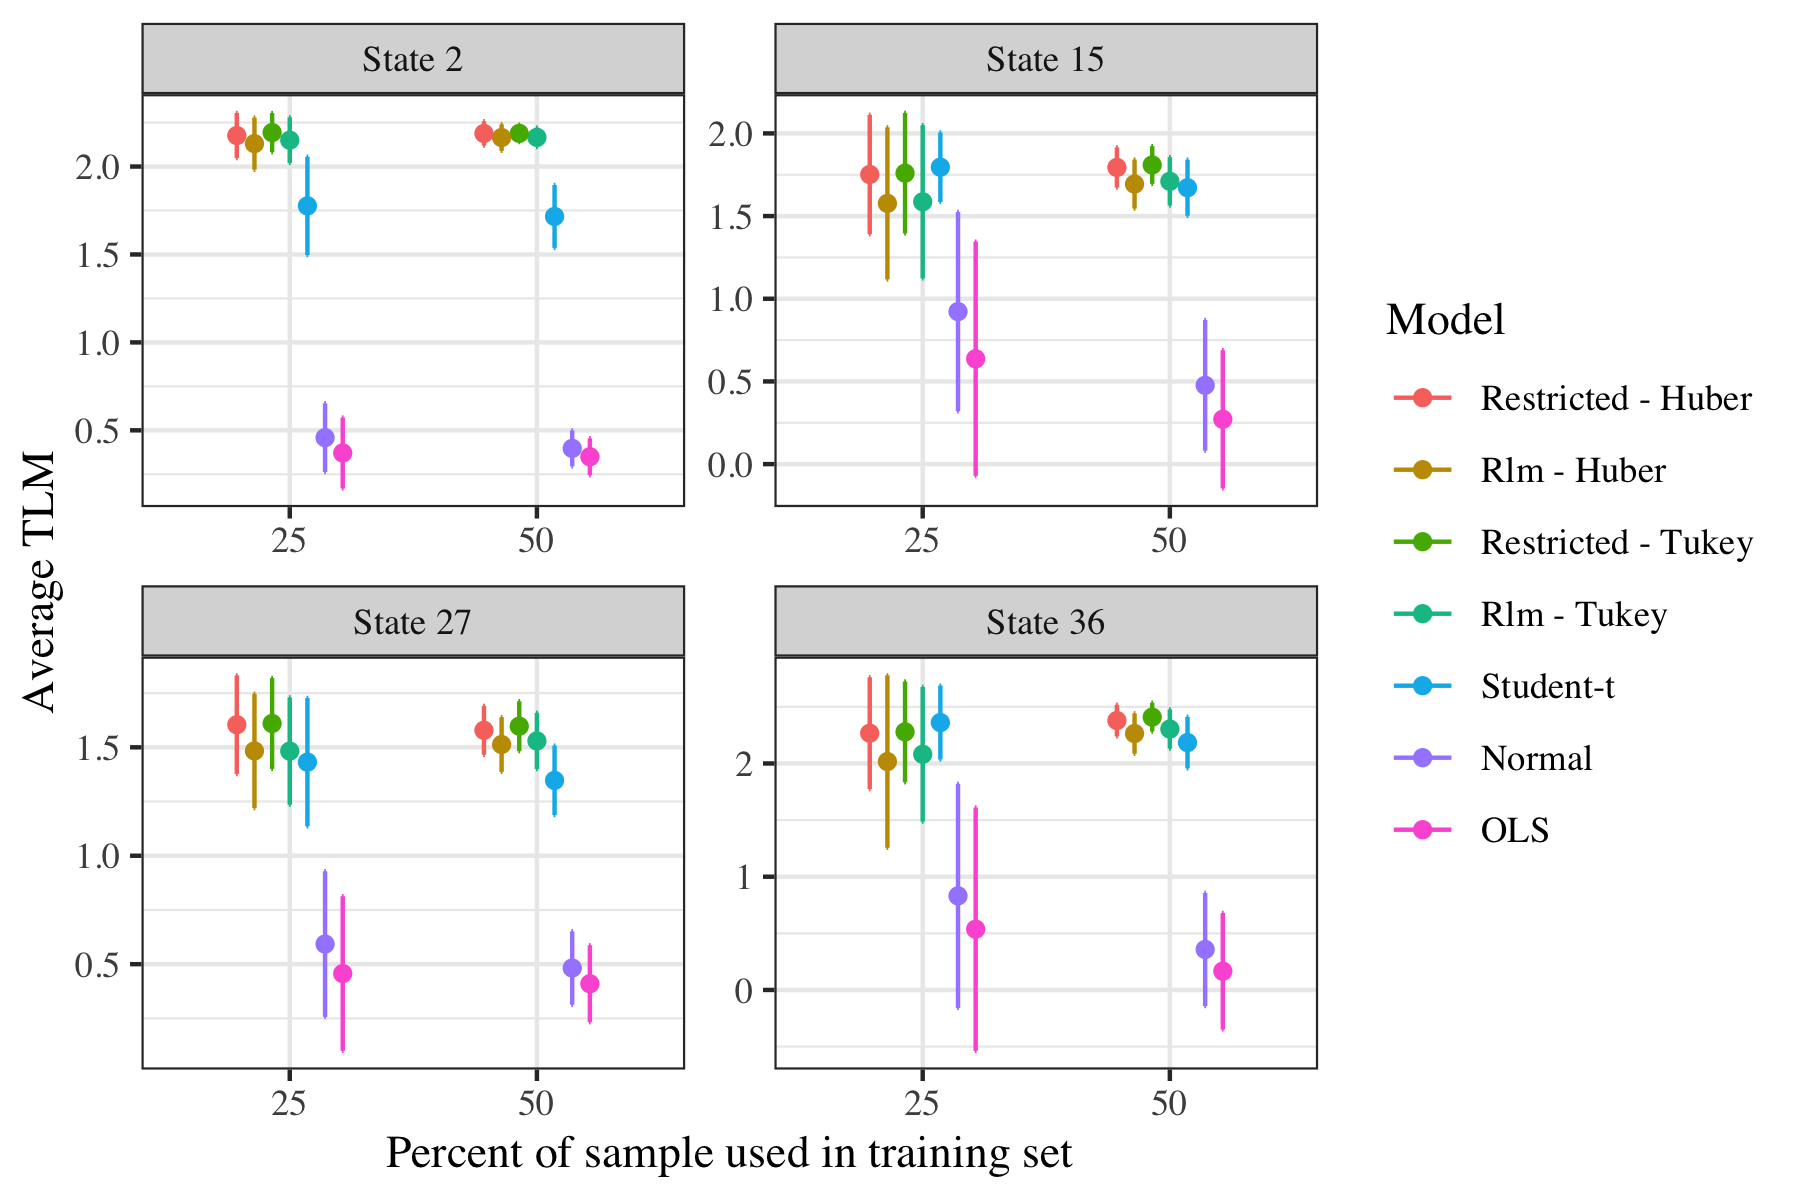
\includegraphics[width=6in]{tlm_base_Student-t.png}
\caption{Average TLM plus/minus one standard deviation over $K = 50$ splits into training and holdout samples. The panels are for the different states  2, 15, 27, and 36, with $n = 222, 40, 117,$ and $46$, respectively. The horizontal axis is the percent of $n$ used in each training set. The color corresponds to the fitting model. }
\label{fig:tlm}
\end{figure}

\begin{figure}[t]
\centering
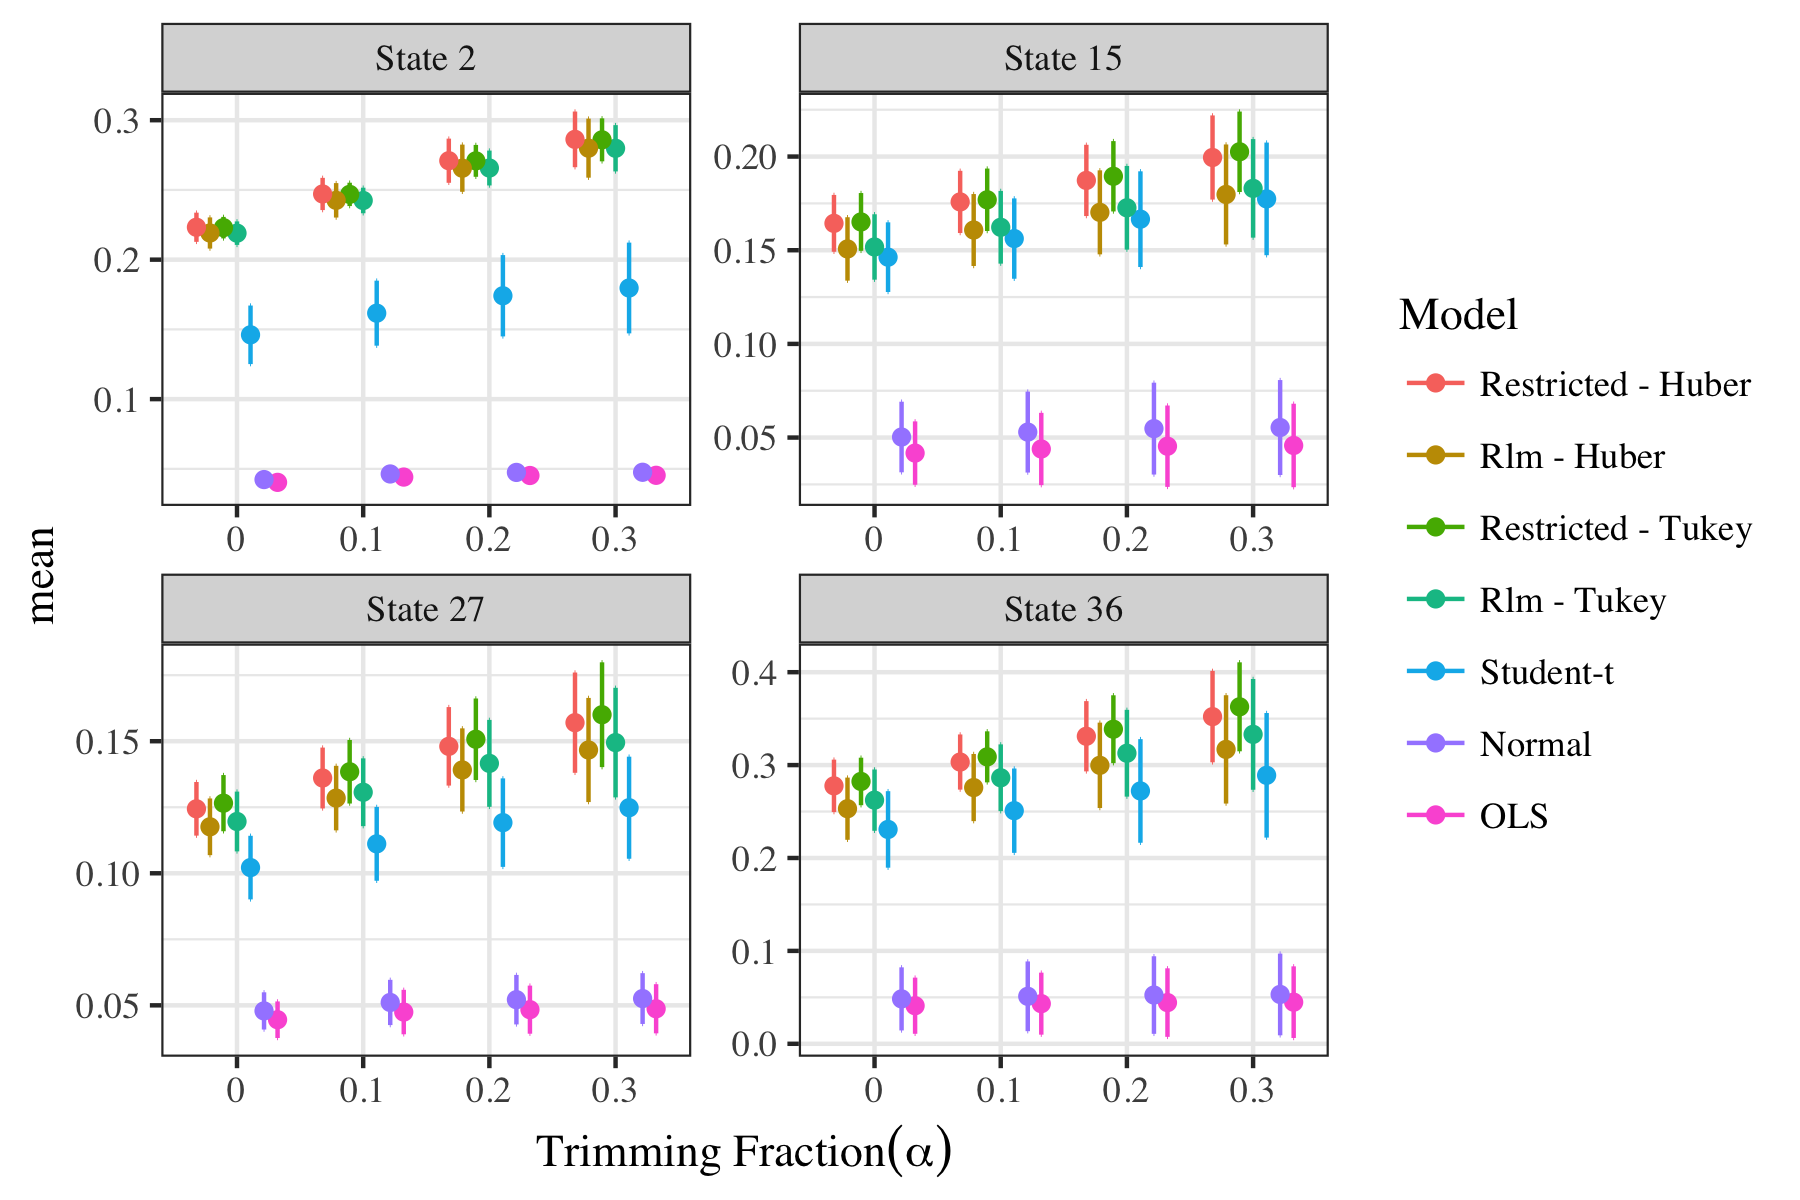
\includegraphics[width=6in]{tlm_base_Student-tbyTrimming.png}
\caption{Average TLM plus/minus one standard deviation over $K = 50$ splits into training and holdout samples for several values of the trimming fraction $\alpha$. The training sample size used is $0.5n$.}
\label{fig:tlmbyAlpha}
\end{figure}

%\begin{sidewaysfigure}
%\centering
%\captionsetup{justification=centering}
%%\subcaptionbox{}{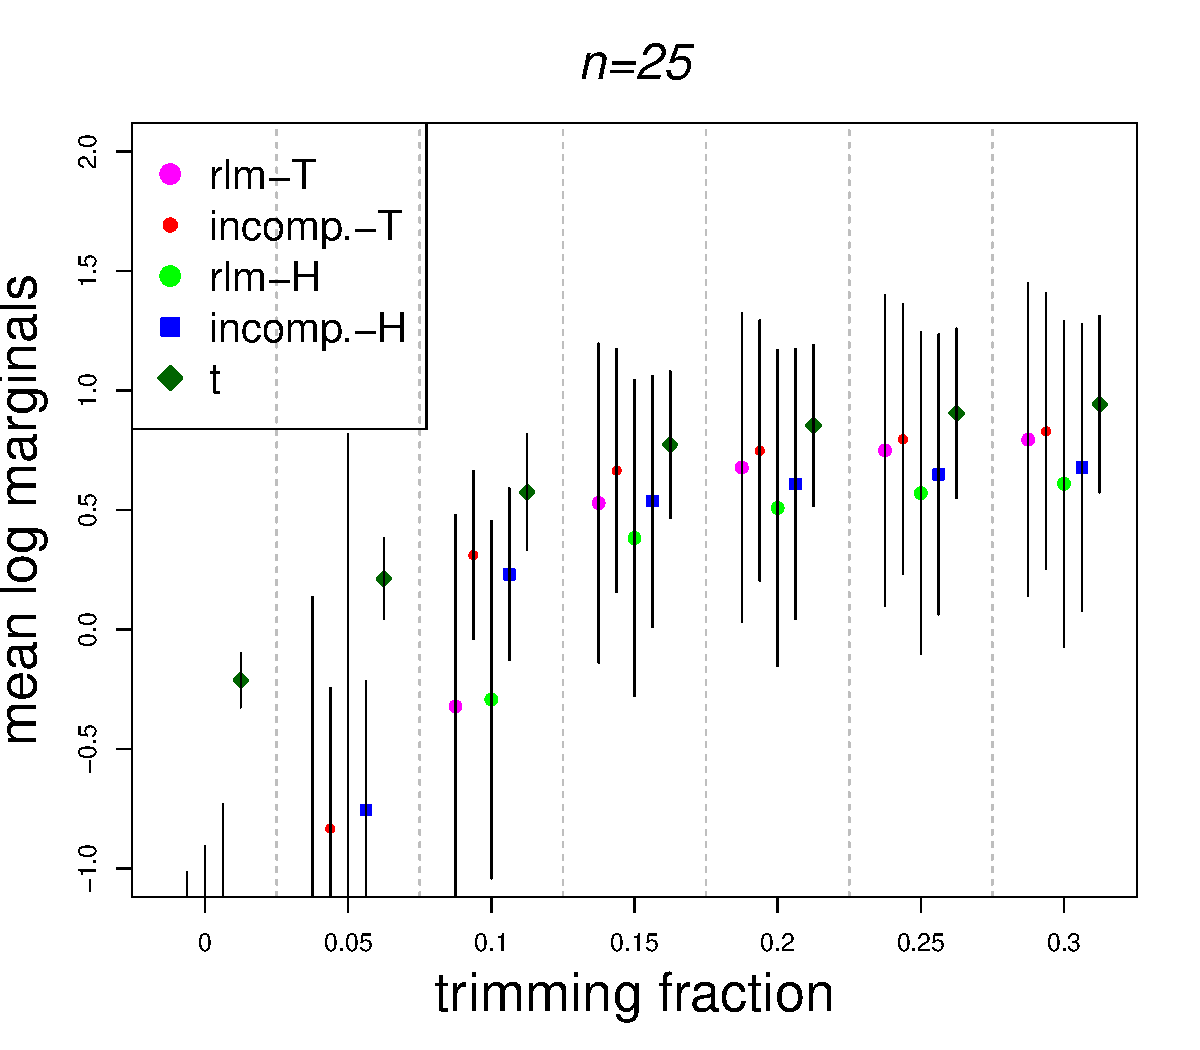
\includegraphics[width=\textwidth,page=1]{logMargType1AgenciesBaseModelt}}\quad
%%\subcaptionbox{}{\includegraphics[width=\textwidth,page=2]{logMargType1AgenciesBaseModelt}}\quad
%%\subcaptionbox{}{\includegraphics[width=\textwidth,page=3]{logMargType1AgenciesBaseModelt}}
%\subcaptionbox{}{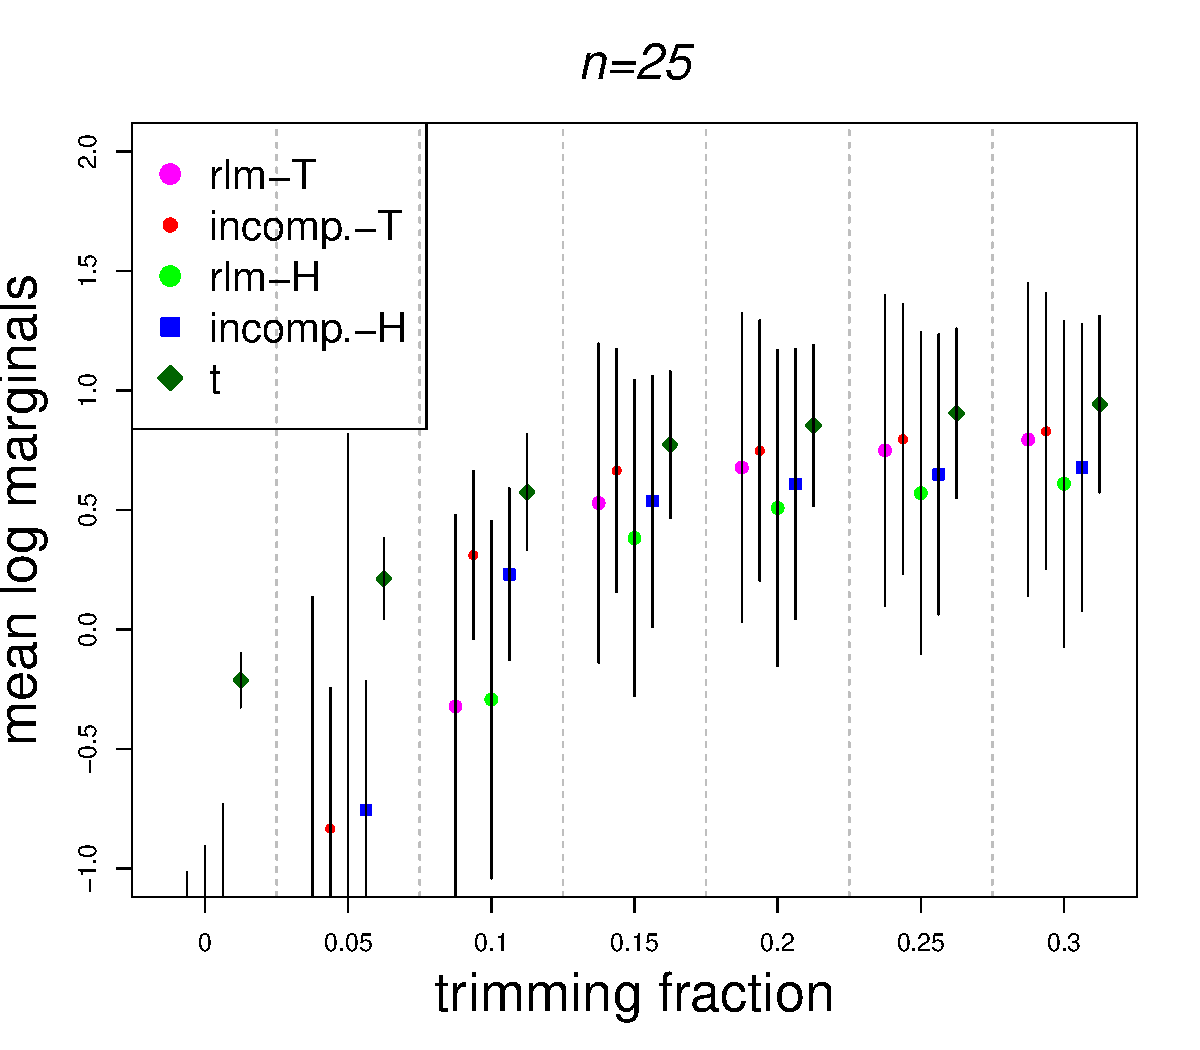
\includegraphics[width=3.4in,height=3.3in, page=1]{logMargType1AgenciesBaseModelt}}\quad
%\subcaptionbox{}{\includegraphics[width=3.4in,height=3.3in,page=2]{logMargType1AgenciesBaseModelt}}\quad
%\subcaptionbox{}{\includegraphics[width=3.4in,height=3.3in,page=3]{logMargType1AgenciesBaseModelt}}
%\caption{Model evaluation for `Type 1' agencies for training sample
%  sizes of $n=25,100$, and $1000$. The $t$-model is used as the base
%  method to compute TLM. Plotted are the mean TLM for each model
%  against the trimming fraction across the $100$ cross-validation
%  samples. Error bars correspond to one standard deviation of TLM
%  above and below the mean. Models are labeled with the following
%  abbreviations: `rlm' corresponds to a classical robust fit, `restr.'
%  corresponds to our restricted likelihood method, and `t' corresponds to the
%  heavy-tailed $t$-distribution model. The letters `T' and `H'
%  appearing after `rlm' and `restr.' correspond to the use of  Tukey's
%  and Huber's $\psi$ respectively.  
%}
%\label{fig:Type1Marg}
%\end{sidewaysfigure}
%


%Model evaluation for `Type 1' agencies is shown in Figure
%\ref{fig:Type1Marg} for training sample sizes $n=25, 100,$ and $1000$.
%The $t$-model is used as the base
%  method to compute TLM.
%The models pictured are: classical robust regression with Tukey's $\psi$ function (rlm-T), restricted likelihood with Tukey $\psi$ (restr.-T), classical robust regression with Huber's $\psi$ function (rlm-H), restricted likelihood  with Huber's $\psi$ (restr.-H), and the thick tailed $t$-model (t). The normal theory models perform poorly due to the numerous outliers
%and are left out of the figures. Appearing in the figures are the mean TLM across
%validations set for each model and each trimming fraction, $\alpha$ (along the $x$-axis). The error bars depicted are one standard deviation of the TLM above and below the mean.  The range of the vertical axis is chosen to enhance important features and as a result, some evaluation measures extend below this range. In particular, the restricted likelihood methods perform poorly if no trimming is done; reflecting that these methods are not intended to fit well to outliers. Recall that we expect about 15-16\% outliers in the validation sets, thus trimming fractions slightly larger than this amount are needed in order to assess fits to the `good' data. For $n=25$, the thick tailed model  prevails across trimming fractions, although less so for $\alpha\geq 0.15$. For sample sizes as low as $n=100$, the restricted likelihood methods outperform the heavy-tailed model with the Tukey version performing the best.   
%The stronger performance of restricted likelihood based on Tukey's method and the t model is to be expected, as many of the 
%residuals are so extreme that trimming is better than winsorizing (as Huber's method effectively does).  
%As expected, with enough data,  the Bayesian methods and their classical counterparts perform similarly, although there
%is a persistent slight edge in favor of the Bayesian restricted likelihood methods.  We attribute this advantage to the weakly informative
%prior distribution which pulls the estimates slightly toward better values.  The similarity occurs as early as $n=100$. 
%
 
\subsection{Hierarchical regression model}
\label{hierRegNW}
The previous analysis treated states independently. A natural extension is to  reflect similar business environments between states using a hierarchical regression. The proposed model is:
\begin{align}
%\begin{split}
\label{eq:hierModel}
&\beta\sim N_p(\mu_0, a\sigma_0^{2});\ \ 
\beta_j\iid N_p(\beta, b\sigma_0^{2}); \ \  
\sigma_j^2\sim IG(a_0,b_0);  & \\ \nonumber
& y_{ij}=x_{ij}\beta_j+\epsilon_{ij},\ \ \epsilon_{ij}\iid N(0, \sigma_j^2),\ i=1,\dots, n_j,\ j=1,\dots, J &
%\end{split}
\end{align}
where $y_{ij}$ is the $i^{th}$ observation of square rooted household count in 2012 in the $j^{th}$
state, $n_{j}$ is the total number of agencies in state $j$, and $J$ is
the number of states. $x_{ij}$ is the square rooted household count in 2010 and $\beta_j$ represents the individual regression coefficient vector for state $j$. As with the state level regression, the parameters $\mu_0$,
$\sigma^{2}_0$, $a_0$, and $b_0$ are fixed. Specifically we set $\mu_{0} = \hat\beta$ and $n_{p}\hat\sigma^{2}_{0}$ where $n_{p}$ is the number of observations in the prior data set and the estimates are from a robust fit of $y_{ij}=x_{ij}\beta+\epsilon_{ij}$ on the prior data. For $\sigma^{2}_{j}$, $a_{0}=5$ and $b_{0} = \bar\sigma^{2}(a_{0} -1)$ where $\bar\sigma^{2}$ is a weighted (by number of observation) average of individual estimates of each $\sigma_{j}^{2}$ from the previous data set. We constrain $a+b=1$
in an attempt to partition the total variance between the individual
$\beta_j$'s and the overall $\beta$. We take $b\sim
\text{beta}(v_1,v_2)$. Using the prior data set, we assess the
variation between individual estimates of the $\beta_j$ to set $v_1$
and $v_2$ to allow for a reasonable amount of shrinkage. To allow for
dependence across the $\sigma_j^2$ we first take
$(z_1,\dots,z_J)\sim N_J(\mathbf{0}, \Sigma_\rho)$ with
$\Sigma_\rho=(1-\rho)\mb{I}+\rho \mb{1}\mb{1}^{\top}$. Then we set
$\sigma^2_j=H^{-1}(\Phi(z_j))$ where $H$ is the cdf of an
$IG(a_0,b_0)$ and $\Phi$ is the cdf of a standard normal. This results in the specified marginal distribution, while
introducing correlation via $\rho$. We assume $\rho\sim
\text{beta}(a_\rho,b_\rho)$ with mean $\mu_\rho=a_\rho/(a_\rho+b_\rho)$ and precision
$\psi_\rho=a_\rho+b_\rho$. The parameters $\mu_\rho$ and
$\psi_{\rho}$  are given beta and gamma distributions, with fixed hyperparameters. More details on setting prior parameters are given in the appendix. 

Using the same techniques as in the previous section, 
we fit the normal theory hierarchical model above, a thick-tailed $t$ version with $\nu = 3$ d.f., and two restricted likelihood versions (Huber's and Tukey's) of the model.  For the incomplete restricted methods, we condition on robust regression estimates fit separately within each state. We also fit classical robust regression counterparts and a least squares regression separately within each state. Hierarchical models naturally require more
data and so we include states having at least 25 agencies resulting in 22 states and $n = \sum_{j} n_{j} =  3180$ total agencies. For training data we take a stratified (by state) sample of size $3180/2 = 1590$ where the strata sizes are $n_{j}/2$ (rounded to the nearest integer). The remaining data is used for a holdout evaluation using TLM computed separately within each state: $TLM_b(A)_{j} = (M_{j} - [\alpha M_{j}])^{-1} \sum_{i=[\alpha M_{j}]+1}^{M_{j}} \log(f_A(y_{(i)j}^b))$ where $y_{(1)j}^b, y_{(2)j}^b,..., y_{(M_{j})j}^b$ is the ordering of the $M_{j}$ holdout observations within state $j$ according to the log marginals under the base model $b$. For the non-Bayesian models,  $f_A(y_{(i)j}^b$ is estimated using plug-in estimators for the parameters for state $j$. $TLM_b(A)_{j}$ is computed for each state for $K=50$ splits into training and holdout sets. For each fit the Bayesian models are fit using MCMC with the restricted versions applying the algorithm laid out in Section \ref{BayesLinMod} adapted to the hierarchical setting as described in Section \ref{simData}.

%We digress briefly to note that for the restricted likelihood methods no additional computational strategies outside of those discussed in Section~\ref{highDim} are needed to fit the hierarchical models described here. Since we condition on statistics which are computed within each state, the model's conditional independence between the states allows the data augmentation described earlier to be performed independently within each state.  Updates of hyperparameters follow conventional MCMC procedures.  We note that different types of statistics could be chosen for each state, if desired, allowing for a large amount of flexibility.  

The average over states, $\overline{TLM}_b(A)$ for each of the $K$ repetitions is summarized in Figure
\ref{fig:hierTLM} for several trimming fractions using the Student-t as the base model. The points are the average of the $\overline{TLM}_b(A)$ over the $K$ repetitions with errorbars plus/minus one standard deviation over $K$. Again, the normal theory fits, both Bayesian and classical, perform poorly.  We also see, that even using it as the base model to compute TLM, the Student-t doesn't perform well in comparison to the robust regressions. On average, the classical robust regressions fit separately within each state slightly outperform the restricted likelihood hierarchical models. The hierarchical model does however, reduce variance in predictions at the cost of an increase in bias induced by the prior distributions. This can be seen in Figure \ref{fig:hierTLMsd} which shows the standard deviation of $\overline{TLM}_b(A)$ relative to the mean over the $K=50$ repetitions. The results displayed are for the two restricted likelihood versions of the hierarchical model and their corresponding robust regression models fit separately within each state. It is clear that the hierarchical model reduces sample-to-sample variation in comparison the the classical robust model counterparts.  

\begin{figure}[t]
\centering
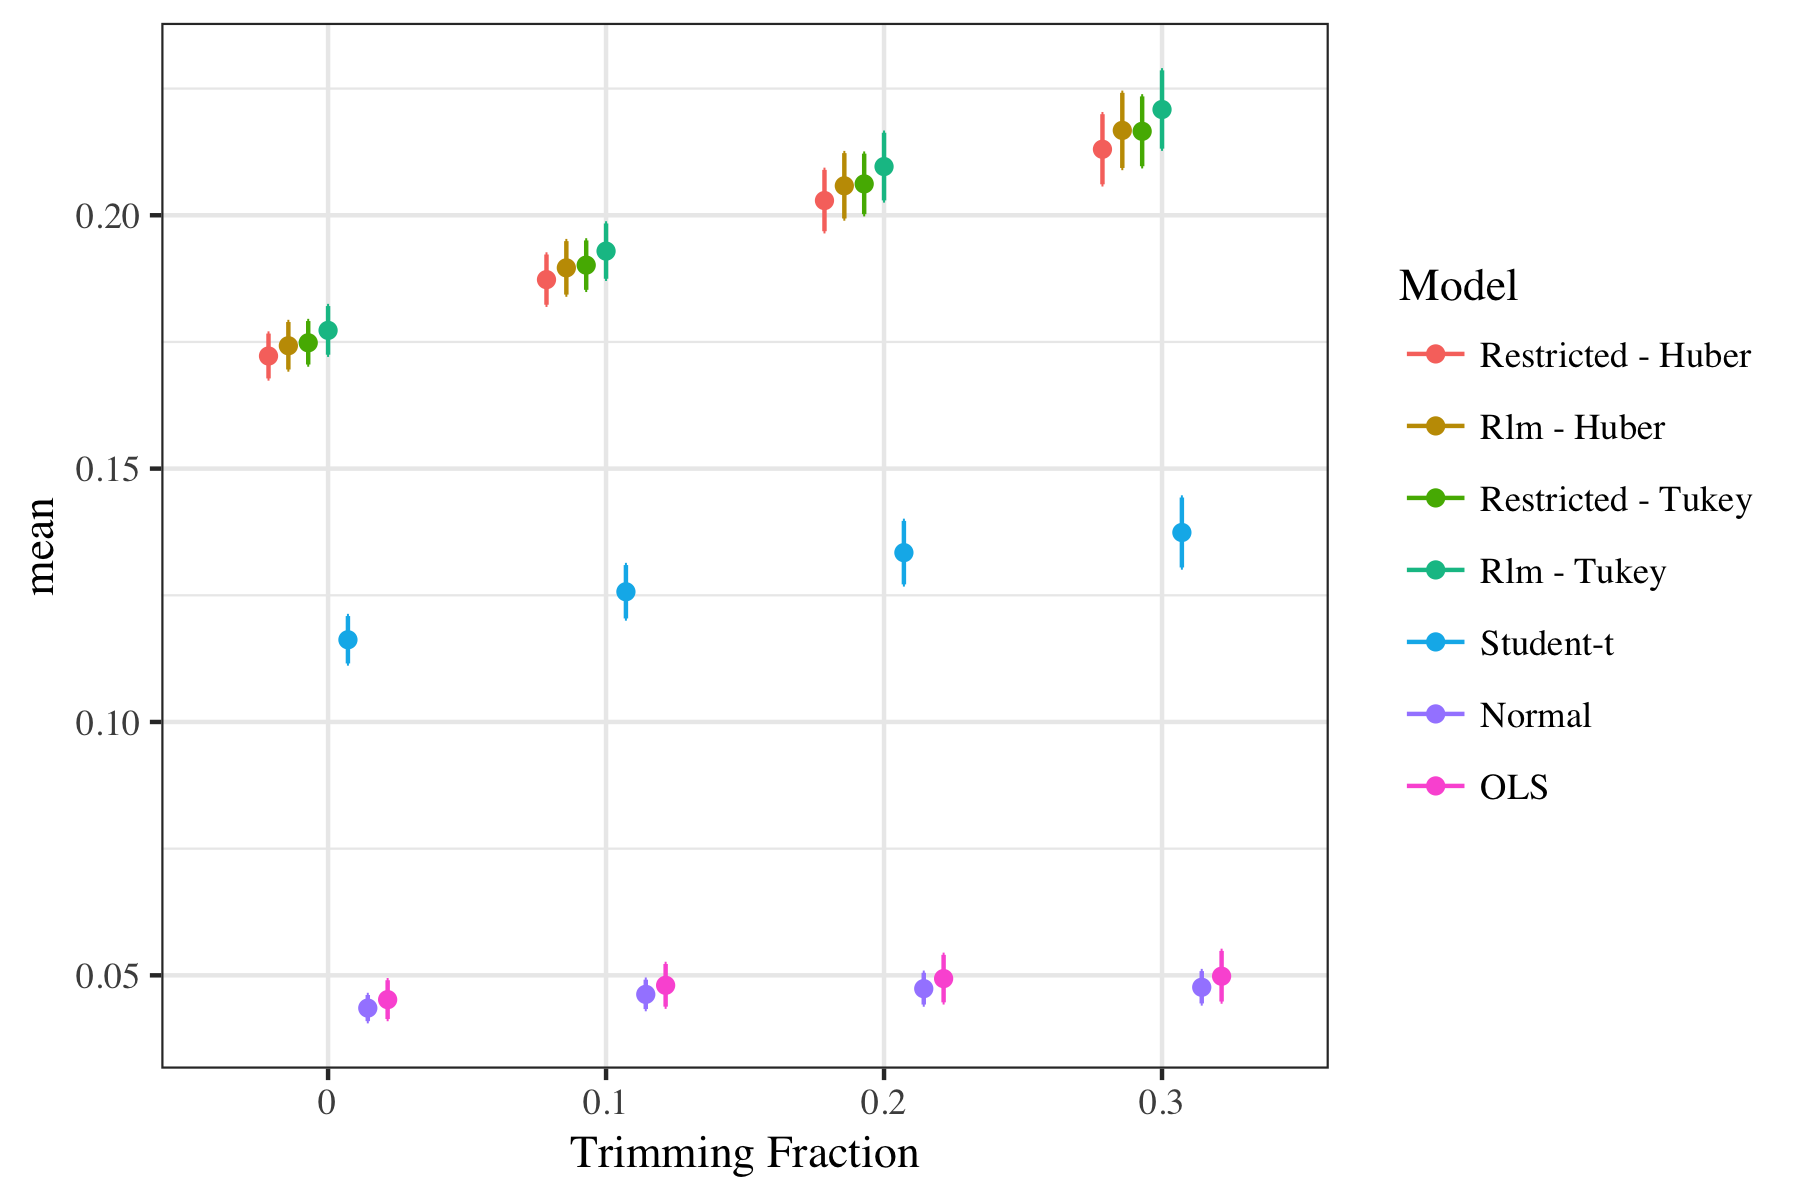
\includegraphics[width=6in]{hier_average_tlm.png}
\caption{Hierarchical model results: $\overline{TLM}_b(A)$  plus/minus one standard deviation over $K = 50$ splits into training and holdout sets for several values of the trimming fraction $\alpha$.}
\label{fig:hierTLM}
\end{figure}

\begin{figure}[t]
\centering
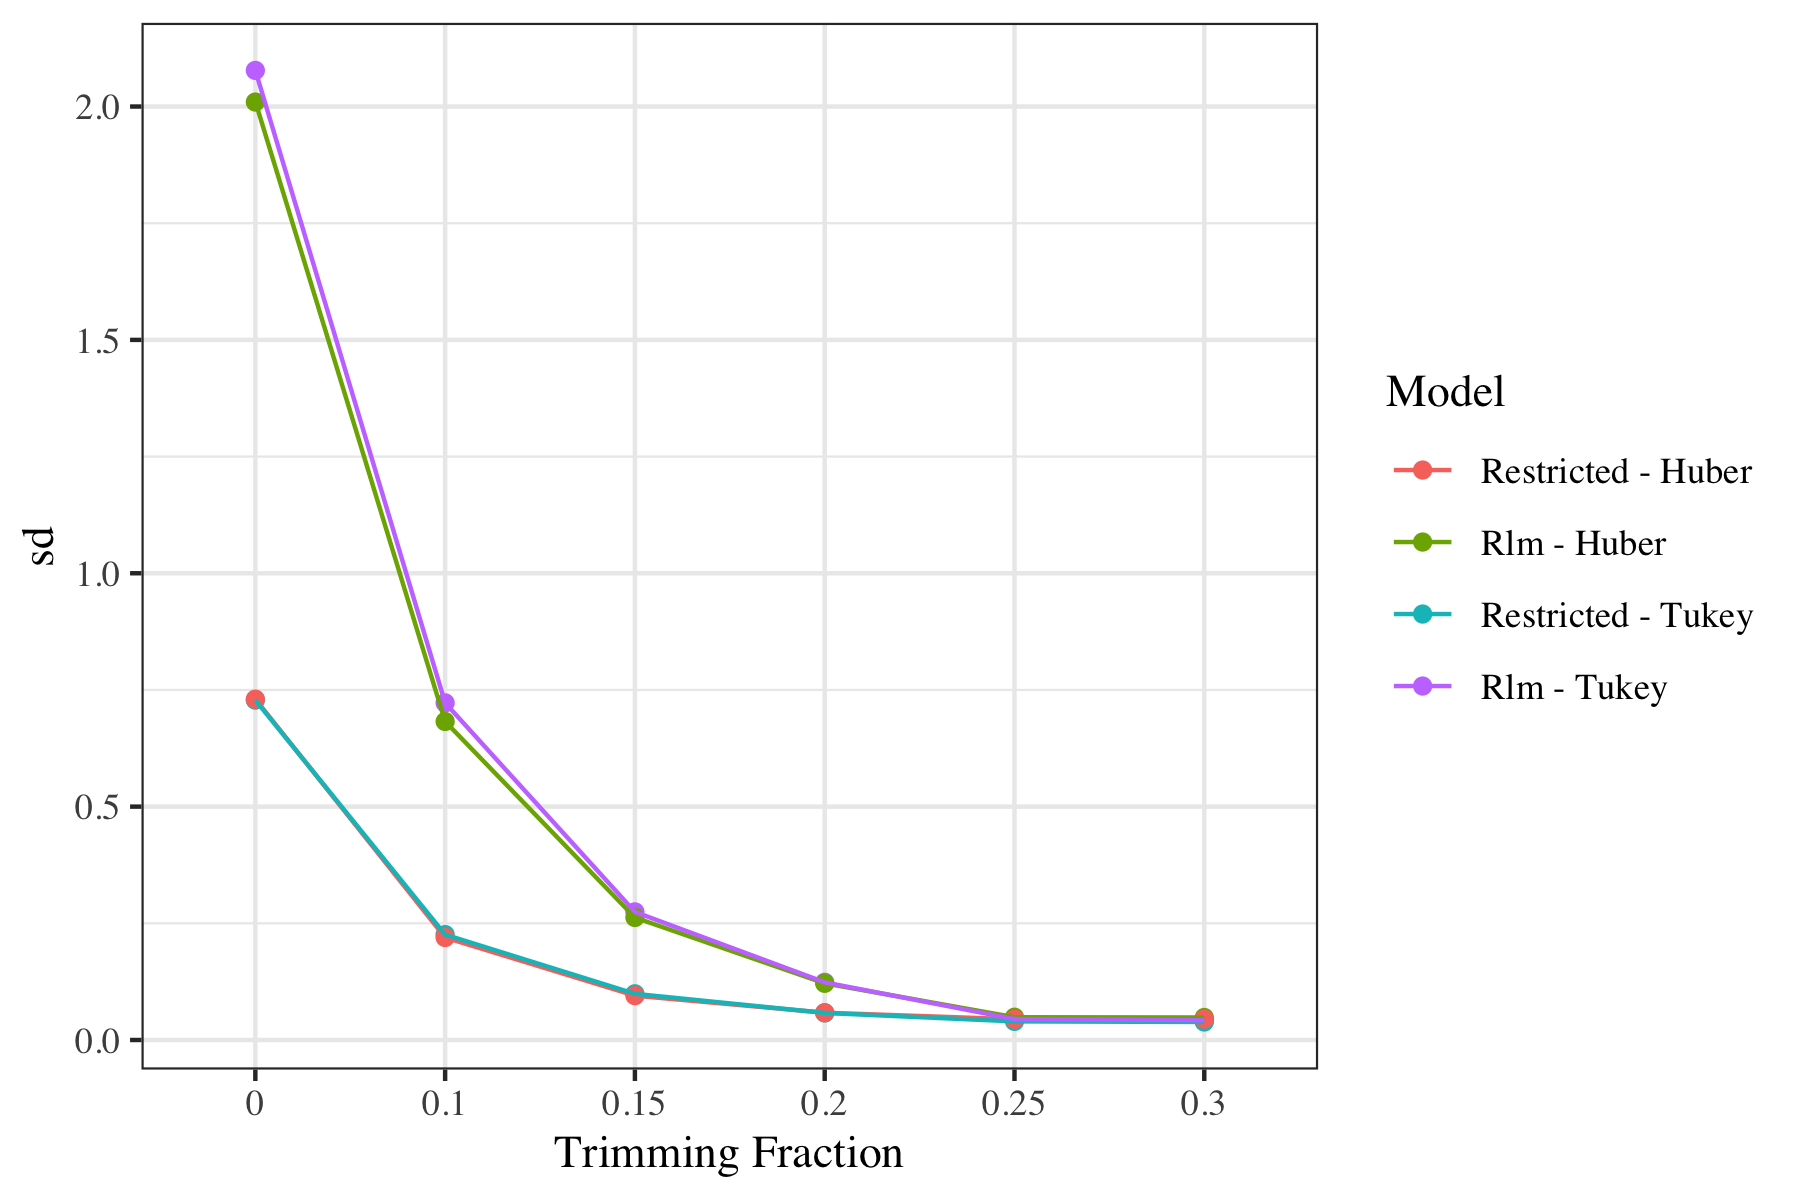
\includegraphics[width=6in]{hier_sd_tlm.png}
\caption{Hierarchical model results: standard deviation of $\overline{TLM}_b(A)$ relative to the mean over $K = 50$ splits into training and holdout sets for several values of the trimming fraction $\alpha$. Results are given for the two restricted likelihood versions of the hierarchical model and their corresponding robust regression models fit separately within each state.}
\label{fig:hierTLMsd}
\end{figure}

It is also interesting to examine the individual results within each state. Figure \ref{fig:hierTLMstate} summarizes ${TLM}_b(A)_{j}$ for each state where the points and errorbars are the averages and plus/minus one standard deviation over the $K = 50$ repetitions. The results are only given for the models using Tukey's M-estimators since, in general, these models performed the best.  The states are ordered along the x-axis according to number of agencies with the state (shown in parentheses). In several of the smaller states, the restricted hierarchical model performs better on average with similar performance between the models in most of the larger states; a reflection of the decreased influence of the prior. It is clear that the prior is having the affect of pooling information across states; this is beneficial for average TLM in some states but detrimental in others. However, for each state, the sample-to-sample variance in smaller under the restricted likelihood model. This is shown in Figure \ref{fig:hierTLMstateSD} of the standard deviation of ${TLM}_b(A)_{j}$ relative to the mean for each. The general trend in the figure is that the standard deviation decreases as the number of observations within a state increases. Additionally, the differences between the restricted likelihood hierarchical and classical robust version is larger for smaller states with virtually identical standard deviations for the larger states. 

 
\begin{figure}[t]
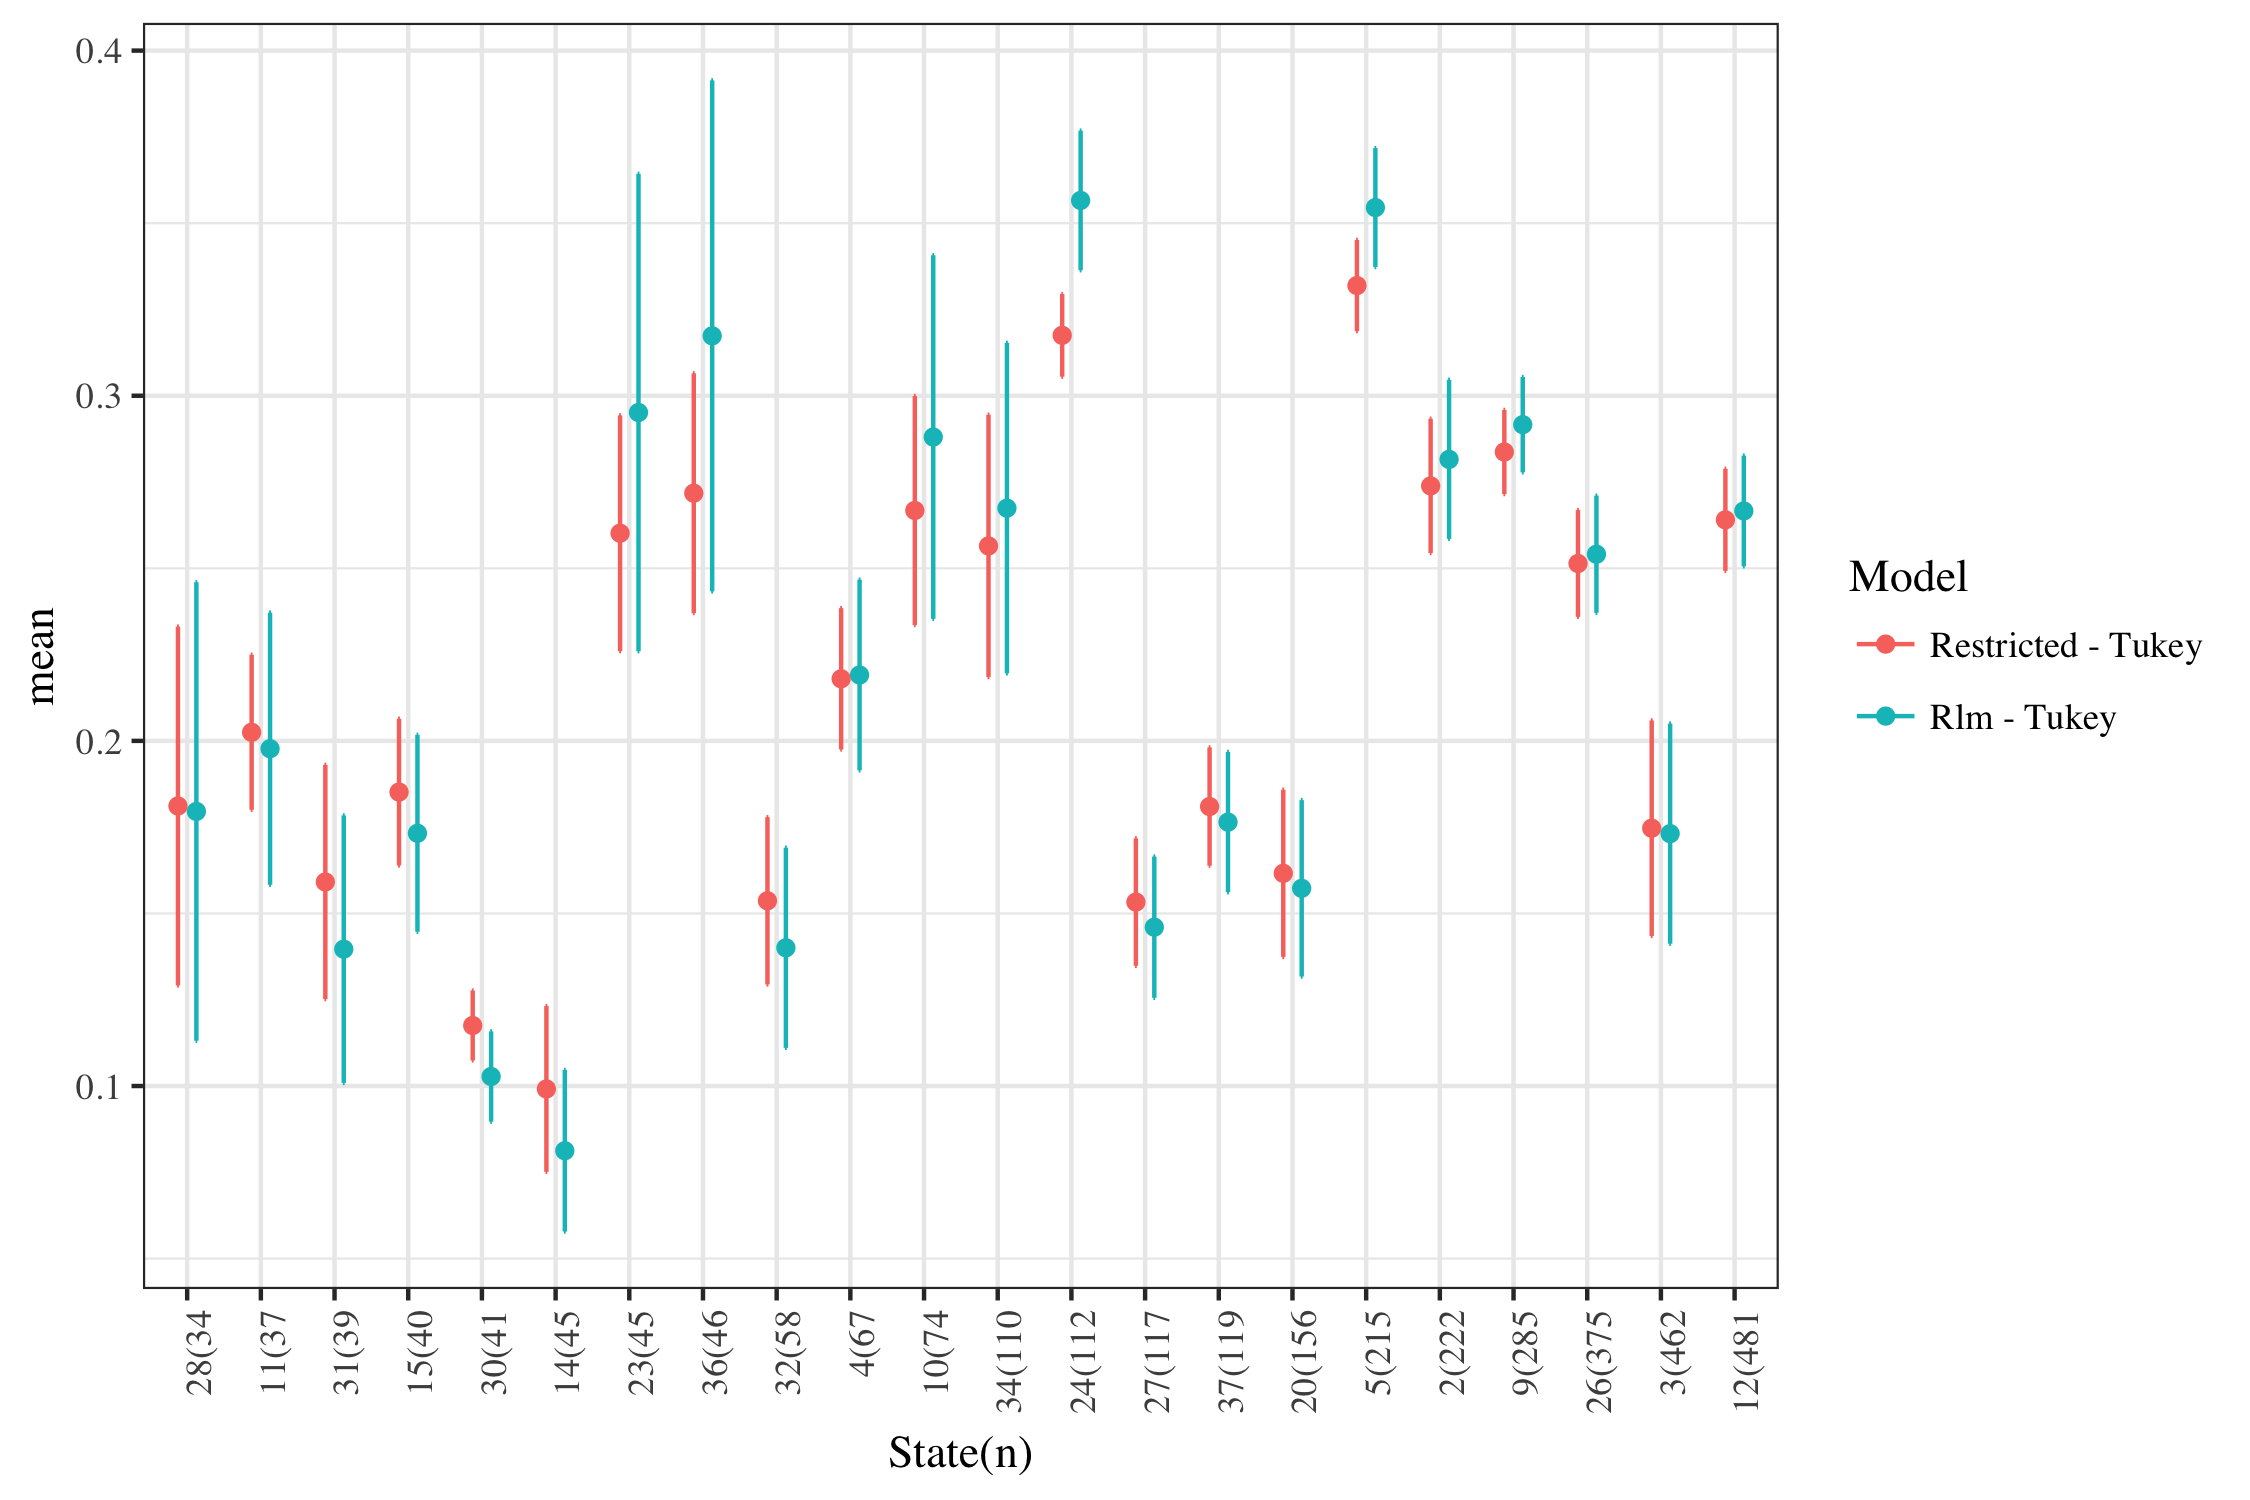
\includegraphics[width=7in]{hier_ave_tlm_state.png}
\caption{Hierarchical model results: ${TLM}_b(A)_{j}$  plus/minus one standard deviation over $K = 50$ repetitions for each state and $\alpha = 0.3$. The states are ordered along the x-axis according to number of agencies with the state (shown in parentheses). Results displayed are for the robust models using Tukey's M-estimators.}
\label{fig:hierTLMstate}
\end{figure}

\begin{figure}[t]
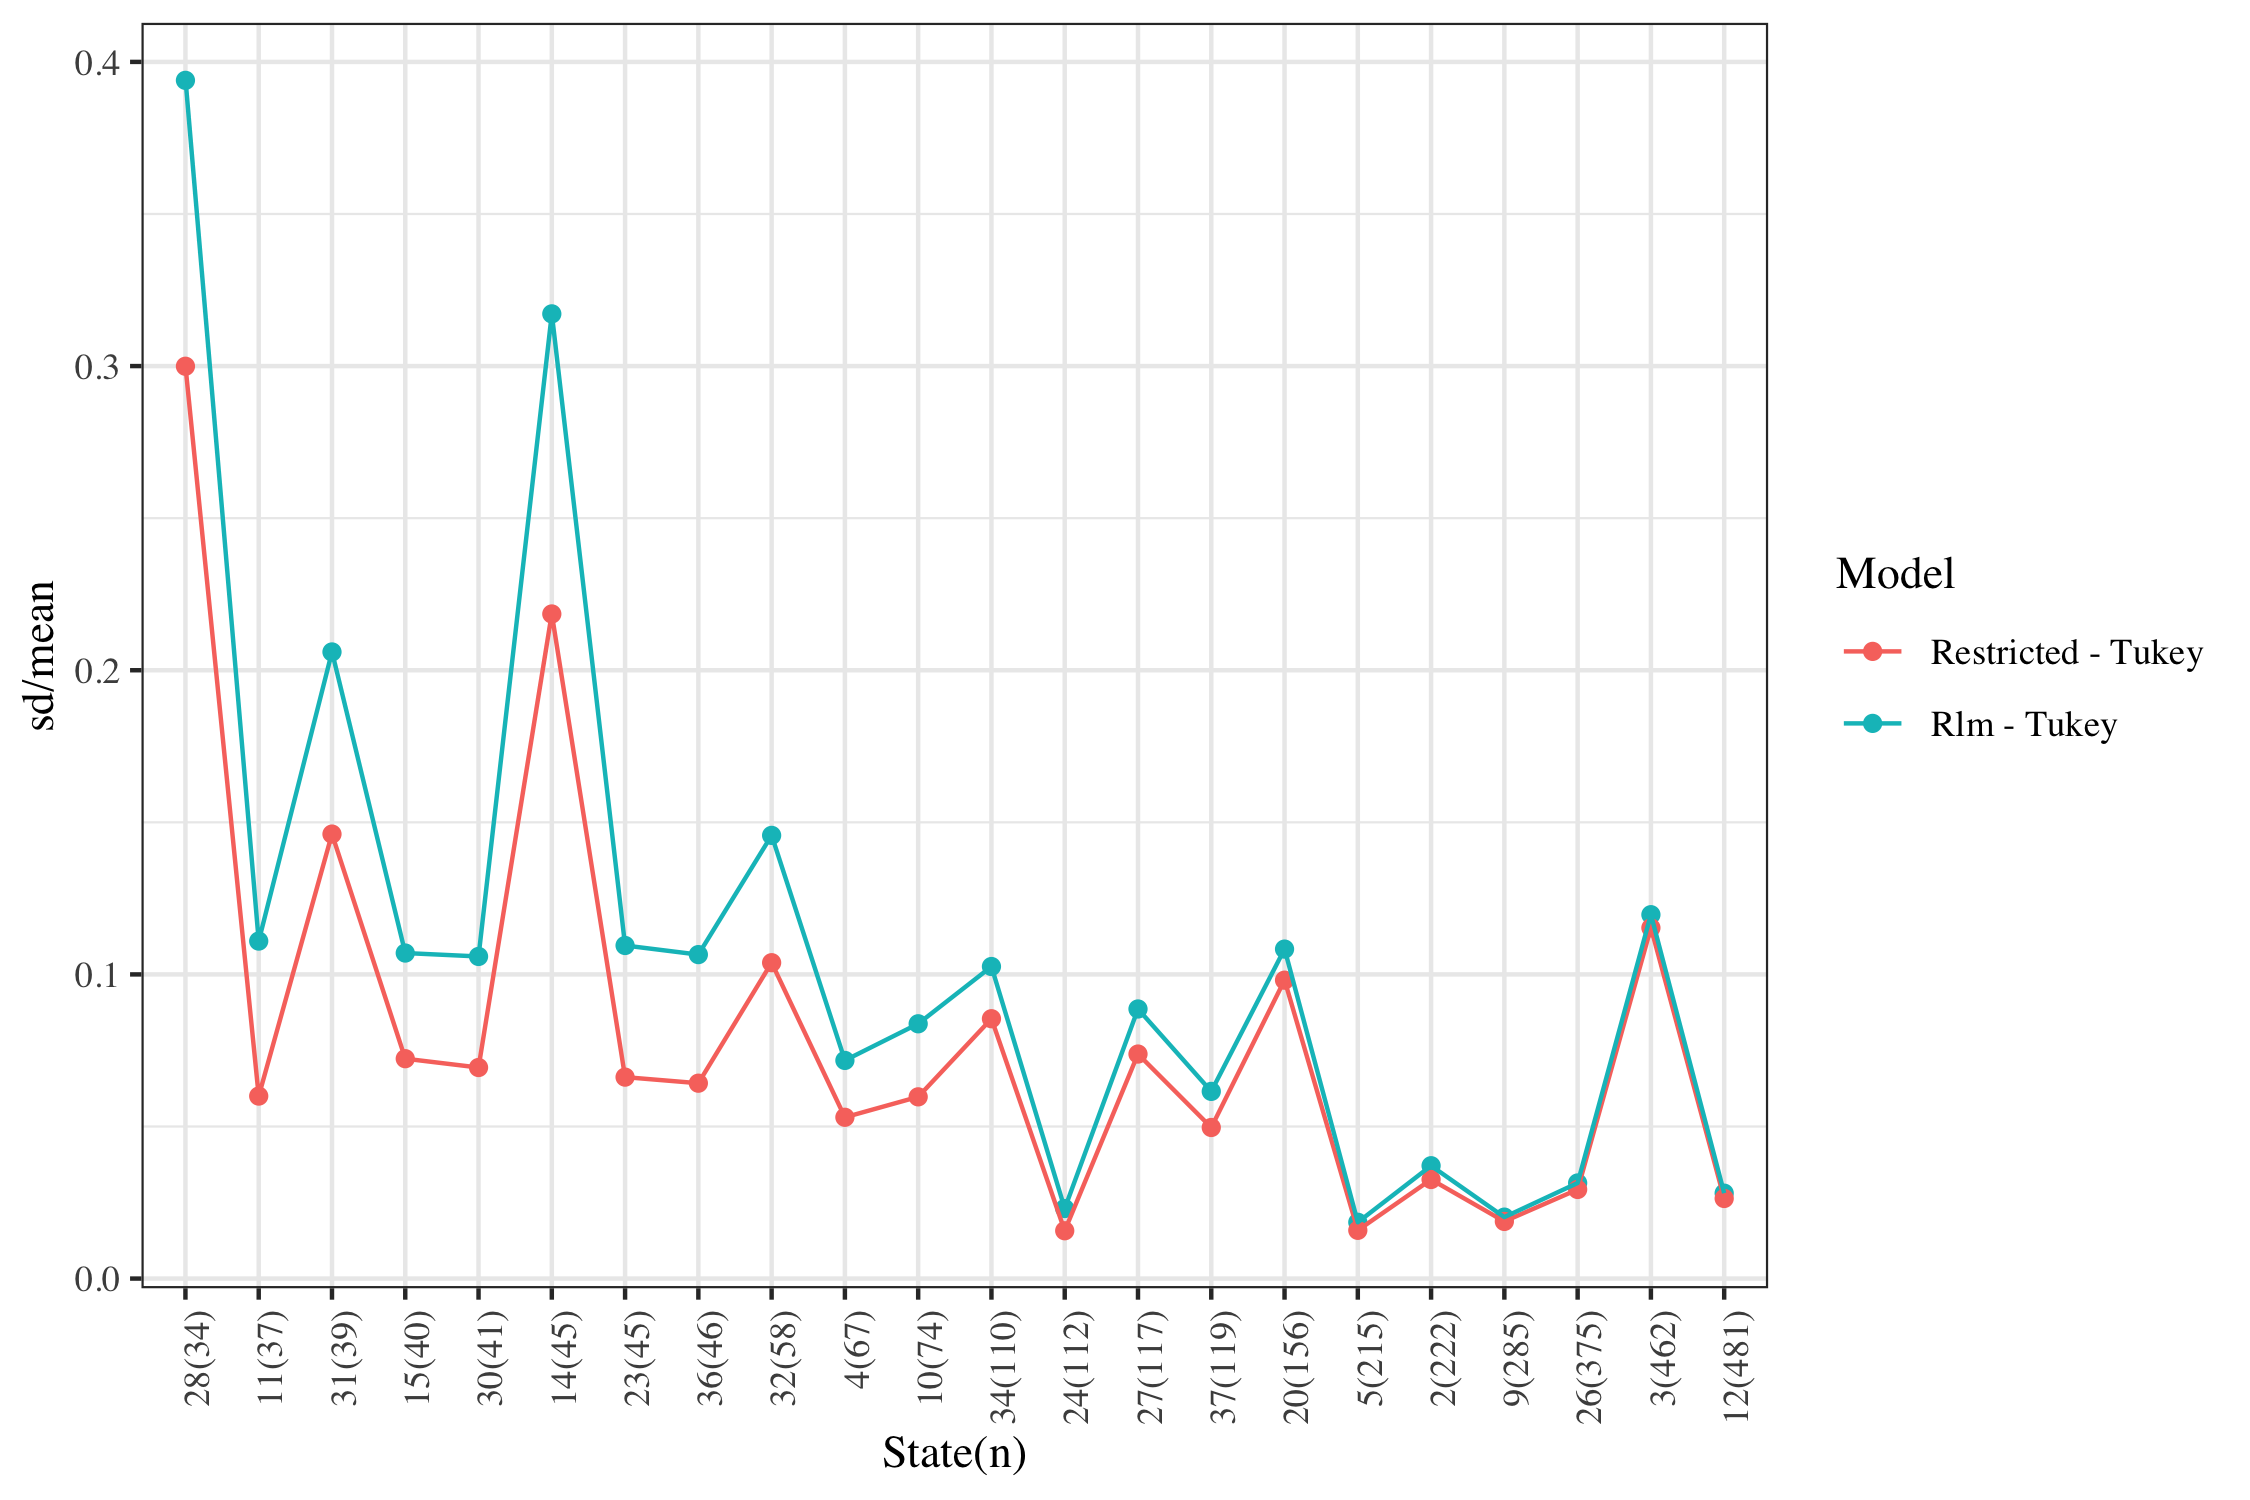
\includegraphics[width=7in]{hier_sd_tlm_state.png}
\caption{Hierarchical model results: Standard deviation of ${TLM}_b(A)_{j}$  relative to the mean over $K = 50$ repetitions for each state and $\alpha = 0.3$. The states are ordered along the x-axis according to number of agencies with the state (shown in parentheses). Results displayed are for the robust models using Tukey's M-estimators.}
\label{fig:hierTLMstateSD}
\end{figure}



%We see that the restricted likelihood with Tukey's estimator performs best in each case (assuming sufficient trimming). Huber's version also tops the thick tailed model for $n=2000$.  The Bayesian restricted likelihood fits considerably outperform their respective individual classical robust fits for training size of $n=1000$. This observation remains, though marginally so, for $n=2000$. The advantage of the hierarchical models seen here is due to the pooling of information across states, resulting in better predictive performance as compared to both the thick tailed competitor as well the respective classical fits.



%\begin{sidewaysfigure}[t]
%%\subcaptionbox{}{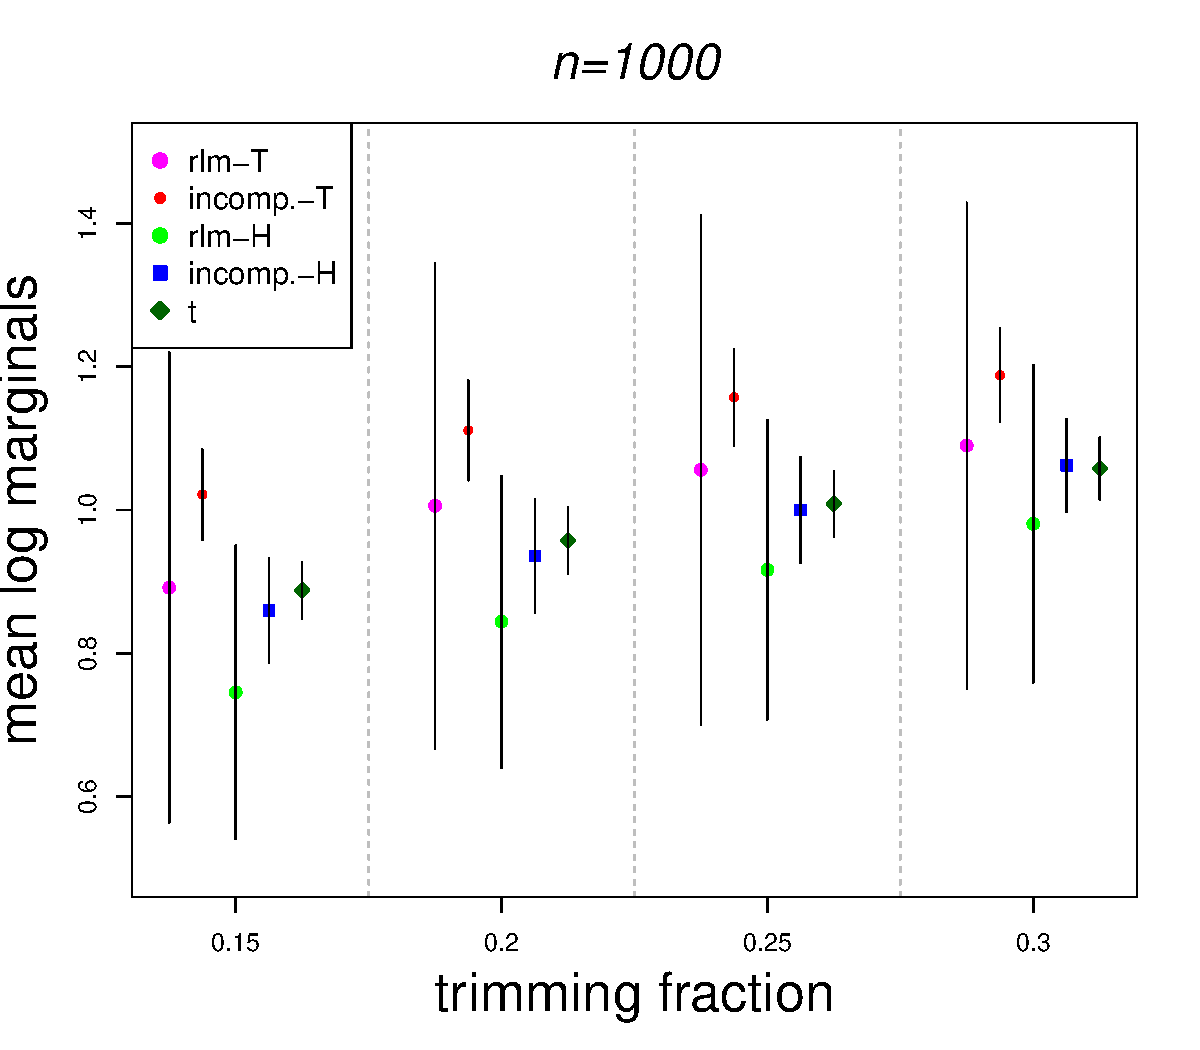
\includegraphics[width=2.75in,page=1]{hierlogMargType1AgenciesBaseModelt}}\quad
%%\subcaptionbox{}{\includegraphics[width=2.75in,page=2]{hierlogMargType1AgenciesBaseModelt}}
%\subcaptionbox{}{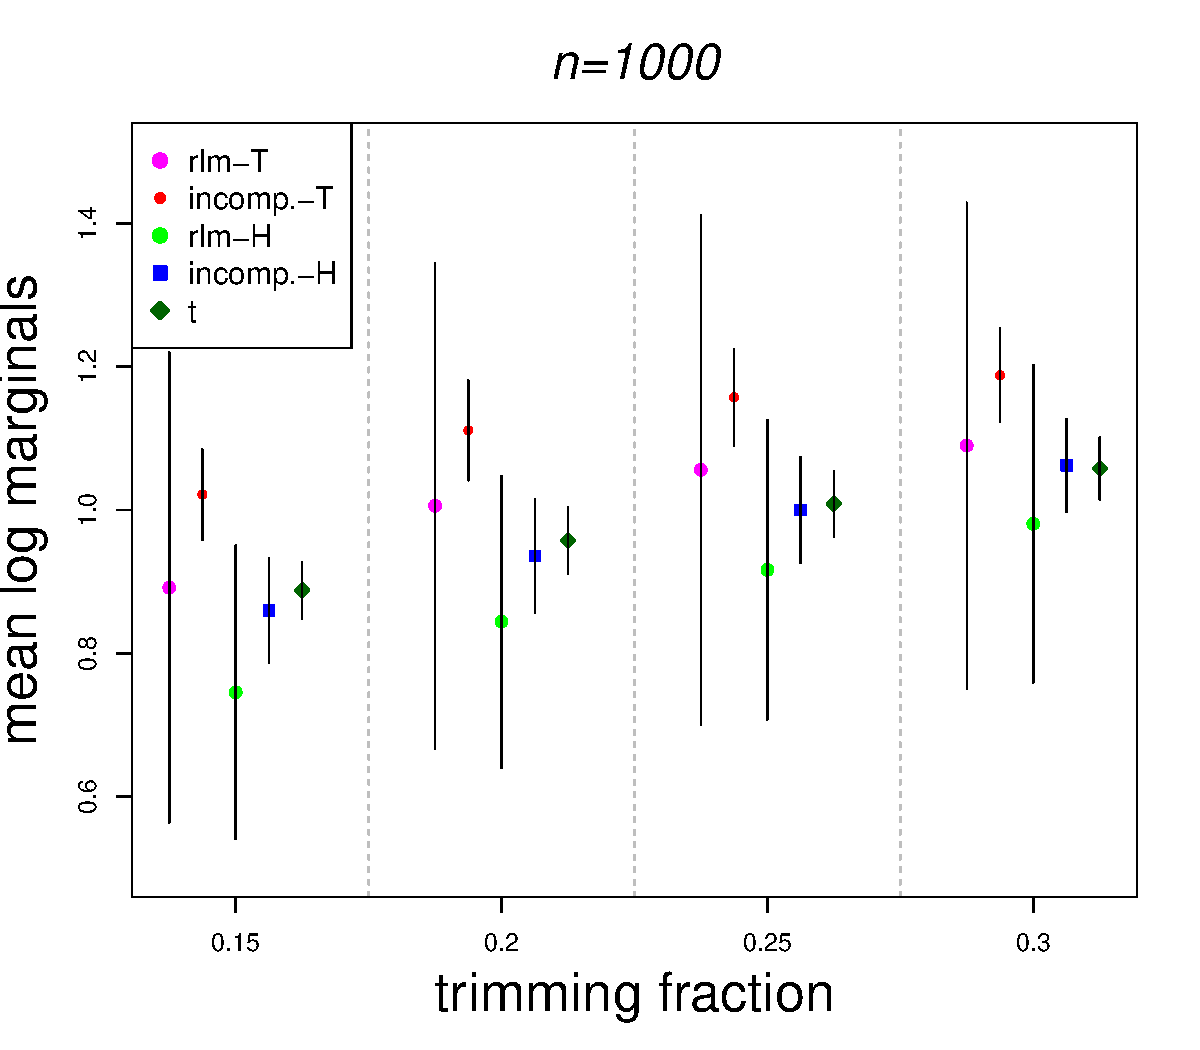
\includegraphics[width=4in,page=1]{hierlogMargType1AgenciesBaseModelt}}\quad
%\subcaptionbox{}{\includegraphics[width=4in,page=2]{hierlogMargType1AgenciesBaseModelt}}
%\caption{Model evaluation for `Type 1' agencies under the hierarchical model for $n=1000$ and $2000$. The $t$-model is used as the base method to compute TLM. Plotted are the mean TLM for each model against the trimming fraction across the $100$ cross-validation samples. Error bars correspond to one standard deviation of TLM above and below the mean. Models are labeled using the same notation as the previous figure. Only the relevant trimming fractions ($\alpha\geq .15$) are pictured.  
%}
%\label{fig:hierType1Marg}
%\end{sidewaysfigure}
%

%
%\subsection{Comparison of hierarchical and non-hierarchical fits}
%
%The performance of the methods for the hierarchical and non-hierarchical models can be contrasted through our cross validations studies.  We focus on Tukey's and Huber's conditioning statistic and concentrate our evaluation on the `Type 1' agencies. Table~\ref{tab:tlmTable} displays the mean TLM for each model and range of trimming fractions.  Our summary below focuses exclusively on realistic trimming fractions, $\alpha \geq 0.15$, and Tukey's conditioning statistic.  
%
%We first note that for the non-hierarchical model, there is little difference between mean TLM for $n=1000$ and $n=2000$, with 
%the numbers differing only in the third decimal place (see rows 1 and 3 of the table).  This is due to the posterior predictive distributions having stabilized.  The
%mean TLMs for the hierarchical model show a greater change with increases of about $0.05$ to $0.08$ as the training sample size changes
%from $1000$ to $2000$ (see rows 2 and 4 of the table).  For calibration, the mean TLM for a normal with mean $0.5$ and variance $1$ is approximately this size
%when trimming is done under a standard normal base model.  Thus, the increase in mean TLM is substantial.  
%We attribute the change for the hierarchical model to the 
%improvement in fits, particularly for states with fewer agencies.  
%
%Direct comparison of the hierarchical and non-hierarchical models shows that, for $n=1000$, the non-hierarchical model has uniformly 
%(for $\alpha$ of interest) better mean TLM (rows 1 and 2).  The differences are substantial, and the summaries primarily reflect greater stability of fits on a state-by-state basis under the non-hierarchical model.  To a lesser extent, they reflect variation in the evaluation criterion which stems from modest validation sample size, particularly with larger trimming fractions.  The trimmed cases are not proportionally distributed across states.  The pattern changes for $n=2000$ (rows 3 and 4), with the hierarchical model showing larger mean TLMs for trimming fractions $0.15$ and $0.20$.  The improvement reflects the ability of the hierarchical model to capture differences in regressions across the states which is realized when the training sample size is large enough.  We attribute the better performance of the non-hierarchical model for the largest trimming fractions to variation in the evaluation.  
%
%\begin{table}[!tbp]
%{\small
%\begin{center}
%\begin{tabular}{lllll}
%\hline\hline
%& \multicolumn{4}{c}{Trimming fraction ($\alpha$)}\\
%\multicolumn{1}{l}{}&\multicolumn{1}{c}{$0.15$}&\multicolumn{1}{c}{$0.2$}&\multicolumn{1}{c}{$0.25$}&\multicolumn{1}{c}{$0.3$}\tabularnewline
%\hline
%{\mdseries Tukey ($n=1000$)}&&&&\tabularnewline
%~~Non-Hier.&1.072 (0.014)&1.179 (0.022)&1.226 (0.029)&1.255 (0.033)\tabularnewline
%~~Hier.&1.021 (0.063)&1.110 (0.070)&1.157 (0.067)&1.187 (0.065)\tabularnewline
%\hline
%{\mdseries Tukey ($n=2000$) }&&&&\tabularnewline
%~~Non-Hier.&1.068 (0.029)&1.178 (0.007)&1.225 (0.011)&1.254 (0.014)\tabularnewline
%~~Hier.&1.094 (0.041)&1.189 (0.036)&1.221 (0.033)&1.242 (0.028)\tabularnewline
%\hline
%{\mdseries Huber  ($n=1000$)}&&&&\tabularnewline
%~~Non-Hier.&1.020 (0.020)&1.114 (0.035)&1.157 (0.041)&1.184 (0.045)\tabularnewline
%~~Hier.&0.861 (0.073)&0.937 (0.079)&1.001 (0.074)&1.063 (0.064)\tabularnewline
%\hline
%{\mdseries Huber ($n=2000$)}&&&&\tabularnewline
%~~Non-Hier.&1.015 (0.021)&1.112 (0.014)&1.154 (0.019)&1.181 (0.023)\tabularnewline
%~~Hier.&0.930 (0.041)&1.014 (0.043)&1.080 (0.035)&1.148 (0.027)\tabularnewline
%\hline
%\end{tabular}
%\end{center}
%\caption{Mean (standard deviation) of TLM for `Type 1' agencies for the Bayesian restricted likelihood non-hierarchical and hierarchical models for $n=1000$ and $2000$.} \label{tab:tlmTable}
%}
%\end{table}
%

\section{Discussion}
\label{Conclusions}

%In this work, we have presented an approach which begins to reconcile Bayesian methods with the practice of data analysis.
Many routine choices in an analysis react to the gap between reality and the
statistical model, where a bit of set-up work improves inferential
performance.  Often, these choices can be recast in the framework of
restricted likelihood presented here, lending them more formality and facilitating
development of theoretical results.  But a much greater benefit of our
framework is that it leads us to blend classical estimation with
Bayesian methods.  Here, we use the likelihood from robust regression
estimators to move from prior distribution to posterior distribution.
Conditioning on the estimator, the update follows Bayes' Theorem
exactly.   Computation is driven by MCMC methods, requiring only a modest supplement to existing algorithms.  In another context, we might condition on the results of a set of estimating equations, designed to enforce lexical preferences for those features of the analysis considered most important, yet still producing inferences for secondary aspects of the problem. For example, the computational strategies we devised here allow us to apply the method to inference on quantiles of a regression model. In other settings, we envision conditioning on a mix of estimators and some of the observed data.  

The framework we propose allows us to retain many benefits of Bayesian methods:  it requires a full and complete model for the data; it lets us combine various sources of information both through the use of a prior distribution and through creation of a hierarchical model; it guarantees admissibility of our decision rules among the class based on the summary statistic $T(\by)$; and it naturally leads us to focus on predictive inference.   

This same framework retains many of the benefits of classical estimation.  Great ingenuity has been used to create a wide variety of estimators in this tradition, many of which are designed to handle specific flaws in the model.  The estimators are typically accompanied by asymptotic results on consistency and distribution.  Many of these results carry over to our blend of classical and Bayesian methods, although regularity conditions differ.  We expect our procedures to have strong large sample performance, especially in settings where
pooling of information is of value.  

This framework opens a number of questions, including a need to revisit such issues as model selection, model averaging for predictive performance, and the role of diagnostics.  Perhaps the biggest question is which summary statistic to choose.  For this, we recommend a choice based on the analyst's understanding of the problem, model, reality, deficiencies in the model,  inferences to be made, and the relative importance of various inferences.  \green{In our words, to provide desireable inference, we recommend use of robust and relevant summary statistics in conjunction with Bayesian models.}  


\section{Appendix}
\label{sec:appendix}
\subsection{Proofs}
\noindent

Proof of Theorem~\ref{Transformation}.  
\begin{proof} 
\begin{eqnarray}
 s(X,\by) & = & s\left(X,\frac{s(X,\by_{obs})}{s(X,\bz^*)}\bz^* + X\left(\bb(X,\by_{obs}) - \bb(X,\frac{s(X,\by_{obs})}{s(X,\bz^*)}\bz^*)\right)\right) \\
& = & \frac{s(X,\by_{obs})}{s(X,\bz^*)} s(X, \bz^*)= s(X,\by_{obs}) , \qquad \mbox{and} \\
 \bb(X,\by) & = & \bb\left(X,\frac{s(X,\by_{obs})}{s(X,\bz^*)}\bz^* + X\left(\bb(X,\by_{obs}) - \bb(X,\frac{s(X,\by_{obs})}{s(X,\bz^*)}\bz^*)\right)\right) \\
 & = & \bb(X,\frac{s(X,\by_{obs})}{s(X,\bz^*)}\bz^*) + \bb(X,\by_{obs}) - \bb(X,\frac{s(X,\by_{obs})}{s(X,\bz^*)}\bz^*) \\ &=& \bb(X,\by_{obs})
\end{eqnarray}
\end{proof}

\noindent
Proof of Lemma~\ref{gradSTheoremReg}.
\begin{proof}
We first show that $\nabla s(X,\by)\in \mc{C}^\perp(X)$. Recall that
$H=I-Q$. By the regression invariance property \ref{regIn} of $s$, we have
\label{perpGradReg}
\begin{equation}
\label{eq:lem3.2}
\begin{aligned}
s(X,\by)=s(X, Q\by+H\by)=s(X, Q\by).
\end{aligned}
\end{equation}
Thus, by the chain rule $\nabla s(X,\by)=Q\nabla s(X,Q\by)=Q\nabla s(X, \bz)$. Hence $X^\top \nabla s(X,\by)=0$ as desired.
From equation~\eqref{eq:lem3.2}, all vectors $\bz'\in \Pi(\mathcal{A})$ satisfy $s(X,\bz')=
s(X,\by)=s(X,\by_{obs})$, and so all directional derivatives of $s$ along each tangent $\bv$ to
  $\Pi(\mathcal{A})$ in $\mc C^\perp(X)$ at $\bz$ are equal to 0 (i.e., $\nabla s(X,\bz) \cdot \bv=0$).  Thus $\nabla s(X,\bz)$ is orthogonal to  $\Pi(\mathcal{A})$ at $\bz$.  
Since $\Pi(\mathcal{A})$ has dimension $n-p-1$, $\nabla s(X,\bz)$ gives the unique (up to scaling and reversing direction) normal in the $n-p$ dimensional $\mc C^\perp(X)$.  
\end{proof}

\noindent
Proof of Lemma~\ref{lem:basis}

\begin{proof}
Without loss of generality, assume the columns of $X$ form an
orthonormal basis for $\mc C (X)$ and likewise the columns of $W$ form
and orthonormal basis for $\mc C^\perp(X)$. With earlier notation,
$H=XX^{\top}$ and $Q=WW^{\top}$. The set $\mc A$ is defined by the
$p+1$ equations  $s(X,\by)=s(X,\by_{obs})$, 
$b_1(X,\by)=b_1(X,\by_{obs}),\dots,  b_p(X,\by)=b_p(X,\by_{obs})$. Consequently, the gradients are orthogonal to $\mc A$. Let  $\nabla\bb(X,\by)$ denote the $n\times p$ matrix with columns $\nabla b_1(X,\by),\dots, \nabla b_p(X,\by)$. We seek to show the $n \times (p+1)$ matrix $[\nabla\boldsymbol\bb(X,\by),\nabla s(X,\by)]$ has rank $p+1$. Using property \ref{regEq}, we have that 
\[
\bb(X, \by)=\bb(X,Q\by+H\by)=\bb(X, Q\by)+X^\top \by
\] 
Then $\nabla \bb(X,\by)=Q\nabla\boldsymbol\bb(X, Q\by)+ X$ and 
\begin{eqnarray}
\label{BigMatrix}
[XX^\top, WW^\top]^\top[\nabla\boldsymbol\bb(X,\by),\nabla s(X,\by)]=
 \left( \begin{array}{cc}
X & \mathbf{0} \\
WW^\top\nabla b(X,\by)  &\nabla s(X,\by)  \\ \end{array} \right)
\end{eqnarray}
The last column comes from Lemma \ref{gradSTheoremReg}. The matrix $[XX^\top, WW^\top]^\top$ is of full
column rank (rank $n$), and so the rank of $[\nabla\boldsymbol\bb(X,\by),\nabla s(X,\by)]$ is the same as the rank
of the matrix on the right hand side of (\ref{BigMatrix}).  This last
matrix has rank $p+1$ since $\nabla s(X,\by) \ne \bzero$ by \ref{scaleEq2Reg}, and so does 
$[\nabla b(X,\by),\nabla s(X,\by)]$.
\end{proof}

\noindent
Proof of Lemma~\ref{lem:fullrank}

\begin{proof}
$P$ is the projection of the columns of $A$ onto $\mc
C^{\perp}(X)$. For this to result in a loss of rank, a subspace of
$\mc T_{y}(\mc A)$ must belong to $\mc C(X)$.  Following property
\ref{regEq}, for an arbitrary vector $X \bv \in \mc C(X)$, $\bb(X,\by
+ X \bv) = \bb(X,\by) + \bv$.  From the property, we can show that the directional derivative
  of $\bb$ along $X \bv$ with $\bv \ne \bzero$ is $\bv$, which is a
  nonzero vector. Hence $X\bv \notin \mc T_{y}(\mc A)$.  
\end{proof}

\noindent
Proof of Corollary~\ref{theorem:sings}

\begin{proof}
The corollary relies on a lemma and theorem from \cite{miao1992} which we restate 
slightly for brevity of presentation.  The principal angles between subspaces pluck off a
set of angles between subspaces, from smallest to largest.  The number of such angles 
is the minimum of the dimensions of the two subspaces.  Miao and Ben-Israel's first result
(their Lemma 1) connects these principal angles to a set of singular values, and hence to 
volumes.   
\begin{lemma}{(Miao, Ben-Israel)}
\label{MBI:lemma}
Let the columns of $Q_L\in \mathbb{R}^{n\times l}$ and $Q_M\in
\mathbb{R}^{n\times m}$ form orthonormal bases for linear subspaces
$L$ and $M$ respectively, with $l \leq m$. Let $\sigma_1\geq\cdots\geq
\sigma_l\geq0$ be the singular values of $Q_M^\top Q_L$. Then $\cos
\theta_i=\sigma_i, i=1,\dots,l$ where $0\leq\theta_1\leq\theta_2\leq
\cdots \leq\theta_l\leq\frac{\pi}{2}$ are the principal angles between $L$ and $M$.  
\end{lemma}

Miao and Ben-Israel's second result (their Theorem 3) makes a match between the principal
angles between a pair of subspaces and the principal angles between their orthogonal complements.  
\begin{theorem}{(Miao, Ben-Israel)}
\label{MBI:thm}
The nonzero principal angles between subspace $L$ and $M$ are equal to the 
nonzero principal angles between $L^\perp$ and $M^\perp$.
\end{theorem}

To establish the corollary, we appeal to Lemma~\ref{MBI:lemma} and Theorem~\ref{MBI:thm}.  Translating Miao and Ben Israel's
notation, we have $M=\mc C^\perp (X)$, $Q_M=W$, $L=\mc
T_{\boldsymbol{y}}(\mc{A})$, and $Q_L= A$. By Theorem~\ref{MBI:thm}, the
nonzero principal angles between $\mc{T}_{\boldsymbol{y}}(\mc{A})$ and
$\mc C^\perp(X)$ are the same as the nonzero principal angles between
$\mathcal{T}_{\boldsymbol{y}}^\perp(\mathcal{A})$ and $\mc C(X)$. By
\ref{MBI:lemma}, the non-unit singular values of $W^\top A$ are the
same as the non-unit singular values of $U^\top B$.  
\end{proof}

\subsection{Setting the hierarchical prior values}
In setting the priors we use the same previous data set used to set the priors for the non-hierarchical model (Section \ref{regModelNW}) and several heuristic arguments. While the analyses in Section \ref{hierRegNW} set the hyper-parameters using what is described here, the results were not sensitive to these choices.  This section describes the heuristics used in setting these prior parameters and is given for completeness. Using the previous data set we fit separate (robust) regressions to each state and a  regression to the \green{\sout{entire} entirety of the} data at once. Let the estimates for the fits to each state be $\hat{\beta_{1}}, \dots, \hat \beta_{J}, \hat \sigma_{1}, \dots, \hat \sigma_{J}$ and the estimates from the single regression be $\hat \beta$ and $\hat \sigma$. These are classical robust estimates using Tukey's regression and Huber's scale. Let $n_{j}$ denote the number of observations in the $j^{th}$ state and set $n=\sum n_{j}$. 

First, consider $v_{1}$ and $v_{2}$ in the prior $b\sim\text{beta}(v_{1},v_{2})$.  In the hierarchical model \eqref{eq:hierModel}, $b=0$ implies all the $\bbeta_{j}'s$ are equal (no variation between states) and $b=1$ implies the $\bbeta_{j}'s$ vary about $\mu_{0}$ according to $\Sigma_{0}=n\cdot \mbox{var}(\hat\beta)$ (see Section \ref{regModelNW}). We seek a prior measure for what we think $b$ should be. In other words, how much prior uncertainty should we allow in $\bbeta$ as opposed to the uncertainty amongst the $\bbeta_{j}'s$? Using the prior fit, a measure for  uncertainty for $\bbeta$ is $\Sigma_{\hat\beta}=\mbox{var}(\hat\beta)$, the estimate of the covariance from the single regression. For the $\bbeta_{j}'s$, take $\delta_{j}=\hat\beta_{j}-\hat\beta$ and set the prior uncertainty to $\Sigma_{\delta}=n^{-1}\sum n_{j}\delta_{j}\delta_{j}^{\top}$. Consider the value $g= \left(|\Sigma_{\delta}|/|\Sigma_{\hat\beta}|\right)^{1/p}$. Heuristically, $g$ is measure of the amount of uncertainty between the $\bbeta_{j}'s$ to the amount of uncertainty in $\bbeta$. Now in the prior, we heuristically set the uncertainty in the $\bbeta_{j}'s$ ($b\Sigma_{0}$) to be approximately equal to $g\cdot\mbox{var}(\hat\beta)$. That is, $b\Sigma_{0}\approx g\cdot\mbox{var}(\hat\beta)= \frac{g}{n} \Sigma_{0}$, suggesting $b\approx  \frac{g}{n}$.  Hence we set $E[b]=\frac{g}{n}$. The precision, $v_{1}+v_{2}$, is set to be relatively high at $20$, completing the specification for the prior on $b$. 

In setting the parameters for the beta prior on $\mu_{\rho}$ and gamma prior on  $\psi_\rho$ we first take $\hat z_{j}= \Phi^{-1} (H(\hat\sigma_{j}^{2}))$. As in the prior we assume $(\hat z_1,\dots,\hat z_J)\sim N_J(\mathbf{0}, \Sigma_\rho)$ with
$\Sigma_\rho=(1-\rho)I+\rho \mb{1}\mb{1}^{\top}$ and find the MLE, $\hat\rho_{mle}$, and observed inverse Fisher information, $I^{-1}(\rho_{mle})$. The mean of the beta prior on $\mu_{\rho}$ is set to $\hat\rho_{mle}$. Its variance is inflated somewhat and set to $2I^{-1}(\hat\rho_{mle})$. Since $\text{var}(\rho|\mu_{\rho}, \psi_{\rho})=\mu_{\rho} (1-\mu_{p})/(\psi_{\rho}+1)$ we replace $\mu_{\rho}$ with $\hat\rho_{mle}$, $\text{var}(\rho|\mu_{\rho}, \psi_{\rho})$ with $2I^{-1}(\hat\rho_{mle})$, and set the mean of the gamma prior on $\psi_{\rho}$ equal to $\hat\rho_{mle} (1-\hat\rho_{mle})/(2I^{-1}(\hat\rho_{mle}))-1$. Finally, we  set the rate parameter to 1 implying the variance of the gamma prior is equal to its the mean.
%The variance was set to twice the inverse Fisher information evaluated at $\hat\rho_{mle}$

%
%Plugging the estimates of $z_j$ into the multivariate normal, the mean of $\mu_\rho$ is set to the MLE of $\rho$ and the variance is set to the observed inverse Fisher information matrix, inflated by a factor of $2$ to weaken the prior for this parameter.  We use the same MLE and inflated information matrix to set the mean for $\psi_{\rho}$. Its variance is chosen to cover a range of plausible values. A range of other values for the fixed hyper-parameters was also studied.  The differences in results were negligible. 


\bibliographystyle{ba}
\bibliography{refPaper1}

\end{document}



